\documentclass[hidelinks,12pt]{report}
\usepackage{graphicx}
\graphicspath{ {images/} }

\usepackage[utf8]{inputenc}
\usepackage{adjustbox}

\usepackage{array}
\newcolumntype{P}[1]{>{\centering\arraybackslash}p{#1}}
\newcolumntype{M}[1]{>{\centering\arraybackslash}m{#1}}



\usepackage{float}

\usepackage{amsmath}
\usepackage{amsfonts}
\usepackage{amssymb}

\usepackage{listings}
\lstset{
    language=R,
    basicstyle=\ttfamily
}

\lstset{frame=tb,
  language=R,
  breaklines=true,
  showstringspaces=false
}



\usepackage{subcaption}


\usepackage{setspace}% http://ctan.org/pkg/setspace
% Already loaded by the apa6 documentclass...
\usepackage{etoolbox}% http://ctan.org/pkg/etoolbox
\AtBeginEnvironment{tabular}{\singlespacing}% Single spacing in tabular environment



\usepackage[left=2cm,right=2cm,top=2cm,bottom=2cm]{geometry}
\usepackage[authoryear,round]{natbib}

\usepackage[singlelinecheck=false]{caption}

\usepackage[pagestyles]{titlesec}

\setcounter{secnumdepth}{4}


\makeatletter
\newcommand*{\centerfloat}{%
  \parindent \z@
  \leftskip \z@ \@plus 1fil \@minus \textwidth
  \rightskip\leftskip
  \parfillskip \z@skip}
\makeatother

\titleformat{\chapter}[display]{\normalfont\bfseries}{}{0pt}{\Huge}
\newpagestyle{mystyle}
{\sethead[\thepage][][\chaptertitle]{}{}{\thepage}}
\pagestyle{mystyle}

\usepackage{setspace}
\doublespacing

\usepackage{textcomp}

\usepackage{hyperref}

\vspace{-\baselineskip}
\usepackage[english]{babel}

\begin{document}

\frontmatter
\pagenumbering{roman}


\begin{titlepage}
    \begin{center}
        \vspace*{1cm}
        
        \textbf{\Large Economic Implications of a Changing Yield Weather Relationship}
        
        
        \vspace{1.0cm}
        \singlespacing{\textbf{By}\\
        \textbf{Regan Arntz-Gray}
        }
         
      
        \vspace{2cm}
        \singlespacing{
        A Thesis \\
        presented to\\
        The University of Guelph\\
       \vspace{2cm}
        In partial fulfillment of requirements\\
        for the degree of\\
        Master's of Science\\
        in\\
        Food, Agriculture, and Resource Economics}
        
        \vspace{4cm}
       
       Guelph, Ontario, Canada\\
        \textcopyright \hspace{.1cm} \textbf{Regan Arntz-Gray, December, 2016}\\
        
        
    \end{center}
\end{titlepage}

\thispagestyle{empty}
\begin{center}
\Large
\textbf{\uppercase{Abstract}}
\end{center}
\medskip
\begin{center}
\large
\singlespacing
\uppercase{Economic Implications of a Changing Yield Weather Relationship }
\end{center}
\bigskip
\noindent
\textbf{Regan Arntz-Gray}
\hfill
\textbf{Advisor:\hspace{23mm}} \\
University of Guelph, 2017
\hfill
Professor Alan P. Ker
\bigskip
\\
\\
Average corn yield in Iowa and Ontario has significantly increased, potentially suggesting a corresponding increase in input demand. This implies that the yield-weather relationship may have changed over time. Yield modelling is used to test this hypothesis, and the results suggest that the yield-precipitation relationship is dynamic. To estimate the impact of neglecting the dynamic relationship, both a static and dynamic model were used to forecast yields given simulated weather from the current climate, as well as from a potential future climate. The yield forecasts were then used to estimate and compare the resulting actuarially fair premium rates. The results showed that using the static model led to biased premium rate estimates. Expected yield was calculated under both current and future climate. The mean expected yield was higher given climate change in Ontario but lower in Iowa. In both Iowa and Ontario, the variance of expected yield was higher under climate change.

\pagebreak





\thispagestyle{plain}
\addtocounter{page}{1}
\begin{center}
\Large
\textbf{\uppercase{Acknowledgements}}
\end{center}

The completion of this thesis project would not have been possible without the support of several individuals. First, I would like to thank my advisor Alan Ker. Despite my lack of economics background, Alan encouraged me to apply for the FARE program. His encouragement led to the completion of my masters, and enabled me to gain invaluable experience and skills. Alan's high academic standards and critical input elevated the quality and depth of this project. His renown as a researcher is well deserved. I would also like to thank my thesis committee member Bill Deen for his insight into the agronomic relationships underlying some of the questions addressed in this project, and the potential implications of our results. His knowledge in this area was crucial to the development of the empirical methods, and models used.

The academic culture in the FARE program has created an environment which is friendly and comfortable, as well as challenging for it's graduate students. This environment is maintained through the actions of everyone involved in the department. It has been a great place to learn, work, and make connections. In particular I would like to thank my fellow cohort of graduate students. The warmth and support provided has constantly exceeded expectation.

Finally, I would like to thank my family for your continual support and encouragement.  I attribute my academic curiosity in large part to my father, Jules, who started summarizing and explaining Scientific American articles to me when I was four.  To my mother, Janna, thank you for always being there for emotional support and for helping me to maintain perspective. You have both encouraged me to pursue my interests, and to always questions things. The environment you provided for me has made this easy to do, and your support is very much appreciated.


\tableofcontents



\pagebreak
\listoffigures
\pagebreak
\listoftables

 
\mainmatter

\chapter{Article}
\pagenumbering{arabic}
\input{chapters/Article}

\chapter{Introduction}
 \pagenumbering{arabic}

\section{Background and Motivation}

Agricultural production depends on several factors, of which only some are within a producer's control. While farm management choices are important to the success of crops, weather is a significant and uncontrollable determinant of crop yields. Farm incomes depend on yield which is inherently uncertain due to its reliance on weather. Farm incomes also depend on prices at the time of harvest, which further contributes to income uncertainty. The level of uncertainty faced by producers creates a market for income risk-reducing mechanisms such as crop insurance. Crop insurance programs are heavily subsidized in both the United States and Canada \citep{rosenzweig2002increased}. This effectively transfers a large portion of producer income risk to the public. In 2014 the total amount spent on risk management programs such as crop insurance by the public was nearly \$1.4 billion in Canada, while in the United States \$6.2 billion was spent on premium subsidies \citep{kerRMP2016}. Subsidized crop insurance programs comply with trade deals, and are therefore a popular method of transferring income to agricultural producers. These programs are subsidized to encourage producer participation in order to avoid the need for short-term disaster assistance programs \citep{coble2013we}. Historically, significant premium subsidies have had to be in place for participation to significantly increase \citep{goodwin2013harm}. 

Agricultural technology over the past 60 years has focused on increasing mean yields, as opposed to decreasing production risk. Corn yields in Iowa and Ontario increased more than three-fold over that time period \citep{CANy,NASSy}. As mentioned above, producers generally do not bear all of their income risk, due to the subsidization of crop insurance programs. This alters the rational production decision set, as farmers are less sensitive to the negative impacts of highly variable crop varieties. This could lead to producer demand for varieties with high mean yields, even if these high yields are attained at the expense of increased variability. Additionally, the change in the yield distribution in Ontario was found to be empirically consistent with the use of subsidized crop insurance as a substitute for other income risk reducing mechanisms \citep{kerRMP2016}. 

The large increase in mean yield since the 1950's was driven by several factors: increased attention to farm management practices such as time of planting, a large increase in nitrogen application from the 1950's to the 1980's, and a steady increase in plants per acre until present \citep{duvick2005contribution}. This increase in yield, and in particular in plants per acre, suggests an increase in demand for inputs per acre. Given the dependence on weather, not all agricultural inputs are in the control of producers. In particular, water is largely out of producer control as almost all corn acres are rain fed in both Iowa and Ontario. The large changes in plants and yield per acre suggest that the relationship between precipitation and yield may have changed over time. 

In addition to these changes, agricultural systems also face the impending effects of climate change. Climate change is expected to lead to more extreme heat events as well as more extreme precipitation events, both of which have the potential to be detrimental to corn yields \citep{rosenzweig2002increased,southworth2000consequences}. Many factors can impact the way in which crop yields will respond to climate change, such as the current temperature and precipitation distribution, and the type and quality of the soil. Top soil depth has been found to correlate with soil water capacity. This implies that regions with deeper top soils will likely be less sensitive to to drought conditions, as the precipitation received can be used more effectively. Deep top soils could therefore reduce the negative impact of extreme precipitation events \cite{lee2015topsoil}. Finally, increasing world population will likely lead to a corresponding rise in global demand for field crops. This increase in demand, coupled with climate change effects could threaten global food security \citep{edgerton2009increasing}. Given these considerations, it is important to consider the fragility and productivity of our food systems \citep{williams2016soil}.


\section{Economic Problem}

 The number of plants per acre, as well as average yields, have increased throughout the study period \citep{duvick2005contribution}. The increase in yield and plant populations per acre implies a potential increase in the level of inputs per acre needed to produce a relatively high yield. Given that most corn fields are rain fed in North America, the water input is essentially fully dependent on weather conditions. If the amount of water required per acre has increased, it is possible that the relationship between precipitation and yield may have changed over time. The magnitude of this change will likely depend to some degree on conditions affecting water uptake levels such as soil quality and depth. A change in the relationship between yield and precipitation could have implications regarding mean yields and the degree of yield variability. Yield variability is inherent in agriculture due to the reliance on weather which is, by nature, unpredictable. As producers rely on yields for their income, yield variability leads to income variability and therefore risk for producers. 

In addition to the possibility that the yield-weather relationship is changing, the distributions of key weather variables affecting corn yields are likely to be modified as a result of climate change. Since crop yields are dependent on weather, changes in weather patterns will also influence yield and income variability. The negative impacts of income variation, to which producers are subject, can be partially mitigated by participation in crop insurance programs \citep{rosenzweig2002increased}. Producers are faced with decisions regarding their crop insurance plans including what aspects of the farm to insure, and the level of coverage they would like. Under some plans the producer can also choose a fixed or floating claim price; a fixed claim price is determined based on price expectations at the start of the season, while a floating claim price is determined based on actual market conditions after harvest \citep{Agri2014, NCIS}. These decisions must be made based partially on the producer's expectation of yields and yield variability. The economic problem which motivates this research is how the changes in agricultural technology, coupled with potential climate change effects, will impact corn production, producer livelihoods, and the efficacy of crop insurance programs, through their effect on the yield weather dynamic.

The impact of weather, in particular precipitation level, on corn yields and how these impacts have changed over time will be investigated. The potential yield response to predicted climate impacts will then be considered based on the results of this investigation. The solution to this problem is important to producers and crop insurance providers as well as tax payers, as it will allow for more accurate short term and long term predictions of yields, given accurate weather and climate forecasts. The improved ability to predict yields may help producers better cope with the levels of weather and climate related risk associated with crop farming. Information regarding yield forecasts under climate change could aid producers in making decisions which allow them to adapt their production systems in their best interest. Since crop insurance premia are set, in part, based on estimates of crop yield distributions, improved yield forecasts may lead to more accurate estimates of expected losses. Crop insurance providers need to maintain financial soundness over time, meaning that the total indemnities paid must equal the total value of premiums and subsidies collected. Accurate estimates of  yield distributions could aid in the ability of insurers to set premiums in such a way, and to insure that the reserve fund balance is kept at an appropriate level. Since crop insurance programs are subsidized to some degree by government, their efficient operation is desirable for the general public as well. Finally, a basic understanding of how food systems are affected by weather could assist in large scale and long term planning. This understanding could inform the best way to adapt these systems to the changing underlying conditions which may arise due to the intersection of climate change, and changes in agricultural technology.

\section{Economic Research Problem}

The economic research problem is how to construct a weather dependent corn yield model which changes through time. This model can then be used, along with simulated weather data from possible future climate scenarios, to estimate how yield may be affected under climate change, and how this will impact crop insurance rates. Solving this problem will allow for the consideration of possible consequences of the intersection of a changing yield-weather dynamic and climate change. The results of this study could be used to inform adaptation strategies at the individual as well as national levels. 

The yield-weather response function will be determined using historical data. The precipitation-yield relationship will be modelled such that the effect of precipitation on yield is dynamic through time. This is done in order to allow for, and subsequently test, the possibility that changes in agricultural technology may have modified the yield weather model. This research will aid in the understanding of the impact of weather on corn yields. This understanding, in conjunction with estimates of current and future weather distributions, could be used to inform the levels of crop insurance premia. Since crop insurance in Ontario and Iowa is subsidized by government to a large extent this research is also relevant to tax payers. The ability to forecast yield under predicted climate change scenarios will allow for the investigation of the effect of climate change on the mean and variance of expected corn yields.  Estimating the nature of climate change effects on crop yields will allow for planning and development of appropriate adaptation strategies. 

This research falls into the class of problems which deal with producer risk and uncertainty in the insurance market. The potential changes in the yield climate relationship could lead to changes in the estimated level of production risk, while the dependence on weather implies continued uncertainty. Although the proposed research focuses only on corn in Ontario and Iowa, this research question could be asked of other crops grown in different locations, and approached using similar methods. While there will likely be differences in the effects of weather on various types of crops grown in a range of climatic conditions, the overall framework of determining relationships between various weather variables and yield over time and using those results to improve information in the crop insurance market could be applied elsewhere. 

\section{Purpose and Objectives}

The purpose of this study is to determine whether or not there is evidence to suggest that the relationship between corn yield and precipitation has changed over time. The potential consequences of these results on the ability to accurately predict yield distributions will be considered in terms of its effect on the estimation of the actuarially fair level of crop insurance premia. Finally, the consequences of climate change given the findings regarding the yield weather relationship will be investigated.

The objectives of this research are:

\begin{enumerate}
 \item To review the literature in order to determine the most appropriate explanatory variables to include in a crop yield model.
  \item To develop a conceptual framework of corn yield in relation to weather variables which can change through time, and use this framework to develop an empirical model.
  \item To estimate this empirical model, and determine whether there is evidence for a changing yield precipitation relationship over time.
  \item To consider the effect that the possibly dynamic yield precipitation relationship could have on the estimation of yield distributions and the actuarially fair premia level.
  \item To consider the possible implications of these results under potential climatic changes.

\end{enumerate}
 
The yield-weather relationship will be modelled using historical data, such that the precipitation effect can change through time. The effect of particular weather variables on yield, such as total precipitation at key growth stages, will be estimated. Given simulated weather realizations from both the current climate and a potential future climate, this model will be used to forecast yields so that the possible effects of climate change on corn yield can be considered. The effect of allowing for the potentially dynamic yield precipitation relationship on the resultant yield distribution estimates will be discussed in terms of its effect on the calculation of the actuarially fair level of crop insurance premia. 



\chapter{Literature Review}
\section{Trends in Corn Yield in North America}

Average yields in both Canada and the U.S have been increasing over the entire study period \citep{CANy, NASSy}. Figures 2.1 and 2.2 show the average  corn yields, in both Iowa and Ontario, for the years considered in this study.

\begin{figure}[!hb]
  \centering
  \begin{minipage}[b]{0.45\textwidth}
    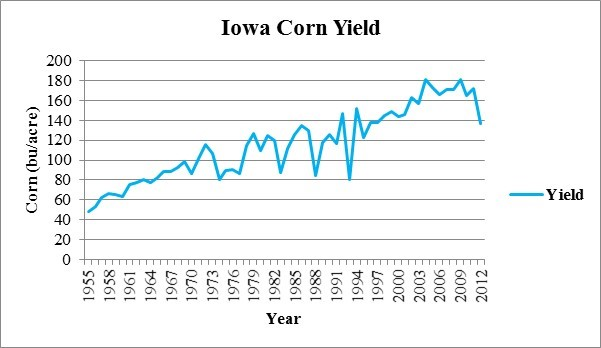
\includegraphics[width=\textwidth]{CornYieldIowa.jpg}
    \caption{Corn Yield (bu per acre) Iowa: 1955-2012 (NASS)}
  \end{minipage}
  \hfill
  \begin{minipage}[b]{0.45\textwidth}
    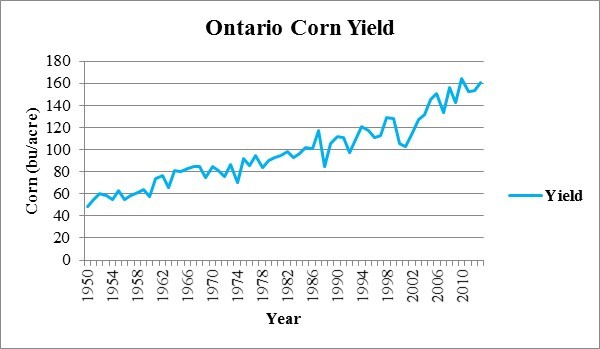
\includegraphics[width=\textwidth]{CornYieldOntario.jpg}
    \caption{Corn Yield (bu per acre) Ontario: 1950-2013 \citep{CANy}}
  \end{minipage}
\end{figure}

These figures show that average yield, in both Ontario and Iowa, has risen substantially over this period. The increase in yield has largely been the result of improved hybrids, and other agricultural technologies \citep{edgerton2009increasing}. In particular, the number of plants per acre has increased at a rate of approximately 400 plants per acre per year over the past 50 years in the central US cornbelt \citep{duvick2005contribution}. Each plant theoretically requires input levels to be within particular ranges and combinations in order to attain a high level of production. Thus, as the number of plants per acre increases, there is likely to be a change in the total level of inputs per acre required to attain relatively high yields. Changes can be made to  agricultural management practices in order to accommodate the needs of increased plants per acre, for example, the amount of fertilizer can be increased, or techniques to improve the water holding capacity can be undertaken. However, some of the inputs affecting corn yield are out of producer control, such as precipitation. Given that poor weather conditions can decimate yields while ideal conditions cannot increase yields beyond their biological potential, corn yield distributions are generally negatively skewed \citep{tolhurst2014technological}. According to \cite{tolhurst2014technological}, yield outcomes can be separated into `regular' and `poor' years in order to reflect this characteristic of yield distributions. The 2011 census of agriculture reports that less than 1\% of all farm acres in Ontario are irrigated \citep{CANirrigation, CANcensus}. In general, almost all corn in North America is grown without irrigation, and therefore water input levels depend almost solely on weather patterns. If a higher level of precipitation per acre is needed to attain high yields, this would increase the likelihood that precipitation will be a limiting factor in any given year.  This could result in an increase in the probability of a `poor' yield year, as precipitation would be a limiting factor more often. At the same time, precipitation levels which are too high can also be damaging. When too much precipitation occurs in a short period of time it can damage crops through flooding as well as by increasing the soil moisture which can heighten the risk of plant disease and infestation, delaying both planting and harvesting \cite{rosenzweig2002increased}. It would be expected that an increase in plants per acre would raise the maximum beneficial level of precipitation,  due to the presumably elevated demand for water. However, the heightened density of plants per acre could also result in higher levels of competition for soil nutrients which could be depleted by heavy rainfall. Therefore, the resulting effects of the interplay of changing agricultural technology, farm management practices, and weather is complex.

\section{Crop Insurance}

Agricultural producers face income uncertainty which can be decreased through participation in programs such as crop insurance. Given that this research is based on yield levels, the crop insurance programs  discussed are those which guarantee yield as opposed to  other measures of producer livelihood such as profit margins or whole farm income. Crop insurance for corn is government subsidized in both Iowa and Ontario in order to help producers access a low cost income risk mitigation tool. As discussed in the introduction, subsidization transfers  a portion of production risk to the public, and is done to increase participation in crop insurance programs. High risk production choices are therefore relatively more attractive to producers than they would be without subsidization, which suggests that production decisions could be distorted by these programs. In \cite{goodwin2013harm}, corn acreage at the county level was found to increase with mean subsidy rate in the US, supporting this claim \citep{goodwin2013harm}. \cite{kerRMP2016} demonstrated that the change in corn yield distributions in Ontario have shifted the upper end of the yield distribution up more quickly than the lower end \citep{kerRMP2016}. This observation is consistent with producers using crop insurance as a substitute for other risk reducing practices. The benefit to producers from subsidized crop insurance is significant, \cite{goodwin2013harm} estimate that in the US ``each dollar of premium paid by farmers tends to yield approximately \$1.90 in indemnity payments". As a result, producers may engage in rent seeking behaviour in order to increase subsidies, or at least prevent their decrease \citep{coble2013we, kerRMP2016}. 

The Production Insurance (PI) program in Ontario and the yield guarantee (YG) program in Iowa provide insurance on the total level of production. These programs pay out when realized yield is below some guaranteed level. In Ontario, the federal and provincial governments subsidize the PI program which is administered by Agricorp Ltd., a crown corporation \citep{li2014climate}. The YG program in Iowa is  subsidized by the federal government, and is administered by approved private insurance providers who operate within the rules and regulations set out by the Federal Crop Insurance Corporation (FCIC) \citep{NCIS}. More details about the crop insurance programs in each location are provided below.

\subsection{Ontario}

Agricorp administers crop insurance in Ontario. Agricorp's responsibilities include maintaining the stability of premium rates and the reserve fund balance, as well as the financial solvency of the program, in addition to acting as a safety net for producers. As mentioned above, the PI program is a yield guarantee program and is just one of the risk reducing programs which Agricorp manages. The level of yield which is guaranteed by the program depends on the historical yields of the individual producer, which are used to create a measure of average farm yield (AFY).  A coverage level is then chosen, and a payout is made if the actual yield falls below the coverage level times the AFY. For existing participants in the program the AFY is calculated using the average actual yield over the past ten years. New participants in the program are given a five year base average yield based on land quality and other factors. For each year they participate in the program, their actual yield goes into the calculation of AFY and one of the base average yield values is dropped until the AFY is an average of the participant's true historical yields \citep{Agri2014}.  The impact of overly high and low yield years on the AFY is mitigated by buffering these values. A yield value is subject to buffering if it is more than 1.3 times the current AFY, or less than 0.7 times the current AFY. If a given yield is over the upper boundary (1.3 times the AFY), it is adjusted to the level two-thirds of the way down between the actual yield realization and 1.3 times the AFY \citep{Agri2014}. For example, if the current AFY was 100 bu/acre, then a yield above 130 bu/acre would be subject to buffering. Say that the yield was 160, then this would be adjusted to 140 bu/acre which is 2/3 of the way down from 160 to 130. Similarly, a yield realization will be buffered up if it is below 0.7 times the current AFY before being added in to create the updated AFY calculation. This prevents any given year from having too large of an effect on the AFY.
 
Participants in the program are able to choose their coverage level (for corn the options are between 75 and 90 percent), as well as decide between a fixed and floating claim price \citep{Agri2014}. A claim price is the amount per bushel which will be paid to producers should their production fall short of their guaranteed production level, where the guaranteed production level is simply the coverage level times the AFY \citep{Agri2013}. A fixed claim price is calculated at the start of the season using projected prices, while a floating claim price is decided based on market prices at the time of harvest \citep{Agri2013}. Should the participant select the floating claim price they will be paid out at the final calculated price, regardless of whether this is higher or lower than the fixed price. The premia paid by the participants are based on the number of insured acres, a base premium rate, and surcharges or discounts based on the producer's previous claims to the program. The base premium rate depends on the previous year's rate and varies depending on the level of the reserve fund balance, the expected claim price, and past performance of the plan \citep{Agri2014}. Over time Agricorp is expected to balance the total insurance indemnities paid out with the total premia paid by participants and government contributions (ie. remain fiscally sound).  When weather and corresponding yield is predicted accurately, estimation of expected losses is closer to reality, and financial planning can be successfully undertaken. If climate change leads to increasingly variable weather patterns however this could become more difficult. Producers also make choices which depend on their expected yield and anticipated market conditions. When selecting their level of coverage and the type of premium they would like to pay, these expectations inform their decision making. These decisions are difficult to make without good weather predictions and an understanding of the relationship between weather and yield. Given that the federal and provincial governments bear a significant portion of the cost of crop insurance, the efficient operation of crop insurance programs is of interest to tax payers. This makes the changing yield-weather relationship something of concern not only to producers and insurance providers, but also to the general public.

\subsection{Iowa}


Crop insurance is provided through a private public partnership in the U.S., with producer paid premiums significantly subsidized through public funds \citep{NCIS}. The Federal Crop Insurance Program, which is administered under the United States Department of Agriculture (USDA) Risk Management Association (RMA), is responsible for overseeing the provision of crop insurance in the country.  The Federal Crop Insurance Committee (FCIC) sets program standards, premium rates, and subsidizes farmer premiums. In Ontario premium levels are set based on the levels in previous years, the level of the reserve fund, and, if the producer has been enrolled in the program for some time, discounts or surcharges based on past claims to the program. In Iowa premium levels depend on similar factors, however, unlike in Ontario, an individual producer's past claims to the program will not effect the rate they pay.  Premium rates are set by the Risk Management Association, and private insurers are required to provide insurance to any producer at the premium rate set by the RMA \citep{NCIS}. 

The provision of crop insurance is handled by approved private providers who share the risk with the public sector through a reinsurance agreement with the federal government. A measure of actual production history (APH), similar to the AFY measure in Ontario, is used to determine whether or not a payout will be made. Producers who are signing up for crop insurance for the first time have their APH calculated using historical yields which are proven using sales receipts, farm records or other methods \citep{ISU}. The APH is the average of a minimum of 4 years and a maximum of 10 years of records. If at least 4 years of records cannot be provided than a transition yield is provided to fill in each of the missing years. The transition yield is calculated based on the 10-year historical county level average yield \citep{ISU}. As with the buffering for the AFY in Ontario, mechanisms to prevent the APH from being modified by extreme yield values are in place. The proven yield, or APH, is not allowed to decline by more than 10\% in a given year. In addition, producers may request that any yield be replaced with a yield equal to 60\% of the transition yield, which allows them to reduce the impact of particularly low yield years \citep{ISU}. The price used in the event of a payout is forecast at the beginning of the season.  As in Ontario, the ability to accurately predict crop yields would aid insurance providers as well as producers in determining optimal premium rates and coverage levels respectively.


 

\section{Climate Determinants of Yield}

Weather is a significant determinant of crop growth, and the yield response to weather is complex. Weather determinants, such as heat and precipitation, do not have fixed effects on yields. This makes the determination of the effect of weather on yields difficult.  Evidence from the literature generally shows a nonlinear temperature effect. Higher temperatures are beneficial to corn growth but only until some maximum temperature is reached, at which point crops suffer from excess heat stress \citep{schlenker2009nonlinear}. Frost near the end of the corn season can also be responsible for significant yield decreases \citep{OMAFRA}, and temperatures below 2 degrees Celsius were found to be significant contributors to yield loss in \cite{tolhurst2015cold}. The effect of precipitation on yield is also non linear. Precipitation is a positive determinant of yields only when it comes at the right time and in the right amounts \citep{hansen1991farmer, tan2003impacts}. To further complicate the matter, the yield optimizing temperature has been found to shift depending on the amount of precipitation received and vice versa \citep{tan2003impacts, schlenker2009nonlinear}. Yield response to weather variables is also highly dependent on the crop growth stage, as different levels of inputs are required at different times (Dixon et al., 1994). In addition to the complications involved in determining the impact of weather on yields, the most appropriate measures of weather effects to use as explanatory variables for crop yield modelling is undecided. Different studies use a range of measurement techniques to capture similar weather effects relevant to crop yields. 


The weather dependent inputs which are generally considered to be of high importance in terms of their effect on corn yields are heat and water available to the crop. These effects can be measured in a myriad of ways. For example, heat effects can be measured by average temperature over the growing season, month, or growth stage \citep{ozkan2002impacts}, or by measures related to daily temperature such as growing degree days (GDD) \citep{swan1990corn}. Growing degree days are a measure of heat accumulation relative to a defined temperature range. Temperatures above 10 degrees Celsius allow for corn growth, and have an increasing positive impact on yield until they reach around 29 degrees Celsius \citep{neild1987growing}. This temperature range generally defines the space where temperature positively contributes to the measure of GDD. There are several methods for calculating growing degree days. \cite{snyder1985hand} proposes a method for calculating degree days based on daily minimum and maximum temperatures using a sin curve approximation. However, a simpler method which calculates GDD as the difference between the average of the maximum and minimum temperatures (up to an upper limit of around 29 degrees Celsius) and a base temperature is often used in the agronomic literature. This method is simpler to calculate and can be used to approximate the timing of corn growth stages \citep{neild1987growing}. Given that increases in temperature beyond around 29 degrees Celsius negatively and severely affect yields, measures to capture negative heat effects, such as extreme heat degree days (HDD), can also be included in yield models \citep{roberts2012agronomic}. Extreme heat degree days are also a cumulative temperature measure, however, as opposed to approximating the total amount of beneficial heat received by the plant it aims to approximate the amount of extreme heat.  The calculation of the HDD measure is therefore similar to that used for GDD, except that the HDD temperature range begins after the maximum GDD temperature range and has no upper limit.  Cold temperature stress can also affect corn yields especially in Northern areas, however measures of cold temperature are often not included in corn yield models. \cite{tolhurst2015cold} developed an analogous measure to GDD and HDD for cold and freezing temperature effects called cold degree days (CDD) and freezing degree days (FDD) respectively. These cold weather variables were included in the model used in \cite{tolhurst2015cold}, and CDD was found to have an economically and statistically significant effect on yield. This suggests that accounting for cold weather effects may be worthwhile in relatively northern contexts.

Levels of moisture available to the crop can also be measured in more than one way, for example the effect can be measured by total precipitation, average precipitation, maximum precipitation, or soil moisture \citep{dixon1994estimating}. The ability for soil to hold moisture has been found to increase with its depth by several studies \citep{lee2015topsoil, Guilpart}. Furthermore, the water holding capacity of soil has been found to be a positive yield determinant, and appears to lead to decreased yield variability by making plants less sensitive to low precipitation levels \cite{williams2016soil, lee2015topsoil}. Therefore, the effect of precipitation level on yield will likely be impacted by the soil type, quality, and depth. Given that these types of characteristics are often regional, this implies that the effect of climate change on yield could vary by location.   Vapor pressure deficit (VPD) is another variable used to measure moisture availability in crop yield models \citep{lobell2014greater,tolhurst2015cold}. VPD is a measure of the difference between the maximum amount of moisture which can be held in the air given the current temperature and the actual amount of moisture in the air. The ability of air to hold moisture is dependent on temperature, and therefore VPD measures a combination of heat and humidity effects. The variety of measures which can be used to track weather effects makes the choice of independent variables to include in a corn yield model non-trivial.

\section{Corn Yield Models with Weather Variables}

Studies of the impact of weather on yield use a variety of measures to represent the weather effects of interest.  In a study on weather and corn yield in Illinois from 1950 to 2010, \cite{roberts2012agronomic} found that  including VPD as an explanatory variable significantly increased model fit. This study used a linear functional form. VPD was found to have a positive effect on yields except in July and August. This exception is likely due to the extreme heat effects on corn yield which are most dangerous during this time and are reflected in high VPD. GDD and HDD were used to represent temperature effects in this model \citep{roberts2012agronomic}. It was found that the level of damage resulting from HDD was related to precipitation level, and that the minimum damage from HDD occurred when precipitation was near its average value  \citep{roberts2012agronomic}.  A statistical study in Turkey over the years 1975 to 1999 found that climate variables have a differential effect at each stage in the growing season \citep{ozkan2002impacts}. This study used a linear functional form and stepwise selection on wind, precipitation, temperature, and humidity variables calculated by growth stage to choose independent variables to be included in the model. They found that temperature, both at planting and harvesting time, was the most important indicator for corn yields \citep{ozkan2002impacts}. A second study in Illinois conducted at the crop reporting district level for years 1953 to 1987 estimated four linear models. Each model employed different combinations of soil moisture, precipitation, and temperature measured over growing season and month \citep{dixon1994estimating}. The results showed that conditioning weather on growth stage was superior to conditioning on month, and that omitting solar radiation as an explanatory variable reduced model fit. Between soil moisture and precipitation it was unclear which was the preferred variable to represent moisture available to the crop \citep{dixon1994estimating}.


In a county level US study over the period 1950 to 2005, \cite{schlenker2009nonlinear} found that temperature was a positive yield indicator until 29 degrees Celsius, in agreement with agronomic results. Additionally, this threshold level was found to be relatively stable over time. A linear functional form which allowed for spatially correlated errors was used to represent the yield weather relationship, with temperature effects measured using growing degree days. In order to consider the possibility that the effect of weather variables on yield changed based on precipitation levels, the model was estimated separately for each precipitation quartile so that the resulting coefficients could be compared. The results suggested that higher levels of precipitation could buffer the impacts of damage from extreme heat \citep{schlenker2009nonlinear}. The relationship between temperature effects and precipitation level was also noted in \citep{hansen1991farmer}. Another statistical study, using the same yield data as in \cite{schlenker2009nonlinear}, used linear and quadratic terms of monthly mean growing season temperature to measure heat effects \citep{urban2012projected}. They found that with this representation of temperature effects, adding in an additional variable for extreme heat days did little to improve the model given that high monthly temperature is well correlated with high numbers of extreme heat days \citep{urban2012projected}. The quadratic term was therefore able to represent the negative effect from extreme heat.

\cite{williams2016soil} studied weather effects on corn yield in Minnesota, Pennsylvania, Illinois, and Michigan using county level yield, soil characteristics, and weather data from 2000-2014. Higher precipitation levels were found to increase stability, while extreme heat and low precipitation decreased both stability and mean corn yield.

The level of yield volatility was found to be strongly affected by the soil water holding capacity in all four states, suggesting that management factors which affect this capacity could protect yield from extreme weather conditions \citep{williams2016soil}. The potentially negative yield effects from climate change demonstrate the importance of water supply to the plant \citep{williams2016soil}. Agricultural management practices can increase the ability of soil to hold water, and could therefore increase in importance as the effects of climate change begin to be felt \citep{ williams2016soil}. This also implies that the soil type and quality in a region could lead to differing effects under climate change. Loss of topsoil depth due to erosion has become an issue in Iowa \citep{IowaSWCS}. Deep topsoil generally has improved water holding capacity and nutrient retention and is therefore beneficial for crop yields, implying that erosion may have negative yield impacts \citep{lee2015topsoil}. \cite{lee2015topsoil} studied the effect of soil erosion on corn yields in the rain fed Iowa region using data from 2007 to 2012 collected from 7 farm sites with different soil types.	\cite{lee2015topsoil} considered relationships between soil depth, soil organic carbon content, and yield. The results demonstrated that increased topsoil depth and soil organic carbon content had a positive yield effect. High precipitation levels decreased the difference in yield based on top soil depth, and thereby increased stability levels.


\cite{tolhurst2015cold} conducted a study using county level de-trended yield data in Ontario. As mentioned above, cold weather effects are not generally considered in corn yield models. However, \cite{tolhurst2015cold} created analogous measures to GDD and HDD for cold weather effects, called cold and freezing degree days (CDD and FDD respectively), to include as explanatory temperature variables in addition to GDD and HDD. Moisture supply was accounted for using three different explanatory variables in the corn yield model. These were: accumulated monthly precipitation, a flood variable which tracks the number of days which had very high levels of precipitation (roughly corresponding to levels at or above the 99th percentile), and a variable called moisture supply-demand (MSD) which is calculated based on precipitation and VPD as used in \cite{urban2015impacts}. This study found that CDD was a statistically significant contributor to yield decreases. Precipitation was found to be a negative yield determinant at the start and end of the season (April and September) and positive otherwise. The effect of flood was found to be negative but not statistically significant.  Finally the MSD variable was found to be a negative yield determinant in May, June and September (and was statistically significant in June) while it was a positive and statistically significant determinant in July and August. A second study in Ontario, using data at the county level for 8 counties selected based on their importance as corn producers from 1981 to 2006, found mean monthly temperature had a positive effect on yields during April, and a negative effect in July and August \cite{cabas2010crop}. This can likely be explained given that planting is generally taking place in April, and cold temperatures can lead to delayed planting and a negative yield effect, whereas in July and August heat is a significant risk to yield. Precipitation was found to be a positive indicator of yield in April and July and negative in May and June. Given that July is generally when the corn plant needs the most water as this is approximately when pollination takes place in Ontario, this result fits with agronomic theory \citep{OMAFRA}. Another study in Ontario noted that the crop water deficit, which combines solar radiation, temperature and soil moisture to come up with the difference in potential and actual evapotranspiration rates, has been on a increasing trend \citep{tan2003impacts}. The increase in the crop water deficit in Ontario, in addition to higher yield and potentially more water consumptive cultivars could result in increased levels of damage from low moisture levels, and could potentially make irrigation economically efficient in the future \citep{tan2003impacts}. 


The literature on crop yield modelling shows that although a variety of independent weather variables and models are used to describe the relationship between corn yield and weather, the linear model has been the most popular. Most studies reviewed agree that temperature is a positive determinant of yields until around 30 degrees C after which point crops experience extreme heat damage, and that the relative levels of temperature and precipitation are important in addition to the absolute levels of these variables.



\section{Weather Effects and Growing Season}

At different stages of crop development weather variables can have significantly different effects on yield. These effects must be roughly understood in order to insure that the yield model makes agronomic sense. OMAFRA provides a guide for corn growth stages which summarizes information regarding the physical state of the plant at each stage, and notes particular risks to final plant yield which are important throughout the season \citep{OMAFRA}. When planting corn the greatest risk to development is cold wet soils which are affected by temperatures leading up to planting \citep{neild1987growing}. Preseason precipitation allows for water stores to accumulate in the soil. Immediately after planting little moisture is required, however the demand for water increases as the corn plant emerges and begins to accumulate leaves and height \citep{neild1987growing, OMAFRA}. The demand for water peaks when the corn plant enters the pollination stage. Precipitation is crucial during this period in order to attain high yields. The corn plant is sensitive not only to water, but also to high temperature stress at this stage. This sensitivity results from the ability of extreme temperatures and drought to reduce the viability of pollen \citep{OMAFRA}. Studies have suggested that the yield damaging effect of high temperature during this period is due primarily to the resulting moisture stress which it causes \citep{williams2016soil}. After pollination is complete the kernels begin to accumulate dry matter. Dry matter accumulation requires photosynthesis, and thus clear skies benefit yield during this stage \citep{OMAFRA}. Finally, as corn gets close to reaching physiological maturity, at least in more northern latitudes, cold and freezing temperatures are possible and the occurrence of a frost can reduce yields by up to 25-40 percent \citep{OMAFRA}. After physiological maturity, the corn crop is often left in the fields to allow the kernels to dry out substantially before threshing. At this point temperature stress will not have a marked effect on total yield.

The timing of growth stages is directly related to temperature \citep{OMAFRA, neild1987growing, hanway1966corn}. Therefore, the occurrence of these stages varies year to year based on weather and planting date. Generally, timing of growth stages is estimated using a cumulative heat measure such as GDD or Crop Heat Units (CHU)  \citep{neild1987growing, OMAFRA}. Corn development is divided into vegetative and reproductive periods, with the highest climate sensitivity occuring during the beginning of the reproductive stage \citep{lee2007corn, OMAFRA}. Since temperature governs the timing of growth stages, the decision of when to plant corn must be made based on both the weather conditions at the time of planting and also the expected weather conditions throughout the growing season. Planting early is beneficial as it increases the likelihood that the corn plants will be able to receive enough heat units to fully mature within the growing season \citep{OMAFRAplant}. However, planting early may not be possible if the weather is cold and wet since this can lead to poor seed germination \citep{neild1987growing}. This is of particular concern in northern corn growing areas which have a reduced season length and lower average temperatures throughout the season. There is also a risk of frost occurring before maturity  in these areas which is increased when crops are planted late, and which can significantly reduce yield \citep{OMAFRA}. This makes the decision of when to plant difficult. Finally, crop insurance providers set planting date boundaries which must be respected in order to rightfully claim an insurance payout \citep{Agri2016dates,edwards2012insurance}. For example, in 2016 the final corn planting dates mandated by Agricorp were between May 31st and June 15th, depending on location \citep{Agri2016dates}. This restriction adds another layer to the factors affecting planting date decisions, however the boundaries are normally chosen to be in the range which would most likely produce optimal yields for a given year and location, and are generally not very limiting in practice.


\section{Climate Projections and Yield Effects}

The agricultural sector is one of the first places where the impacts of climate change may be felt due to its direct dependence on weather \citep{schlenker2009nonlinear}.  Consideration of the potential implications of climate change in this sector will therefore be important if technologies which can mitigate, and or take advantage of, the effects of climate change are to be developed \citep{hansen1991farmer}. \cite{cabas2010crop} note that future climate in south-western Ontario is likely to be warmer but with a higher degree of variability in heat and precipitation. \cite{li2014climate} also notes that  more extreme precipitation related events can be expected with climate change. Significant climate changes have already been observed in the Midwest. In addition to higher average temperature, a higher frequency of heat waves, and a reduction in the number of cold snaps, there have also been changes in precipitation patterns. There is now an increased risk of flooding as “Heavy rains are occurring about twice as frequently as they did a century ago" \citep{Freese2009}. Climate projections for Iowa predict that by the end of the century at least half of summer days will be above 90 degrees Fahrenheit which corresponds to the temperature at which corn experiences damage due to heat stress \citep{schlenker2009nonlinear}. As noted, extreme temperature is very damaging to corn yields which means that increased temperature under climate change could have yield damaging effects. On the other hand it is expected that climate change could extend the growing season which could be beneficial, particularly in relatively more northern regions.  Higher temperatures also increase the rate at which crops can use water inputs, as well as the rate at which water evaporates from soil. With this in mind, it follows that as temperatures increase the yield precipitation relationship could be modified \citep{IowaSWCS}. 

Extreme precipitation events are predicted to continue to increase in frequency under climate change. Iowa can expect increased variation in precipitation, both within and  between years, as well as increased likelihood of storm conditions \citep{IowaSWCS}. 
Some predictions show that this increase will be felt during the spring and winter,  while the summers will be hot and dry \citep{Freese2009}. This could negatively impact corn growth and agriculture in general as heavy precipitation in spring can delay planting and germination, and low precipitation in the summer can reduce yield. Increased spring precipitation has already led to detrimental agricultural effects in Iowa, ``The increase in spring precipitation has decreased the number of workable field days in April through mid-May across Iowa by 3.7 days in 1995 to 2010 compared to 1979 to 1994” \citep{IowaSWCS}. As discussed, the increase in yield per acre leads to an expectation that the demand for precipitation per acre may have increased over time. If this result holds, the implications of the increased precipitation demand could be exacerbated by the predicted hotter and drier summers which may be seen under climate change. Additionally, an increase in extreme precipitation events could lead to increased flood risk. Erosion through wind and water has become a concerning issue to producers in Iowa  \citep{IowaSWCS}. Erosion reduces topsoil depth which impacts the water holding capacity as well as the nutrient retention of the soil \citep{lee2015topsoil}. Water stress during the silking period has been found to be more significant in areas where soil is less deep \citep{Guilpart}.

High variability in weather can increase yield variability due to the dependence of yield on weather. Therefore, not only could climate change impact average yield levels but it could also have an effect on yield variability \citep{cabas2010crop}. Higher yield variability can negatively affect producers as it increases income variability which is generally seen as undesirable. As climate change occurs there may be significant adaptations which need to be made to production systems. In order to determine how to best respond to climate change, the yield weather relationship over time and the projected effects of climate change on crop yield must first be understood.



In order to use historical yield models to determine the potential effects of climate change, it is necessary to first consider predictions regarding the expected direction of climate change with respect to the key explanatory variables. This can be done using expected future climate models  \citep{chen2004yield}. Another option is to create several possible future weather scenarios and consider the effects under this range of possible scenarios, as in \cite{li2014climate}. There are many different climate projection models which can be used for the purpose of predicting future yields.  \cite{chen2004yield} for example, used climate change projections for 2090 from the U.S. Global Climate Change Research Program’s National Assessment to determine the potential impacts of climate change on crop yields in the US. On the other hand, \cite{urban2012projected} used 15 different climate projection models in order to create the projected climate data as an average of the projections from these various sources. \cite{chen2004yield} found that given expected increases in temperature and precipitation under climate change, both mean yields and yield variability are expected to decrease for corn by 2090. In contrast to these results, \cite{urban2012projected} determined that yield variability for corn can be expected to increase by 2030-2050, while agreeing that mean yields are expected to decrease. Although both of these studies were conducted in the US, they used different explanatory variables and were considering different future time frames and regions, which could explain the divergence of results. 

In a study by \cite{rosenzweig2002increased}, future impacts of climate change on yield were estimated using a modified CERES maize model which included negative effects of excess soil moisture. The results showed that climate change could have an overall positive impact on US maize yields. The damage due to excess soil moisture however, was predicted to likely be much higher than it is currently due to the predicted increase in the occurrence of extreme events. \cite{southworth2000consequences} completed a study on the effect of climate change and variability on mid-western US corn yields. They found that the relatively more northern states included in their study were likely to have increased yields under climate change, while the more southern states could experience decreased yields. They also found that long season corn varieties performed better under climate change due to the extended growing season potential which would result from warmer temperatures. With increased climate variability in the model, they found a corresponding increase in risk of low yields. \cite{hansen1991farmer} found that yields would increase with temperature only in the coolest corn growing regions in the U.S., and had a negative impact elsewhere, in agreement with \cite{southworth2000consequences}. \cite{schlenker2009nonlinear} also found that average yields would most likely decrease under climate change. In the slowest warming scenario considered, estimated yields were predicted to decline by 30 to 46 percent by the end of the century. Given the fastest warming scenario, the predicted decline rose to between 63 and 82 percent over the same period. In a study of corn yield and climatic variables in Ontario, \cite{cabas2010crop} found that increases in temperature and precipitation variability would have a negative impact on mean yields. However, increase in average temperature would serve to extend the growing season which would more than offset the negative impacts of increased variability, leading to an expectation of increased yields under climate change \citep{cabas2010crop}.

In general these results show that in cooler regions corn yield could increase under climate change due to warmer temperatures and an extended growing season. Yield variability is likely to increase as well due to more erratic weather patterns. Warmer regions could likely experience decreased yield due to the increased frequency of extreme heat events, and given that growing season length is not currently a limiting factor for corn production in these areas.

\section{Implications for the Calculation of Crop Insurance Premium Rates}

As discussed in the introduction, understanding how corn yield responds to weather can have important implications for crop insurance premium calculations. Since weather affects crop yields, the use of information regarding weather variables should lead to more accurate yield projections given weather expectations. The ability to forecast yields under climate change assumptions can inform long term planning and adaptation strategies for both producers and crop insurance providers. The actuarially fair insurance premium rate is the rate at which the total premiums charged to producers over the growing season are equal to the total expected payouts to be made over the growing season \citep{li2014climate}. These superior estimates could be used by insurance providers to calculate premiums which are closer to the efficient outcome of the actuarially fair rate, while also considering the importance of maintaining premium stability and maintaining the reserve fund balance.  

The effects of climate change on crop insurance premia are considered by \cite{li2014climate} under various possible climate change scenarios. Li modelled corn yields using a normal mixture distribution with an embedded linear trend. Yield realizations were determined to be either relatively successful, in which case they come from the upper distribution, or relatively unsuccessful, in which case they come from the lower distribution. The parameters of the model, as well as the probabilities of component membership, were then modified in various ways in order to simulate yields under these scenarios. It was determined that the premium rate calculations will deviate further from the actuarially fair rate with time in the simulated climate change scenarios (Li, 2014). \cite{tolhurst2014technological} similarly modelled corn yield as a mixture of two normal distributions with embedded trend functions in the means of these distributions, however climate effects on probability of component membership were also considered. It was determined that the model they proposed was potentially more accurate than that used by the USDA for calculating premium rates \citep{tolhurst2014technological}. These results suggest that improvements can be made to the current crop insurance premium calculation methods, and that these changes could become more necessary as climate change occurs.

The agreement among most of the studies reviewed is that with climate change weather variability will increase which will lead to increasingly variable production outcomes. Higher variability in production outcomes implies that there will be more crop insurance claims made, and therefore that crop insurance programs could become less stable and more costly. 


\chapter{Methods, Models and Data}
\section{Data}


Data presented is at the county level with the exception of planting and silking date data for Iowa. The county level yield data is given by annual observations of the average yield in each county, while the weather variables are calculated based on daily observations of temperature and precipitation.

\subsection{Ontario}

Yield data for Ontario was obtained from the Ontario Ministry of Agriculture, Food and Rural Affairs (OMAFRA). This data includes annual county level average yield observations from 1950 to 2013. Weather data is from Environment Canada weather station records. The county level observations were determined by taking a distance weighted average of daily weather variable observations with respect to county centroids. The daily weather observations include maximum and minimum temperatures, as well as daily precipitation totals. 

\subsection{Iowa}

County level yield data for Iowa from 1955-2012 was collected from the National Agricultural Statistics Service (NASS). The weather data was generated by the National Oceanic and Atmospheric Adminstration (NOAA), and contains daily maximum and minimum temperatures, as well as daily precipitation totals for each county. A data set containing information on planting and silking dates by year in Iowa was also used. This data set was at the agricultural district level for the years 1974-2012, where each district contains about 10 counties. Each year of data for a given agricultural district gives the percentages of total acreage planted by given dates. This data was also obtained from the NASS. 



\section{Conceptual Corn Yield Model}

The conceptual model represents corn yield as a function of both weather and non-weather  variables, and time. Agricultural technology has changed yield distributions in both areas considered in this study as discussed in the introduction; this implies that the yield model must depend on time. Given that the relationship between yield and precipitation may have changed over the study period, a time variant function representing the effect of precipitation on yield was included. Thus the conceptual model is represented by the equation below.

\begin{equation}
Y=f(T,h(PCP,T),X,M)
\end{equation}

$Y$ represents yield, $T$ represents time, $PCP$ represents precipitation $X$ represents all other weather variables impacting yield, and $M$ represents any non-weather variables which affect yield. $h$ is a function of time and precipitation which represents the time-variant effect of precipitation level on yield and $f$ is a function which determines yield level based on these inputs. 

\section{Empirical Model}


A linear functional form was used for the yield function $f$. The effect of precipitation on yield was allowed to vary depending on the amount of precipitation received. This was done to capture the fact that precipitation is a positive yield determinant but can be detrimental in excess \citep{rosenzweig2002increased}. To empirically model this relationship, a piecewise continuous linear function with two threshold points (break points) was used. Each of the thresholds mark points of slope change. Below the lower threshold, $\pi_l$, precipitation is assumed to have a strong positive effect on yields. When precipitation levels are between the two thresholds the effect should continue to be positive but the slope should be less steep. Finally, when precipitation levels exceed the second threshold, $\pi_u$, the slope should become negative to represent the expected yield damaging effect of excessive precipitation. The space between these thresholds represents the ideal precipitation range, the interval at which the crop is receiving high enough levels of precipitation to attain high yields but not too much to become detrimental. The relationship is demonstrated visually in Figure 3.1.

\begin{figure}
 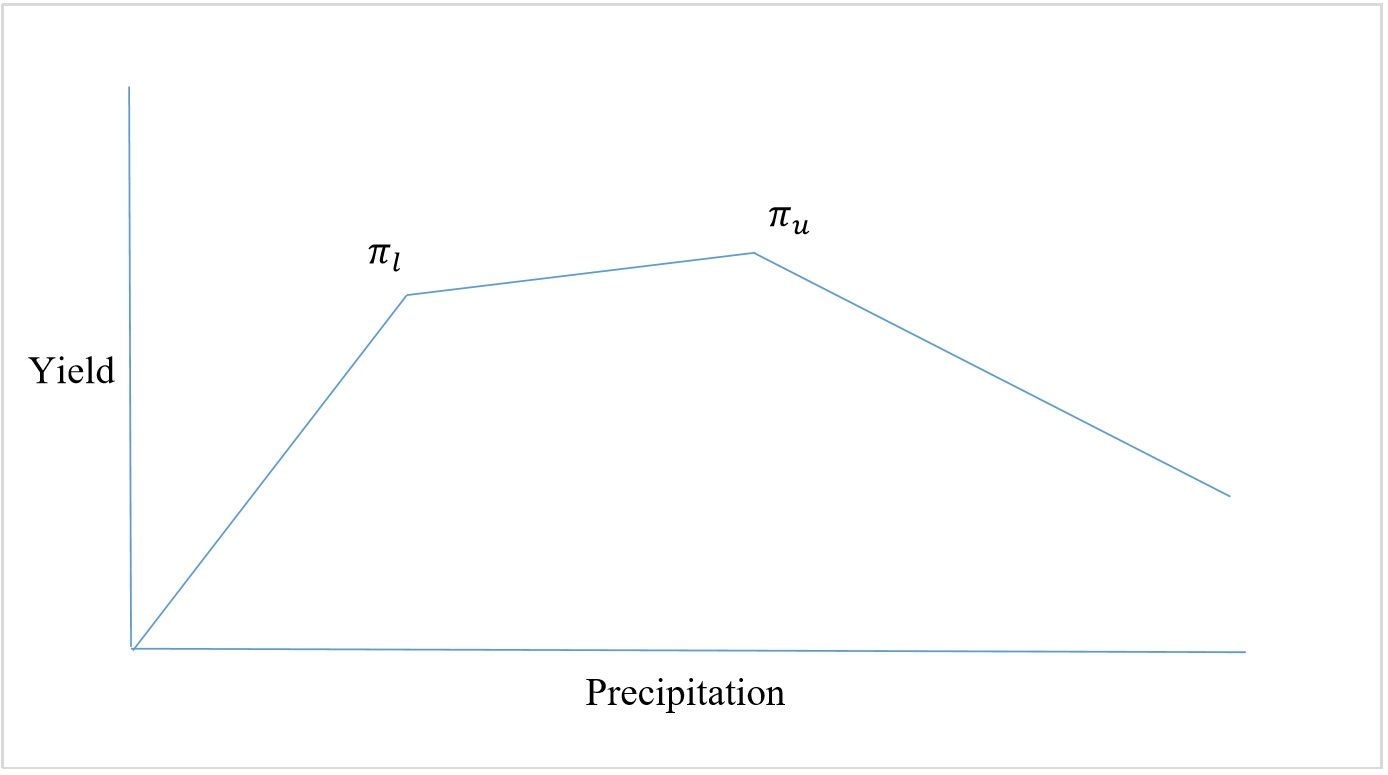
\includegraphics[width=\textwidth]{2threshold.jpg}
    \caption{Approximation of the yield precipitation relationship for use in empirical model}
 \end{figure}
    
In order to use this structure to consider the relationship between yield and precipitation, two additional precipitation variables which indicate when precipitation levels are above the lower and upper threshold values respectively, are included in the model. Precipitation demand is expected to have increased over time due to the increase in plants and yield per acre. Approximating the effect of precipitation on yields using a piecewise linear function as described above, this increased demand would be interpreted as increased lower and upper threshold levels. To allow for this in the empirical model, the threshold levels are allowed to change linearly through time.

\begin{equation}
\pi_l = a_l + b_lT
\end{equation}

\begin{equation}
\pi_u = a_u + b_uT
\end{equation}

Where $T$ represents time, $\pi_l$ is the lower threshold, $\pi_u$ is the upper threshold and $a_l,b_l,a_u,b_u$ are unknown parameters which determine the threshold levels at a given point in time. Finally, due to the large increases in expected yield during the period of study, a trend is included. In Iowa the yield over time appears to follow an approximately linear trend over the entire study period. In Ontario however it can be seen that yields began to rise more steeply beginning around year 2000.

    
\begin{figure}[!hb]
  \centering
  \begin{minipage}[b]{0.49\textwidth}
    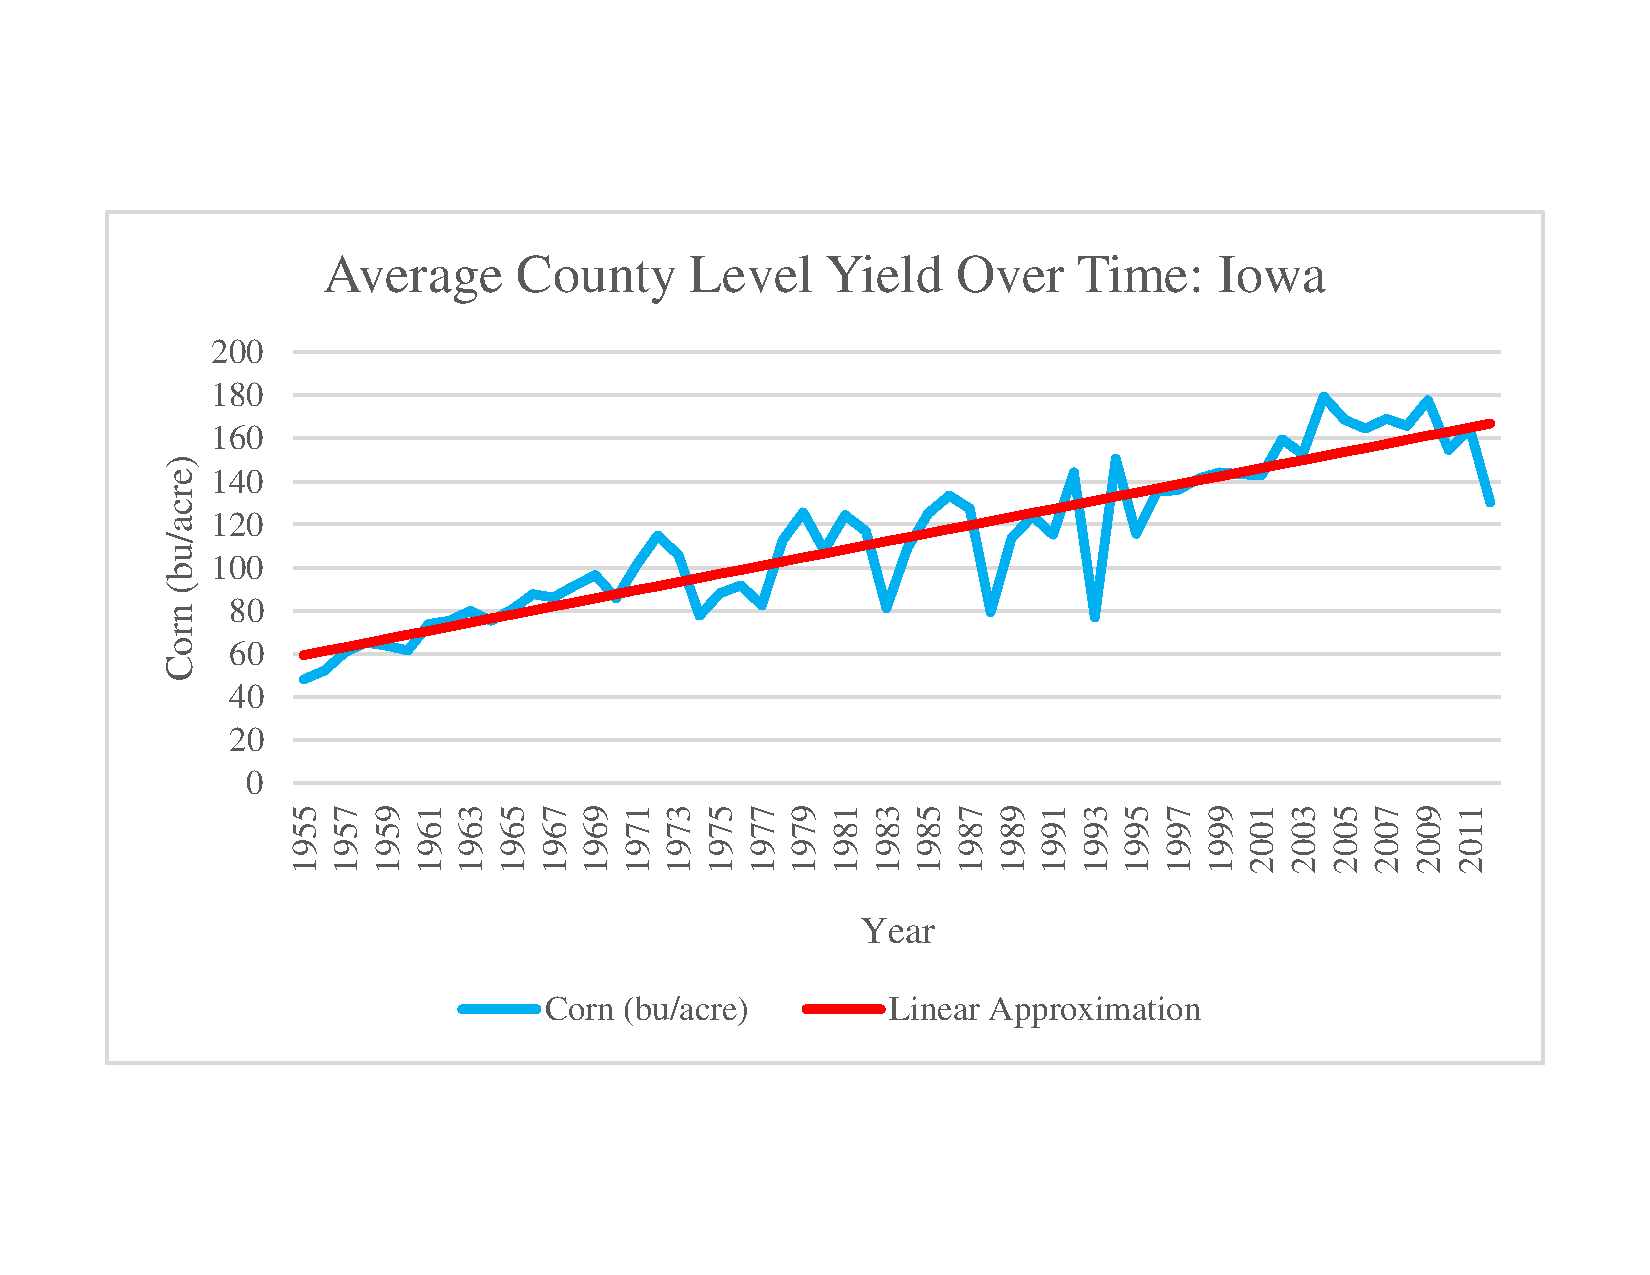
\includegraphics[width=\textwidth]{YieldIowa.pdf}
    \caption{Plot of Yield and Piece-wise Linear Approximation - Iowa}
  \end{minipage}
  \hfill
  \begin{minipage}[b]{0.49\textwidth}
    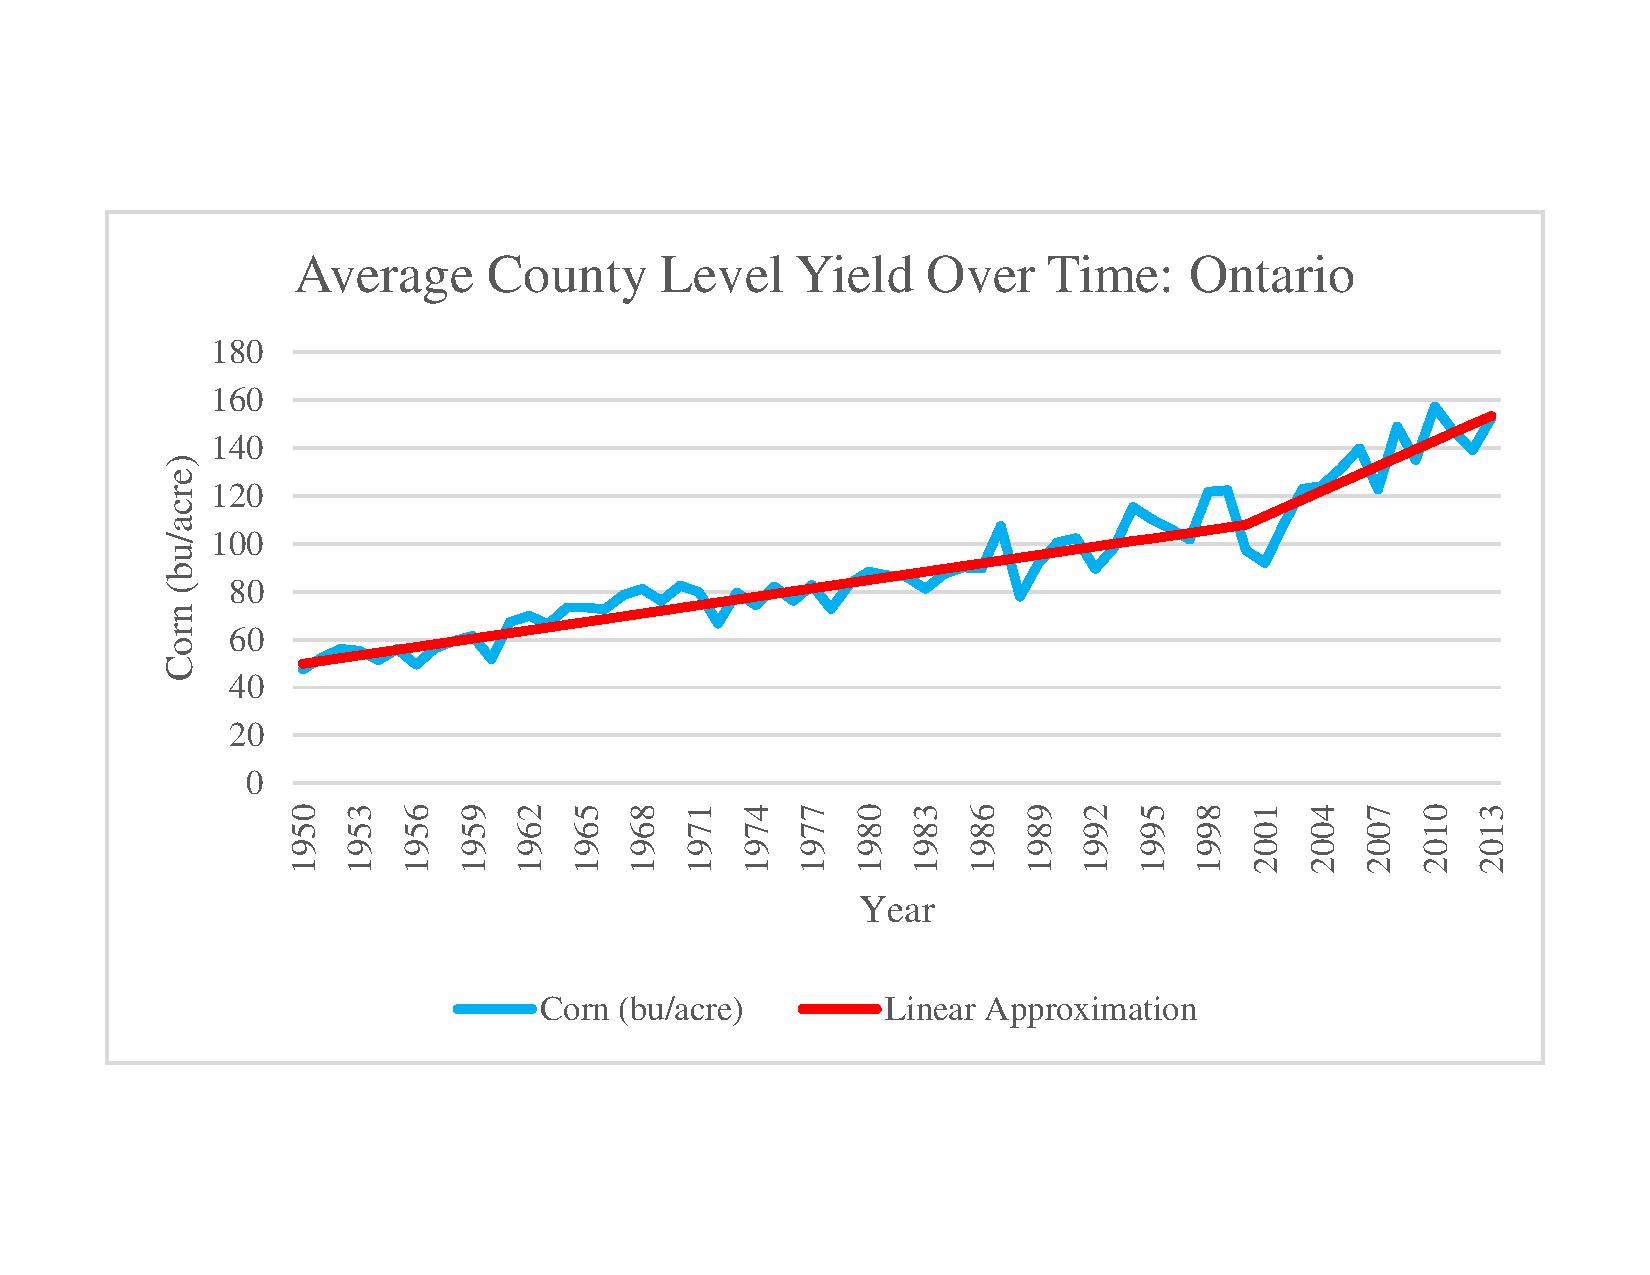
\includegraphics[width=\textwidth]{YieldOnt.pdf}
    \caption{Plot of Yield and Piece-wise Linear Approximation - Ontario}
  \end{minipage}
\end{figure}   
 
    
 Due to these observations, a single linear trend was included in the Iowa model, and a piecewise linear trend with a break point at 2000 in the Ontario model. This results in the following empirical models for Ontario and Iowa respectively:

\begin{equation}
Y=\beta_0+\beta_1p+\beta_2(max(PCP,\pi_u)-\pi_u)+\beta_3(max(PCP,\pi_h)-\pi_h)+\beta_4t+\beta_5(max(T,50)-50)+\delta X_{Ont}+\epsilon
\end{equation}

\begin{equation}
Y=\beta_0+\beta_1p+\beta_2(max(PCP,\pi_u)-\pi_u)+\beta_3(max(PCP,\pi_h)-\pi_h)+\beta_4t+\delta X_{Iowa}+\epsilon
\end{equation}

Where the $\beta$'s are scalar and unknown parameters, $\delta$ is a vector of unknown parameters, $t$ is the number of years since the beginning of the study period (1950 in Ontario and 1955 in Iowa), $X$ is a matrix of relevant weather variables in each location, and $\epsilon$ is an error term. The impact of omitted weather variables, as well as  of non-weather variables which affect yield, will be captured in the error term. A restriction on this model was also considered in which the upper and lower thresholds are equal to each other, thus collapsing to a single threshold model.

\section{Variable Choice}

An examination of the literature demonstrates that the choice of independent variables to include in the model is not trivial. Based on the results found in the literature review it appears that including a measure of vapour pressure deficit in addition to measures of precipitation and temperature can increase the fit of the model \citep{roberts2012agronomic}. Considering weather variables timed to growth stage has also been shown to increase the fit of the model as compared to averages over the growing season or monthly weather variables \citep{dixon1994estimating, ozkan2002impacts}. Schlenker and Roberts found that including the cumulative temperature over the growing season, by considering daily temperatures and modelling their distribution over each day, led to better results than using averages \citep{schlenker2009nonlinear}. A sin curve approximation of daily temperature distribution to calculate growing degree days will therefore be included. This variable is calculated using the method described in \cite{snyder1985hand}. 

Based on these results and on data availability, the following independent weather variables were considered for inclusion in the model:  accumulated and average precipitation, accumulated and average vapour pressure deficit, growing degree days, cold degree days, freezing degree days and extreme heat degree days. The timing of key growth stages was also considered so that the levels of the independent weather variables during each stage could be calculated. This was done due to account for changing relationships between yield and weather variables over the growing season. 

Precipitation is needed at a very low level in the initial growth stage. The crop water demand gradually increases throughout the vegetative stage as the plant progressively grows taller and develops more leaves \citep{OMAFRA}. Once all the leaves are developed the reproductive growth stages begin. Silks emerge from the corn plant and are receptive to pollination.  During this small period of time where pollen is being shed and silks have emerged the plant is very sensitive to environmental stress, such as drought or extreme heat \citep{OMAFRA}. The beginning of the silking and pollination stage is approximated by accumulated growing degree days (GDD) \cite{neild1987growing}. The GDD begin accumulating at the time of planting, and the various growth stages begin approximately after some particular GDD accumulation is reached. Unfortunately, a complete data set for planting days by county could not be found which made the determination of growth stage timing, and the subsequent creation of appropriate weather variables, difficult. The number of days to include within a particular growth stage is also somewhat unclear. For example, pollination takes about 7 days after the beginning of the silking period \citep{OMAFRA}, however, the exact amount of days will change from farm to farm. In order to increase the probability that the timed weather variables would capture the correct timing for most farms within the county, a few days were added on either end of the estimated beginning and end dates of the growth stage.

Given that the best method for timing growth stages is not clear, various timings and combinations of the variables were considered and tested in order to select the preferred set of independent variables for Iowa and Ontario respectively. On average silking and pollination occur at some point in July but the exact timing can vary based on environmental conditions.  Due to the difficulties involved in estimating the timing of growth stages, models with variables timed according to month were also considered. 

\section{Weather Data Timing}

As described above the weather variables were timed to particular stages of growth based on estimated planting dates and accumulated heat units. The heat units were measured using Growing Degree Days (GDD) in both Iowa and Ontario. The demand for precipitation is the relationship of interest and therefore the choice of how to time variables was especially focused on the agronomic yield-water relationship. As mentioned above precipitation has the most marked effect on yield when the corn plant is undergoing silking and pollination. Therefore estimation of the timing of the silking stage was the main focus.

In Iowa, access to a data set at the regional level identifying the percentage of corn acres which had been planted by each week between mid April and mid June was obtained. The data set also provided the percentage of acres where silking had begun by certain dates between early July and early August. Using this data set, the date at which 50 percent of corn acres had been planted in each region was calibrated. The resultant regional level 50th percentile date was then used as the planting date for each county within that region. The regional silking dates were calibrated in an analogous fashion. This data was available only for the years 1974-2012 with the exception of years 1987 and 1992, which only contained planting observations for 1 week in the season and were omitted. In order to estimate the planting and silking dates for the remaining years in the study, a linear model for planting dates was developed based on the planting and silking data described above. This model used weather in April as a predictor for planting date. Weather conditions in April were also used by \cite{gupta1985predicting} as an indicator of planting date. A trend was included in order to correct for the changes in farm management practices over time, which have generally led to earlier planting dates \citep{kucharik2006multidecadal}. The planting date model which was estimated was as follows:

\begin{equation}
  planting_{day}=\beta_0+\beta_1T+\beta_2Temp_{April}+\beta_3VPD_{April}+\beta_4PCP_{April}
\end{equation}

Where $Temp_{April}$ is the mean of the average daily temperature in April, $PCP_{April}$ and $VPD_{April}$ are averages of the daily precipitation and vapor pressure deficit totals in April, and $T$ represents time. This model was estimated using the calibrated county level planting dates for years 1974-2012 excluding 1987 and 1992.

The result of the planting date model estimation is shown below:



% Table created by stargazer v.5.2 by Marek Hlavac, Harvard University. E-mail: hlavac at fas.harvard.edu
% Date and time: Sun, Dec 11, 2016 - 8:42:16 PM
% Requires LaTeX packages: dcolumn 
\begin{table}[H] 
  \caption{Planting Date Model Results} 
  \label{} 
\begin{tabular}{@{\extracolsep{5pt}}lc} 
\\[-1.8ex]\hline 
\hline \\[-1.8ex] 
 & \multicolumn{1}{c}{\textit{Dependent variable:}} \\ 
\cline{2-2} 
\\[-1.8ex] & \multicolumn{1}{c}{planting\_day} \\ 
\hline \\[-1.8ex] 
 T & -0.310^{***} \\ 
  & (0.009) \\ 
 Temp$_{April}$ & -0.245^{**} \\ 
  & (0.098) \\ 
 VPD$_{April}$ & -12.567^{***} \\ 
  & (0.900) \\ 
 PCP$_{April}$ & 1.688^{***} \\ 
  & (0.084) \\ 
 Constant & 151.484^{***} \\ 
  & (0.664) \\ 
\hline \\[-1.8ex] 
Observations & \multicolumn{1}{c}{3,663} \\ 
R$^{2}$ & \multicolumn{1}{c}{0.485} \\ 
Adjusted R$^{2}$ & \multicolumn{1}{c}{0.484} \\ 
Residual Std. Error & \multicolumn{1}{c}{6.124 (df = 3658)} \\ 
F Statistic & \multicolumn{1}{c}{860.533$^{***}$ (df = 4; 3658)} \\ 
\hline 
\hline \\[-1.8ex] 
\textit{Note:}  & \multicolumn{1}{r}{$^{*}$p$<$0.1; $^{**}$p$<$0.05; $^{***}$p$<$0.01} \\ 
\end{tabular} 
\end{table} 

This model was used to predict planting date for the years in the study which were not included in the planting data set. For the years included in the planting data set, the calibrated planting and silking dates for each region were used for all the counties in that region. The planting dates resulting from this method were then used as  as the starting point for timing relevant growth stages.

 Planting data equivalent to that used for Iowa could not be accessed in Ontario. Given that there was no planting data, a planting date model could not be estimated. The method which has been favoured by OMAFRA for estimating planting date was used instead. This method assigns planting date to be the first day in the planting season where the previous 3 days have had average temperatures greater than or equal to 12.8 degrees Celsius \citep{OMAFRAhybrid}.

Since the warm weather variables HDD and GDD mostly attain positive values during the middle of the growing season (especially HDD) when they have the largest effect on the plant, seasonal totals of GDD and HDD were used to account for warm weather effects and the timing was not changed when testing the various models. Similarly, the cold weather variables are only likely to have non-zero values during the beginning and possibly end of the season, and were also not adjusted according to different timing methods.

Six different ways of timing variables were tested, and for each timing method 7 different combinations of the potential model variables were considered. Since Iowa and Ontario have slightly different climates and have different histories when it comes to corn production they were modelled separately. The different timings varied the amount of buffering added to the planting estimates, and also the number of subsets of growth stage that were considered. The details of the different timing options tested, and their agronomic significance, as well as the different combinations of variables considered are included in the  appendix in section 8.3.


\section{Estimation of Various Models for variable choice}

In order to select the variables which would be used in the model, several combinations of independent variables were considered. A linear yield model was estimated with each potential combination of independent variables and each timing method, and the resulting $R^2$ was stored. The choice of variables to include in the model for further analysis was determined based on the resulting adjusted $R^2$ from each model estimation, as well as on the interpretation of the model coefficients.

\subsection{Spatial Autocorrelation}

The model described in the empirical framework is a linear yield model based on weather variables and trend. In order to justify the estimation of this model using Ordinary Least Squares (OLS), the assumption that all of the observations are independent and identically distributed should hold at least approximately. Given the spatial nature of this data, the assumption of independence is hard to justify. Many unmeasured and unobserved variables such as soil moisture, soil temperature, seed hybrid, and choices relating to farm management affect yields. The effects of these excluded variables will be captured by the error term in the model. Some of these unobserved variables are determined by the local weather conditions which are certainly spatially correlated. Others relate to cultural norms and practices which are also likely to be correlated across space. This leads to the conclusion that the error terms in the model will most likely be spatially correlated. This is modelled as shown below, where X represents all variables included in the yield model including the constant term, trend and  precipitation effects:

\begin{equation}
y_{it}=X_{it}\delta+u_{it}
\end{equation}

\begin{equation}
u_{it}=\rho\sum_{j=1}^{n}(w_{ij}u_{jt})+\epsilon_{it}
\end{equation}

 The $i$ and $j$ subscripts are county indicators, while the $t$ subscript is a time indicator. Thus, $X_{it}$ is a row vector of explanatory variables for a given county and year. The error term $u_{it}$ from equation 3.7 depends on the errors from surrounding counties in that time period as shown in equation 3.8. The $w_{ij}$ terms are weighting terms which represent the effect of the error term in county $j$ on the error term in county $i$, $\rho$ is the spatial correlation parameter and $\epsilon$ is the uncorrelated vector of errors. It was assumed that counties with neighbouring borders would have spatially correlated errors. A symmetric spatial correlation matrix, $W$, was created based on the physical location of the counties in the study. The elements of this matrix were such that if counties $i$ and $j$ are neighbouring, $W_{ij}=1$, and if not, $W_{ij}=0$. This matrix was then row normalized. The interpretation of row normalization is that the degree to which any given county is affected by its neighboring counties is constant. In matrix notation the equation above becomes:


\def\kronecker{\raisebox{1pt}{\ensuremath{\:\otimes\:}}} 

\begin{equation}
Y= X\delta+u
\end{equation}

\begin{equation}
K=I_{T}\kronecker{W}
\end{equation}

\begin{equation}
u=\rho Ku+\epsilon
\end{equation}

This model is described in \citep{ord1975estimation}. $I_{T}$ is the identity matrix with dimension T by T, where T is the number of years included in the data set, and $K=I_{T}\kronecker{W}$ is the kronecker product of the T dimensional identity matrix with the spatial matrix $W$. The Kronecker product of two arbitrary matrices $A$, an n by m matrix, and $B$, a p by q matrix, is an np by mq matrix made up of pq block matrices, each of which is equal to the matrix $A$ multiplied by the element of matrix $B$ which corresponds to the relative position of the block matrix. Essentially the kronecker product of the T by T dimensional identity matrix with the N by N spatial matrix $W$ creates a spatial weighting matrix $K$ of dimension NT by NT which has non-zero values for neighbouring counties in the same time period and zero's elsewhere. Thus this model allows for correlation only between neighbouring counties, and no correlation over time. If the correlation coefficient $\rho$ is known, this model can be reconfigured in the following way such that least squares estimation is feasible:

\begin{equation}
A=I_{NT}-\rho K
\end{equation}

\begin{equation}
u-\rho Ku=\epsilon=Au
\end{equation}

\begin{equation}
Y- X\delta=u
\end{equation}

\begin{equation}
    A(Y- X\delta)=Au=\epsilon
\end{equation}

\begin{equation}
    AY=AX\delta +\epsilon
\end{equation}

\begin{equation}
    Y_{new}=AY
\end{equation}

\begin{equation}
    X_{new}=AX
\end{equation}

\begin{equation}
    Y_{new}= X_{new}\delta+\epsilon
\end{equation}

Equation 3.19 can now be estimated by OLS on $Y_{new}$ and $X_{new}$ yielding:

\begin{equation}
  \delta=(X_{new}^TX_{new})^{-1}X_{new}^TY
\end{equation}

On the other hand, if $\delta$ is known, $\rho$ can be estimated using the method of maximum likelihood. Given that $\epsilon\sim N(0,\sigma^2I_{NT})$ and $Au=\epsilon$ it follows that:

\begin{equation}
    u=A^{-1}\epsilon
\end{equation}
\begin{equation}
    u\sim N(0,A^{-1}\sigma^2A^{-1T})
\end{equation}

Therefore, the probability density function for $u$ is as follows:

\begin{equation}
    f(u)=\frac{|A|}{\sqrt{(2\pi)^{NT}\sigma^2}}e^{\frac{-1}{2\sigma^2}u^TA^TAu}
\end{equation}

Which gives the following log likelihood equation:

\begin{equation}
  L(u)=ln(f(u))=ln(\frac{1}{\sqrt{2\pi\sigma^2}})+ln(|A|)-\frac{1}{2\sigma^2}u^TA^TAu
\end{equation}

This equation can then be maximized with respect to $\rho$, given that $\delta$ is known. The estimation method was developed based on the method from \cite{cochrane1949application}. In \cite{cochrane1949application} an iterative estimation procedure is developed whereby least squares is applied naively to $Y$ and $X$ in order to generate an estimate of $\delta$, which is used to estimate $u$. The estimate of $u$ is then used to estimate $\rho$. The estimate of $\rho$ is then used to re-estimate $\delta$ which is then used to re-estimate $u$. The process is continued until the desired level of convergence is attained. However, since $\delta$ is dependent only on known $X$ and $Y$ and unknown $\rho$, the equation for $\delta$ can be subbed into the likelihood equation, creating an equation in only one variable which can then be maximized directly for $\rho$. The value of $\delta$ can then be solved for  immediately. Thus the model can be estimated by the maximization of the likelihood function with respect to $\rho$, when neither $\rho$ nor $\delta$ is known. 


\subsection{Unknown Threshold Levels}

In the empirical model section the use of threshold levels which change through time to model the potentially dynamic effect of precipitation on yield over the study period was described. The appropriate threshold levels are unknown, and therefore need to be estimated. In the two threshold case the threshold levels are determined by four parameters, $a_l$, $b_l$, $a_h$, and $b_h$. Thus, four parameters must be estimated in order to determine optimal thresholds over time. In order to approach this problem vectors of possible values within appropriate constraints were chosen for each of the four parameters. Each possible combination of the values in these four vectors was considered, and the model was estimated given thresholds determined by that particular parameter combination. The model SSE was stored, and the combination of the four parameters leading to the lowest SSE was selected as the optimal estimate. In the one threshold model only two parameters need to be determined but the procedure is analogous to that described above. Since there are four and two dimensions of unknown parameters respectively this process was very computationally demanding, and therefore was infeasible to do for each combination of variables being considered for the model. For this reason, the threshold variables were omitted when estimating the models in order to determine variable choice. 

\subsection{Results of Model testing for variable choice}

After estimating each model for Iowa and Ontario respectively, the results were considered in terms of SSE and additionally in terms of the sign and significance of the coefficients. The variance of the model coefficient estimates are approximated using robust standard errors. As discussed in the data section, access to planting and silking data in Ontario could not be obtained, and therefore the planting dates were estimated based only on temperature. This was likely a much less accurate way of estimating planting dates than what was used in Iowa. In Iowa, the selected model timed precipitation and vapor pressure deficit to growth stages according to the planting date model coupled with accumulated growing degree days. In Ontario however, the model which included monthly precipitation and vapor pressure deficit outperformed the model which timed variables to approximate growth stages.  This result could be due to the difference in ability to accurately time growth stages in Ontario and Iowa.

In Ontario the model chosen was $d_{iii}$. Timing iii divides the growing season by month as opposed to by timed growth stages. The precipitation and vapor pressure deficit variables are the cumulative totals for each month from May to August. The heat variables included in this model are growing season accumulated GDD and HDD. In Iowa the model chosen was $d_{iv}$. Timing iv breaks up the growing season into 3 stages corresponding to a beginning of season stage, a pollination stage and an end of season stage. The timing of the variables relative to the estimated planting and silking dates is shown below: 

$$\text{Precipitation for beginning of season stage: }PCP_{b_i}=sum(PCP[\text{planting:silking-14}])$$
$$\text{Precipitation for pollination stage: }PCP_{pol_i}=sum(PCP[\text{silking-13:silking+14})$$
$$\text{Precipitation for end of season stage: }PCP_{e_i}=sum(PCP[\text{silking+15:maturity}])$$

The vapor pressure deficit variables are created in the same manner and using the same dates for timings as the precipitation variables. Descriptions of the different timing options and their relation to agronomic growth stages is included in the appendix section 8.3, as is a comprehensive list of the model testing results for all timings and combinations of variables in both Iowa and Ontario.

\section{Estimation of model including dynamic thresholds}

In the empirical model, threshold levels for the precipitation variable are included. The models chosen for both Iowa and Ontario include multiple measures of precipitation corresponding to different periods of the growing season. Given that precipitation is most important, in terms of yield effects, during the silking and pollination stage, the thresholds were included for the precipitation variable which was most closely timed to this period. In Ontario this was the July precipitation variable, while in Iowa it was the precipitation variable timed to silking stage. As noted in the previous sections, four unknown parameters control the values of the upper and lower thresholds in the two threshold case while two parameters control the value of the threshold in the single threshold model. A direct search method was used to determine the best choice for these parameters where a function which output the model SSE for a given vector $x$ of these four parameters, $x=(a_l,a_h,b_l,b_h)$, was used. Vectors of values which each of these parameters could take on were created. The vectors of potential values were constructed such that the lower and upper threshold could never overlap. The upper threshold was also constrained to be smaller than the maximum precipitation level obtained in the study period. Similarly the lower threshold was constrained such that it was above the minimum precipitation level received in the study period for all years. Every combination of the values in these four vectors was then tested, and the SSE of the model given those values was determined and saved. The combination of the four parameters which led to the lowest resultant SSE was selected. An analogous method was used for the single threshold model estimation, with two parameters as opposed to four.

\chapter{Historical Data Modelling Results}
The yield model results with optimal threshold levels, as well as the estimated values of the threshold parameters, will be presented. The relationship between precipitation and yield during the approximate time where silking and pollination occurs was modelled  as a piecewise linear function. This relationship was modelled with two separate threshold points. The constrained case where the second threshold coefficient is set equal to the first, thereby collapsing the model to a single threshold model was also considered. Spatial autocorrelation was dealt with using a spatial weighting matrix which indicates neighbouring counties' observations within the same time period. The spatial correlation parameter $\rho$ was estimated by maximizing a likelihood function with respect to this parameter. As the maximizing value can not be exactly solved algebraically, this maximization was accomplished using the optim function in R, but could also be done through a direct manual search on potential values of $\rho$. The maximization of the likelihood function needed to determine the optimal spatial correlation parameter $\rho$ for a particular model is very time consuming. Two method variations were considered for the estimation of the yield models. The first method assumes that the optimal value for the spatial correlation parameter would depend on the threshold levels. In this method the optimal spatial correlation parameter was recalculated for every combination of threshold parameters considered. This method is very computationally expensive, as the likelihood function must be optimized for $\rho$ given each potential set of threshold parameters, and limits the number of different parameter combinations that can be tested. The second method assumed that the threshold levels would not have a significant effect on the optimal spatial correlation parameter. The optimal spatial correlation parameter was estimated with the threshold variables omitted; this value was then used for the model estimation given each combination of threshold parameters considered. This was done to consider how robust the results would be to a simplification of the model which significantly decreased computing time. Each method was used to estimate the optimal threshold parameters for both the one and two threshold models. This led to four different results for the optimal threshold estimates in each location. The first result was from the method 1 estimation of the two threshold model, the second was from the method 2 estimation of the two threshold model, the third is from the method 1 estimation of the one threshold model, and the fourth is from the method 2 estimation of the one threshold model. Therefore, four results are reported for each location subset with heteroskedastic consistent errors generated using the HC3 option of the hccm function in R. 


\section{Ontario Sub Sections}


Ontario has a varied history of corn production throughout the province and significant climatic differences between the counties included in the study\citep{tolhurst2015cold}. Due to the presence of between county heterogeneity in Ontario, a single model may not be sufficient to accurately describe corn production for all counties included in this study. In general, the following counties: Brant, Chatham-Kent, Elgin, Essex, Haldimand-Norfolk, Lambton, Middlesex and Oxford, in Southern Ontario, have historically had higher average yields in comparison to other counties in the province. These counties are also in close physical proximity to one another. This physical proximity is likely linked to similarities in  farm management practices as well as environmental conditions (for example soil moisture) which are not reflected in the available weather data. These omitted variables are likely to affect yield. On the other hand, certain counties spread throughout the province which were included in our data set have have had relatively low average yields throughout the study period. These counties are Dufferin, Grey, Halton, Hamilton, Hastings, Kawartha Lakes, Lanark, Leeds-Grenville, Lennox-Addington, Niagara, Northumberland, Prince Edward and Renfrew. A ``Corn Producer" subset of Ontario counties was therefore considered in which the counties in this list were excluded. Figure 4.1 shows the average yield over time of all counties in our data set (``All Counties"), the 8 counties included in the Southern Ontario group (``Southern Ontario"), the group of counties with the lowest producers excluded (``Corn Producers"), and the 13 other counties with lower average yield (``Low Producers"). 


\begin{figure}[H]
\centering
 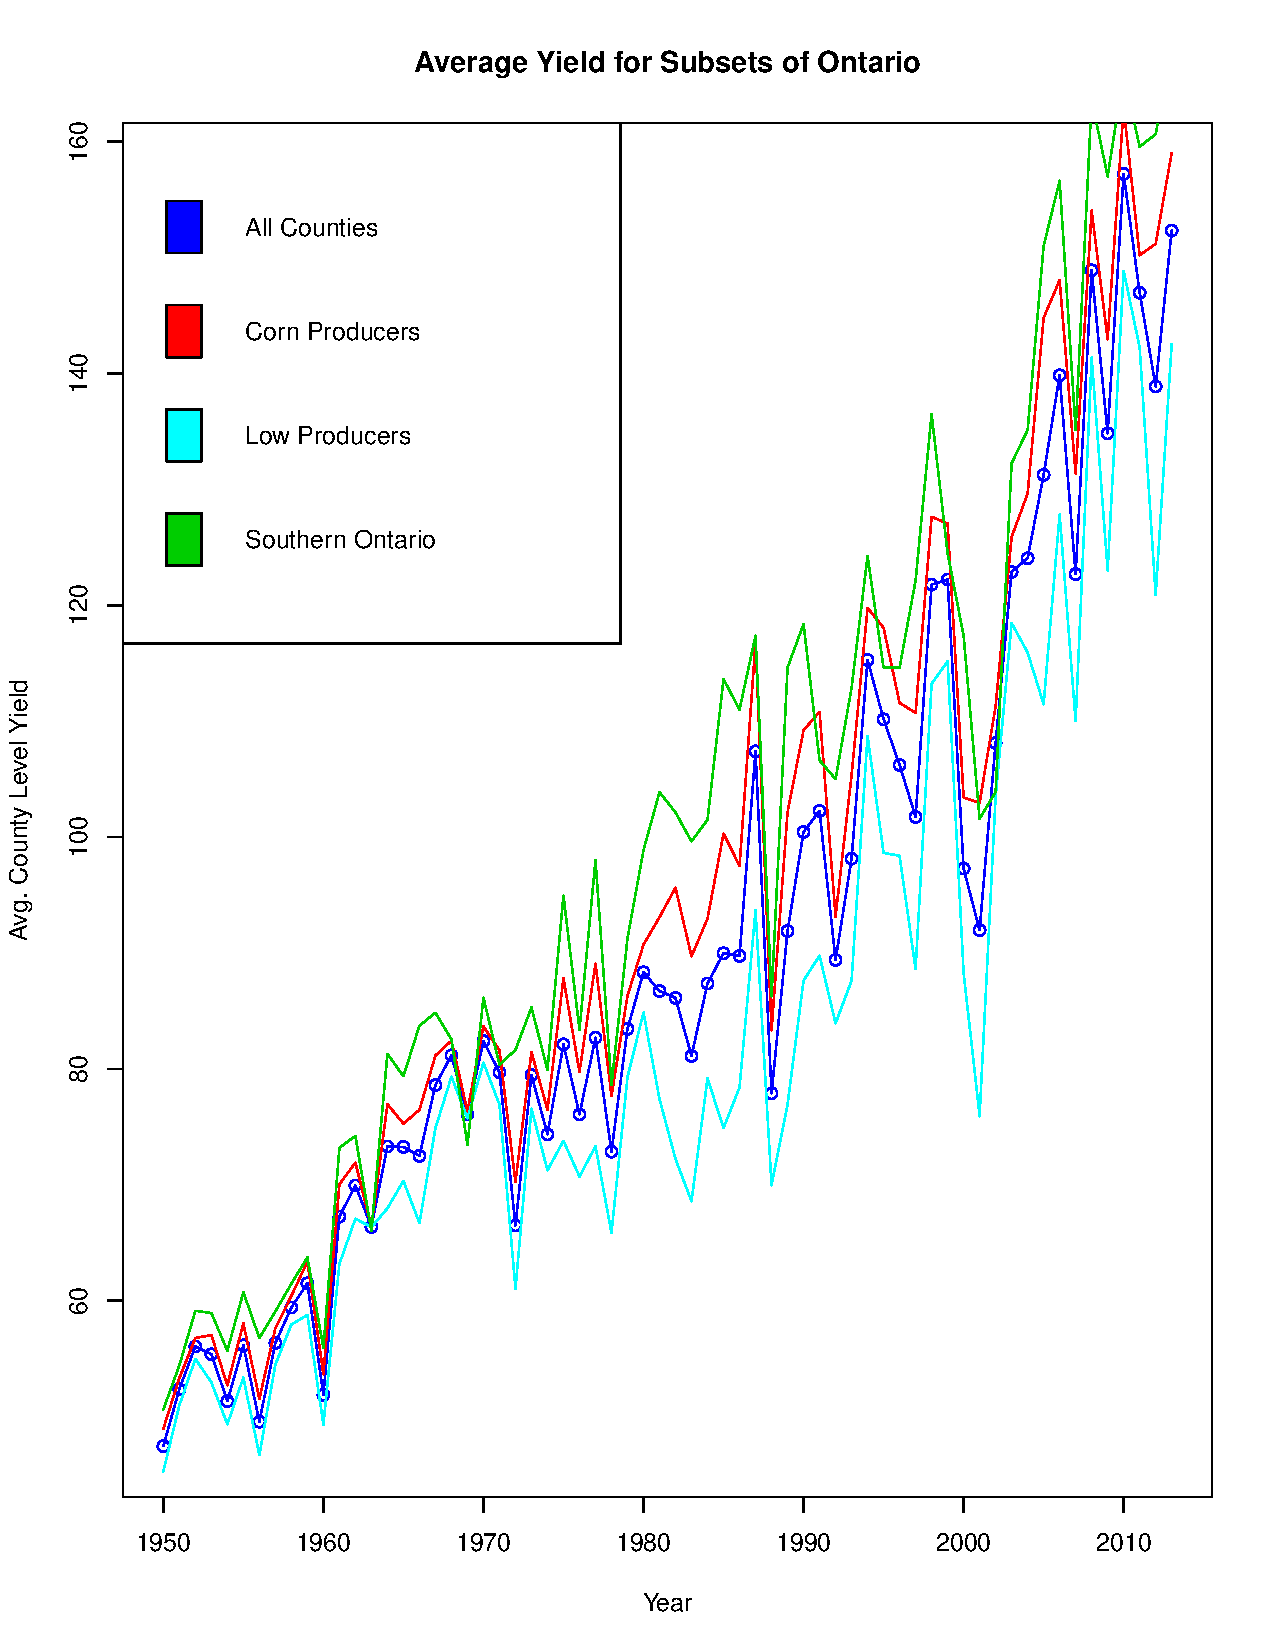
\includegraphics[width=.95\textwidth]{YieldsON.pdf}
    \caption{Plot of Average County level Yield for Subsets of Ontario}
    \end{figure}


Due to the differences in the average county level yields between groups, the yield models were estimated on the ``Southern Ontario" and ``Corn Producers" subsets, in addition to the group including all counties. Another concern results from the climate data used in Ontario. This data comes from environment Canada and was spatially interpolated to county center points. Environment Canada has radar stations spread throughout the province with only 8 radar stations covering the province \citep{EnvirCan}. The counties nearest to these radar stations could have more accurate weather data than the other counties due to this proximity, and could therefore demonstrate the yield climate relationship with higher accuracy. The modelling and determination of threshold levels using only counties nearest to these radar stations was also considered. The counties in question were the following: Huron, Middlesex, Ottawa, Peel, Perth, Prescott-Russel, Stormont-Dundas-Glengarry and York. Results will be presented for the four methods of determining threshold levels for each of these four groups: the entire set of counties, the counties in Southern Ontario, the counties closest to radar stations (``Weather Station Counties"), and the group of counties excluding the 13 less substantial producers. A table will present the relevant regression results for each group.

Iowa is relatively homogeneous in comparison to Ontario. Although there are some climate differences in different regions in the state, most of the counties have been significant producers of corn historically, and Iowa is therefore not subject to the same degree of heterogeneity that Ontario is. All of the counties in Iowa are included in the same model.

\section{Model Results}

The tables below present the model estimates for each location. The model results are from the OLS estimation performed on the transformed data, $Y_{new}$ and $X_{new}$ described in chapter 3, and are presented with robust standard errors (generated using method HC3 in the hccm package in R). In the Ontario model, county specific dummy variables were included, while in Iowa, region specific dummy variables were included. The parameter estimates for these variables are excluded from the tables below for the sake of space.


\begin{table}[H]
    \centering
    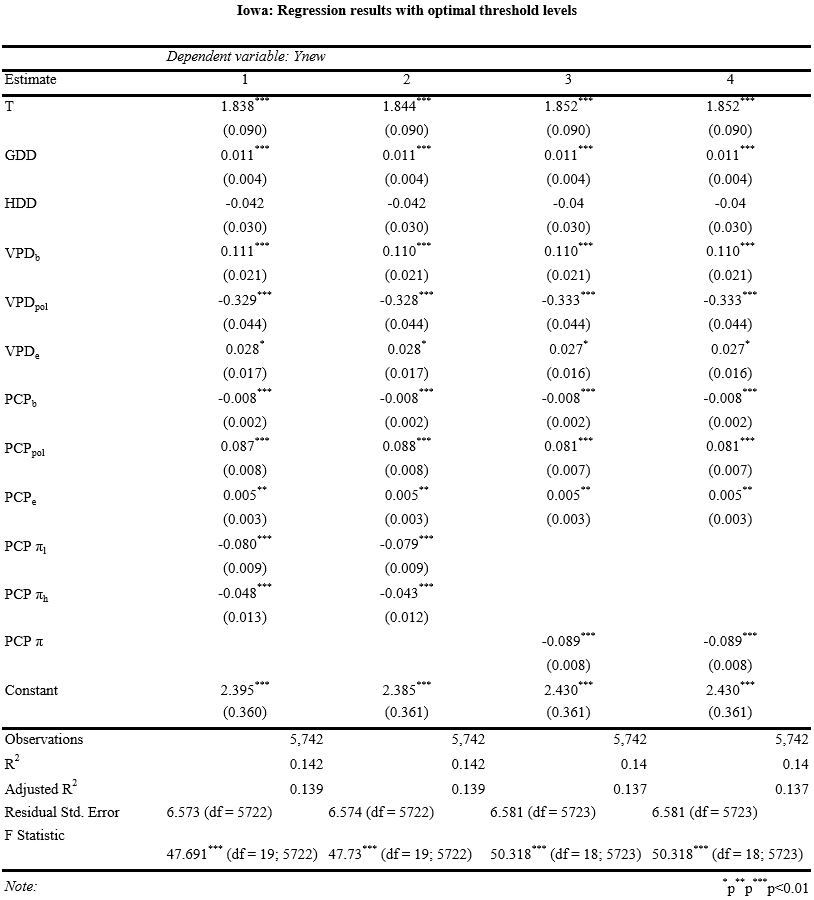
\includegraphics[width=1.0\textwidth]{Iowa_regression_results.png}
    \caption{Iowa: Regression results with optimal threshold levels}
    \label{fig:my_label}
\end{table}

\begin{table}[H]
    \centering
    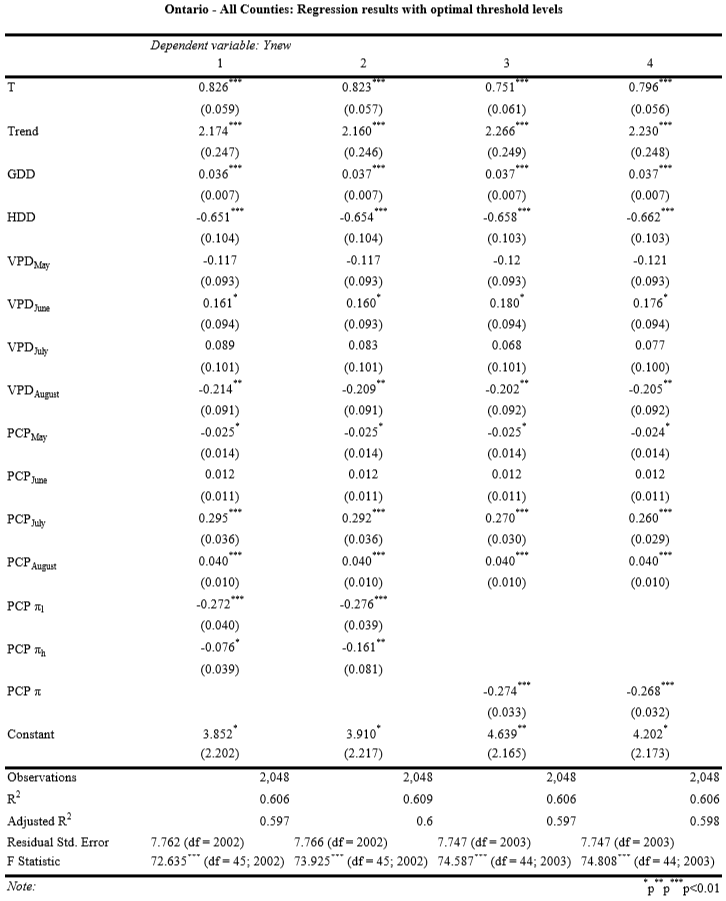
\includegraphics[width=1.0\textwidth]{Ontario_regression_results.png}
    \caption{Ontario - All Counties: Regression results with optimal threshold levels}
    \label{fig:my_label}
\end{table}

\begin{table}[H]
    \centering
    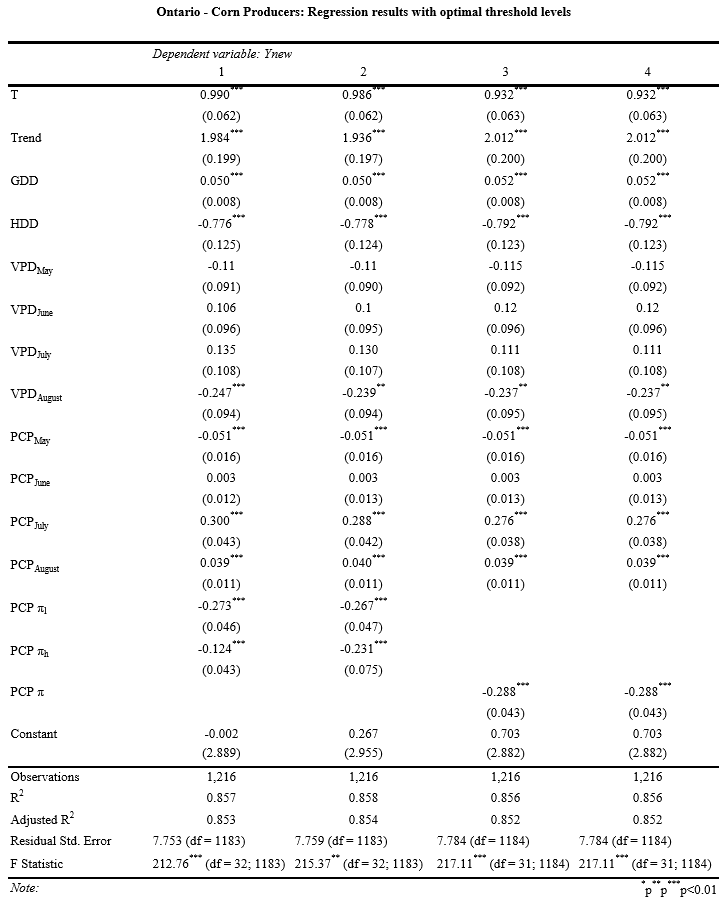
\includegraphics[width=1.0\textwidth]{Ontario_trim_regression_results.png}
    \caption{Ontario - Corn Producers: Regression results with optimal threshold levels}
    \label{fig:my_label}
\end{table}


\begin{table}[H]
    \centering
    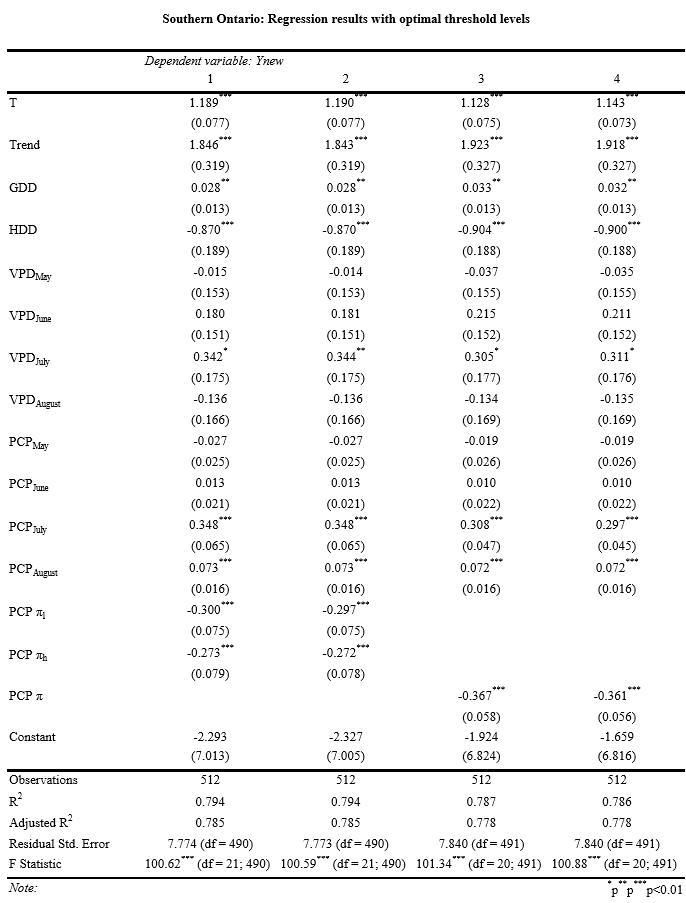
\includegraphics[width=1.0\textwidth]{Ontario_SO_regression_results.png}
    \caption{Southern Ontario: Regression results with optimal threshold levels}
    \label{fig:my_label}
\end{table}


\begin{table}[H]
    \centering
    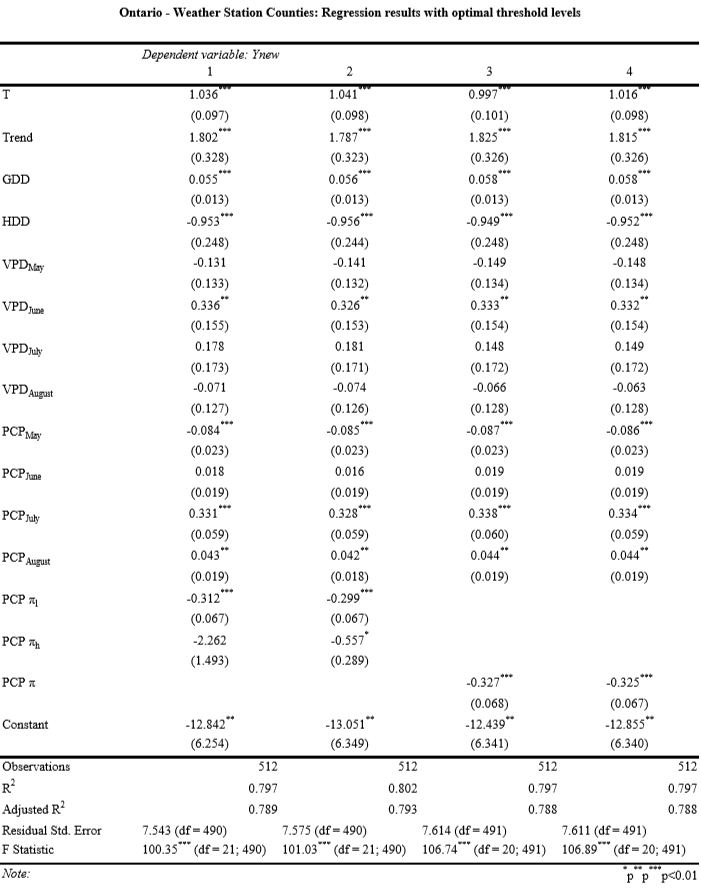
\includegraphics[width=1.0\textwidth]{Ontario_WSO_regression_results.png}
    \caption{Ontario - Weather Station Counties: Regression results with optimal threshold levels}
    \label{fig:my_label}
\end{table}

The model results from Iowa demonstrate the expected signs on all of the coefficients. The trend variable has a positive coefficient estimate as does GDD, while HDD, the variable representing potentially damaging high temperatures, has a negative coefficient with large magnitude. The Vapor Pressure Deficit (VPD) measure used is based on the difference between the saturated vapor pressure level at the maximum and minimum daily temperatures respectively. When the VPD levels are high, it indicates hot and dry conditions. Warm temperature with little moisture during planting and the early growth stages is generally beneficial for corn growth.  On the other hand, during the silking and pollination period crops are sensitive to extreme heat and water loss. During the end of the season the majority of growth is completed and the temperatures are becoming cooler. This leads to the expectation of a positive coefficient on beginning of season VPD, a negative coefficient on VPD during silking and pollination and a positive coefficient during the end of the season. All four of the results demonstrate these expected relationships in Iowa. The precipitation effect also changes throughout the growing season. In all four results, the sign on the $PCP_b$ variable, which corresponds to the beginning of the season when high levels of moisture can be damaging, is negative and small. During the silking stage the precipitation coefficients become positive and larger in magnitude which is consistent with the high levels of moisture required during this period. Finally, the end of season precipitation variable, $PCP_e$, is small and positive. Additionally, the silking stage precipitation threshold variable coefficients are both negative, as expected, given that the positive effect of precipitation in excess of the first threshold is expected to be small, and the effect of precipitation in excess of the second threshold is expected to be negative. Therefore, all of the coefficients are in the expected direction for all of the model estimates in Iowa. 

In the results for the province of Ontario and the three subsets considered, all of the coefficients had the expected signs except for the VPD coefficients. Otherwise, as in Iowa, the expected relationships are observed. In particular, the precipitation coefficients in July and the threshold coefficients have the expected signs and relative magnitudes. The general predicted yield climate relationship in Ontario and its subsets were very similar. Although the $R^2$ was higher among the smaller groups of counties which had more similarities, the general relationship was consistent across all of the models in terms of the sign and magnitudes of the parameter estimates. Given this observation, the remaining analysis is done only in reference to the group including all counties, and the subsets of the province are not considered further as they did not suggest a substantial difference in the effect of yield on climate by location.

\section{Precipitation Coefficient Estimates}

The precipitation coefficients are graphed versus precipitation level to demonstrate the implied effect of precipitation on yield. The coefficients are presented relative to the optimal threshold levels in 2000. The coefficient estimates obtained under each model and method are graphed together for each location.


\begin{figure}[H]
\centerfloat
 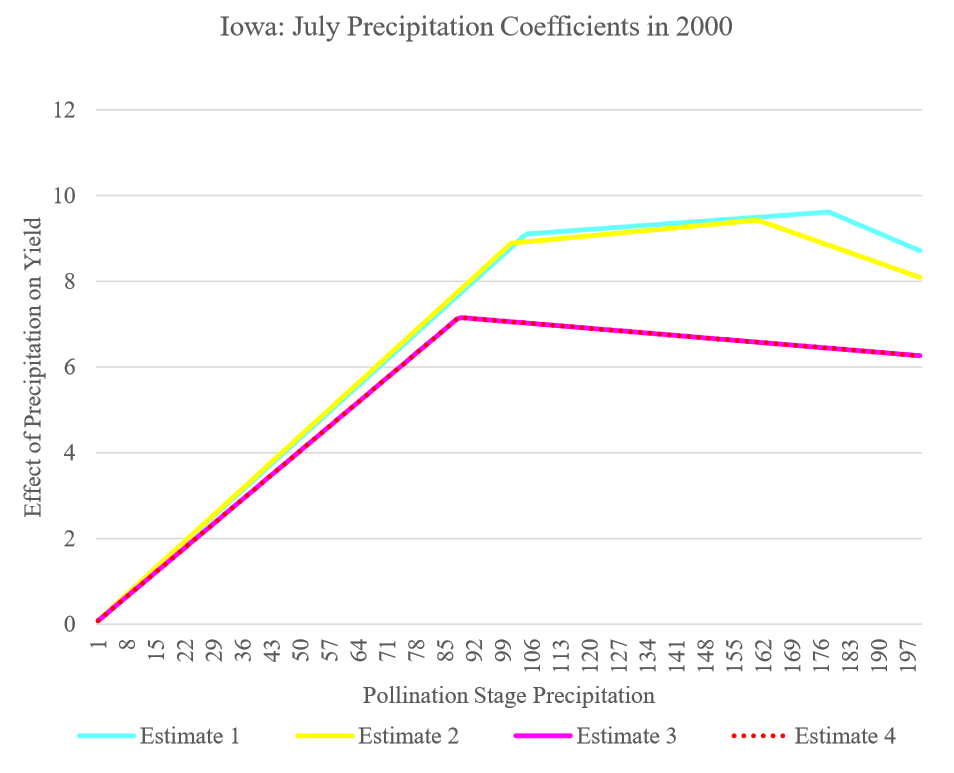
\includegraphics{Iowa_coefs.png}
    \caption{Iowa: Plot of Silking Stage Precipitation Coefficients using Threshold Levels from 2000}
\end{figure}

\begin{figure}[H]
 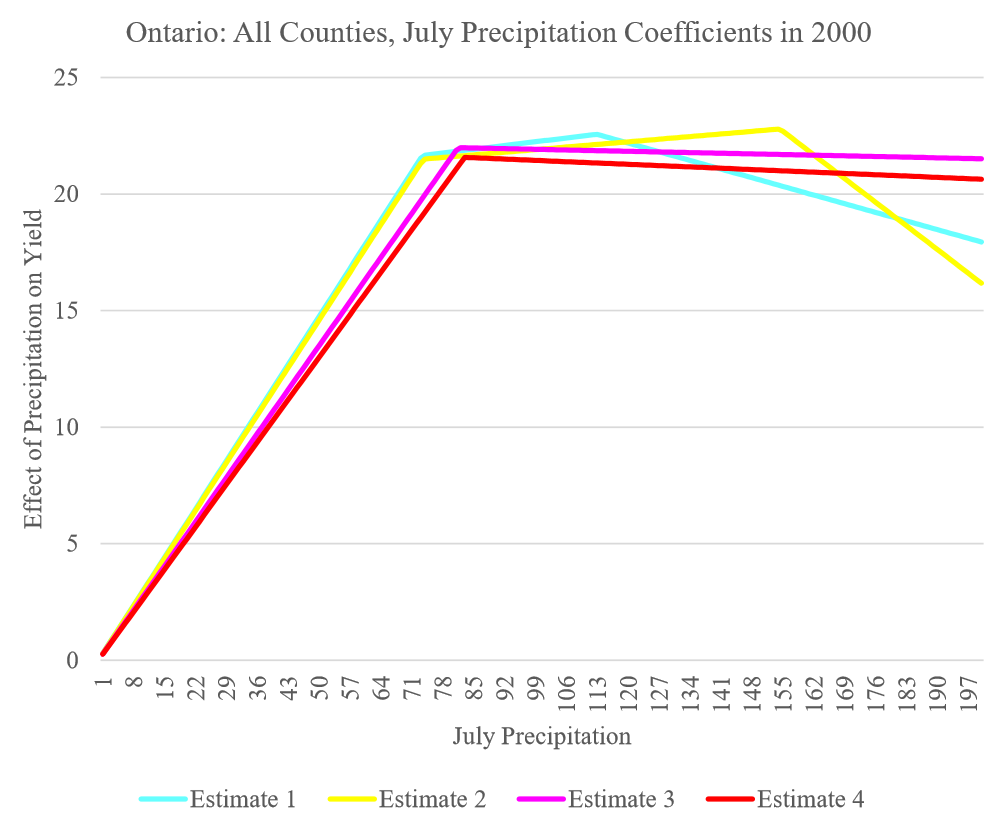
\includegraphics[width=\textwidth]{ON_coefs.png}
    \caption{Ontario: All Counties - Plot of July Precipitation Coefficients using Threshold Levels from 2000}
\end{figure}


\begin{figure}[H]
\centerfloat
 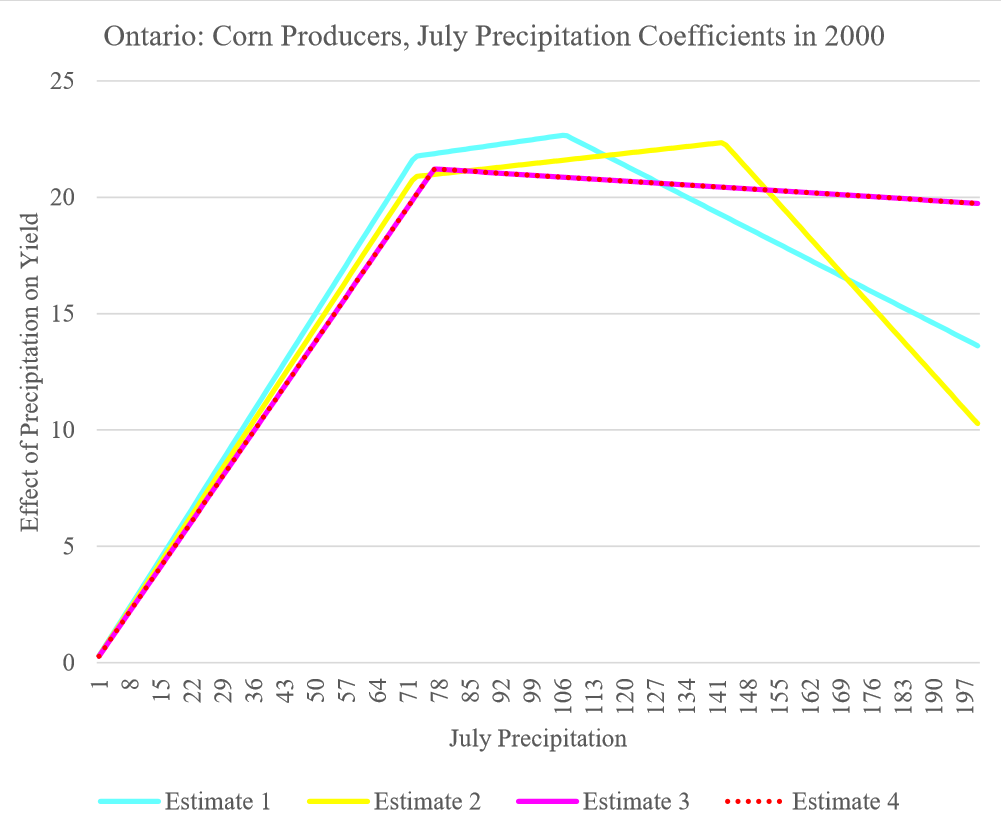
\includegraphics{trim_coefs.png}
    \caption{Ontario: Corn Producers - Plot of July Precipitation Coefficients using Threshold Levels from 2000}
\end{figure}

\begin{figure}[H]
\centerfloat
 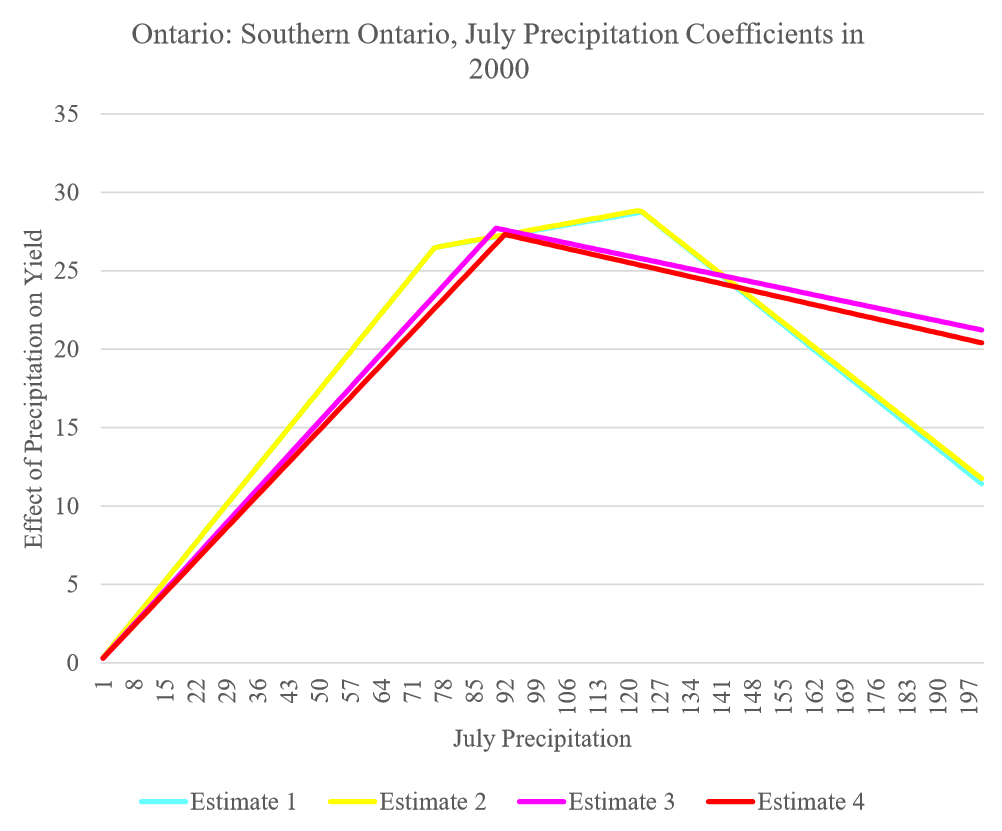
\includegraphics{SO_coefs.png}
    \caption{Southern Ontario - Plot of July Precipitation Coefficients using Threshold Levels from 2000}
\end{figure}

\begin{figure}[H]
\centerfloat
 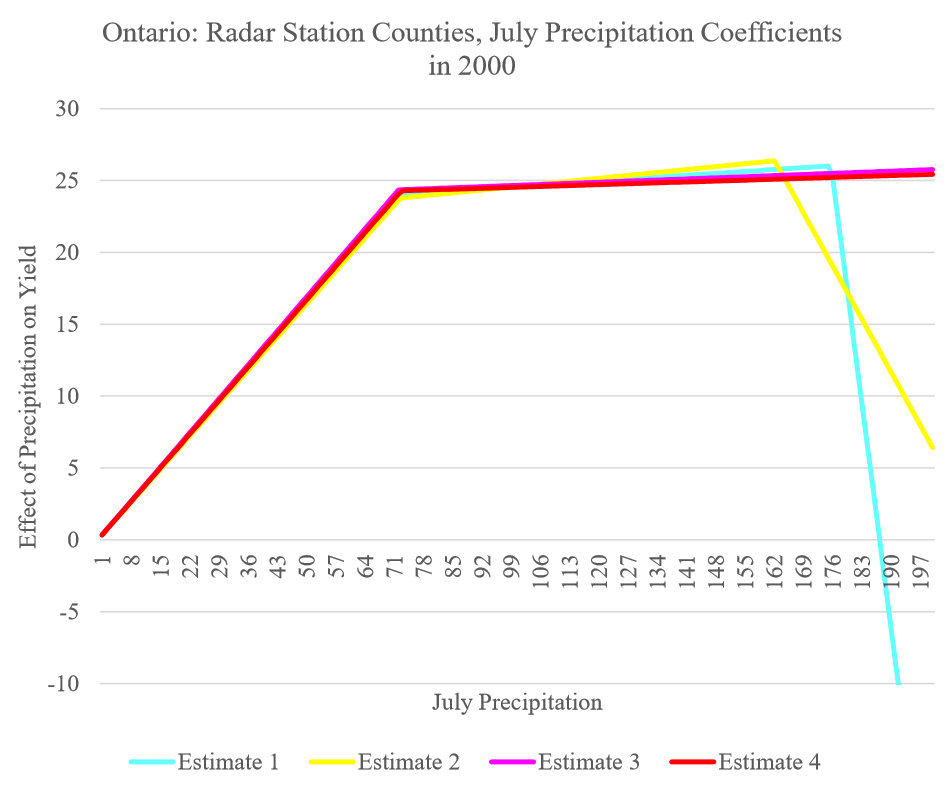
\includegraphics{WSO_coefs.png}
    \caption{Counties Near Ontario Radar Stations - Plot of July Precipitation Coefficients using Threshold Levels from 2000}
\end{figure}


The graphical presentation of the coefficients on silking stage precipitation levels demonstrates that they are consistent with the theoretical precipitation yield relationship. In all of the two threshold cases the implied effect of precipitation on yield, based on the estimated coefficients, is shown to be positive for small amounts of precipitation, then to start to level off after the first threshold, and finally to become negative after the second threshold. In the one threshold cases the implied effect begins positive and then decreases after the threshold level has been exceeded. These results fit well with the empirical framework that was developed, and fulfill the intuitive expectations regarding the effect of precipitation on yield during the silking and pollination stage.

\section{Threshold Results}

The optimal parameters controlling threshold levels estimated under each method and for each location are presented in the table below. 


\begin{table}[H]
\caption{Threshold Parameter Results by Location}
\label{my-label}
\begin{tabular}{lllllll}
\hline
 & $a_l$ & $b_l$ & $a_h$ & $b_h$ & $a$ & $b$ \\
\hline
 Iowa & & & & & & \\
\hline
1  & 60.416  & 0.982759   & 345.1  & -3.71379    &  & \\
2  &  64.416 & 0.813793  & 288.1         & -2.83103     & &   \\
3  &  &   &          &      & 86.416 &   0.434483 \\
4   &  &   &          &      & 86.416 &   0.434483 \\
\hline
Ontario: All counties & & & & & & \\
\hline
1  & 12 &  1.228125   & 137.25   &  -0.4875    &  & \\
2  &  13 & 1.2125  & 121.25         & 0.6625     & &   \\
3  &  &   &          &      & 3 &  1.56875 \\
4   &  &   &          &      & 10 &   1.4593753 \\
\hline
 Ontario: Corn Prducers & & & & & & \\
\hline
1  & 8 &  1.290625   & 140.99    &  -0.6875   &  & \\
2  &  8 & 1.290625  & 121.99      & 0.409375     & &   \\
3  &  &   &          &      & 5 &  1.4375 \\
4   &  &   &          &      & 5 &   1.4375 \\
\hline
 Southern Ontario & & & & & & \\
\hline
1  & 30.18 & 0.91875   & 118.37    &  0.09375   &  & \\
2  &  30.18 & 0.91875  & 116.37     & 0.125     & &   \\
3  &  &   &          &      & 32.18 &  1.15625 \\
4   &  &   &          &      & 34.18 &   1.15625 \\
\hline
Ontario: Radar Station Counties & & & & & & \\
\hline
1  &  10.06 & 1.253125   & 148.2    &  0.55    &  & \\
2  &   9.06 & 1.26875  & 132.2     & 0.6      & &   \\
3  &  &   &          &      & 7.06 &  1.3 \\
4   &  &   &          &      & 10.06 &    1.253125 \\
\hline
\end{tabular}
\end{table}



As shown in table 4.1, the results from the two threshold model in Iowa show that the lower threshold appears to be increasing through time while the upper threshold is decreasing. This result was found when the two threshold model was estimated both by method 1 and 2. The one threshold model results both showed the single knot to be increasing. 

The threshold results for all counties in Ontario generally show increasing thresholds over time. Estimate 1 shows a decreasing upper threshold over time, however, estimate 2 shows the upper threshold to be increasing. The one threshold model results both show the threshold to be increasing through time. The results for the ``Corn Producer" subset were very similar to those obtained for the entire province. The results for other two provincial subsets, ``Southern Ontario" and ``Weather Station Counties", showed all thresholds to be increasing under both models, and both estimation methods.

 The one threshold dynamic model results consistently showed that the precipitation threshold was increasing over time in all locations, and when estimated using both methods 1 and 2. The two threshold model estimation showed that the lower threshold appeared to be increasing over time and was generally similar to the level of the threshold estimates from the one threshold model.  The upper threshold, on the other hand, did not have consistent results; the direction of change over time depended on the location and method of estimation. Given that both the one and two threshold models had nearly equal fit, only the one threshold model is used for the remaining analysis due to its greater simplicity and consistency. The one threshold model was estimated using both methods 1 and 2. Method 2 requires the additional assumption that the correlation coefficient does not change when the threshold levels over time are modified. When estimating the model using method 2, the correlation coefficient does not have to be repeatedly calculated and therefore reduces computation time significantly. Only method 2 results will be used moving forward considering both the fact that a) the results obtained when estimating the model with methods 1 and 2 were almost identical and b) method 2 is less computationally expensive. 
 
 \section{Dynamic yield precipitation relationship}

The modelling of corn yield using historical county level data produced results that suggest that the yield-precipitation relationship is dynamic. In every location and location subset, the single threshold model estimation showed that the threshold value was increasing through time. 

To consider whether or not the relationship is in fact dynamic, a static yield precipitation model was also considered in Iowa and Ontario. This static model represents a restriction on the dynamic model as it forces the parameter controlling the threshold change over time to be equal to zero. The static and dynamic model results of interest are presented in tables below for both Iowa and Ontario. 


The dynamic and static models are compared in order to determine whether the dynamic model is significantly more likely to be correct as compared to the static model. The static model represents a restriction on the dynamic model which increases the degrees of freedom. The relative increase in the SSE under the static model versus the increased degrees of freedom is determined using an F-test. The static model has one additional degree of freedom since it essentially removes the threshold parameter $b$ which controls threshold change through time. The significance of $b$ is tested through this model comparison. The null hypothesis is that the two models are not statistically different, and therefore that $b$ is not significant. In Iowa, the F statistic computed was 6.051696, with 1 degree of freedom in the numerator and 5721 in the denominator, resulting in a p value of 0.0139 and implying that the threshold parameter $b$ is significant at the 95\% confidence level. In Ontario, the F statistic computed was  54.62528, with 1 degree of freedom in the numerator and 2001 in the denominator, resulting in a p value of less that 0.0001 and indicating that the threshold parameter $b$ is extremely significant in the yield model. These results support the hypothesis that the nature of the yield precipitation relationship is dynamic in both Iowa and Ontario.



% Table created by stargazer v.5.2 by Marek Hlavac, Harvard University. E-mail: hlavac at fas.harvard.edu
% Date and time: Mon, Dec 12, 2016 - 9:32:52 PM
% Requires LaTeX packages: dcolumn 
\begin{table}[!htbp] 
  \caption{Iowa: Optimal Threshold Dynamic and Static Yield Models} 
  \label{} 
\begin{tabular}{@{\extracolsep{5pt}}lD{.}{.}{-3} D{.}{.}{-3} } 
\\[-1.8ex]\hline 
\hline \\[-1.8ex] 
 & \multicolumn{2}{c}{\textit{Dependent variable: Ynew}} \\ 
\cline{2-3} 
\\[-1.8ex] 
 & \multicolumn{1}{c}{Dynamic} & \multicolumn{1}{c}{Static} \\ 
\\[-1.8ex] 
\hline \\[-1.8ex] 
 T & 1.852^{***} & 1.865^{***} \\ 
  & (0.090) & (0.090) \\ 
 GDD & 0.011^{***} & 0.010^{***} \\ 
  & (0.004) & (0.004) \\ 
 HDD & -0.040 & -0.039 \\ 
  & (0.030) & (0.030) \\ 
 VPD$_{b_i}$ & 0.110^{***} & 0.110^{***} \\ 
  & (0.021) & (0.021) \\  
 VPD$_{{pol}_i}$ & -0.333^{***} & -0.335^{***} \\ 
  & (0.044) & (0.045) \\  
 VPD$_{e_i}$ & 0.027^{*} & 0.028^{*} \\ 
  & (0.016) & (0.016) \\ 
 PCP$_{b_i}$ & -0.008^{***} & -0.008^{***} \\ 
  & (0.002) & (0.002) \\ 
 PCP$_{{pol}_i}$ & 0.081^{***} & 0.084^{***} \\ 
  & (0.007) & (0.007) \\ 
 PCP$_{e_i}$ & 0.005^{**} & 0.005^{**} \\ 
  & (0.003) & (0.003) \\ 
 PCP $\pi$ & -0.089^{***} & -0.089^{***} \\ 
  & (0.008) & (0.009) \\ 
 Constant & 2.430^{***} & 2.413^{***} \\ 
  & (0.361) & (0.362) \\ 
\hline \\[-1.8ex] 
Observations & \multicolumn{1}{c}{5,742} & \multicolumn{1}{c}{5,742} \\ 
R$^{2}$ & \multicolumn{1}{c}{0.140} & \multicolumn{1}{c}{0.140} \\ 
Adjusted R$^{2}$ & \multicolumn{1}{c}{0.137} & \multicolumn{1}{c}{0.137} \\ 
Residual Std. Error (df = 5723) & \multicolumn{1}{c}{6.581} & \multicolumn{1}{c}{6.584} \\ 
F Statistic (df = 18; 5723) & \multicolumn{1}{c}{50.318$^{***}$} & \multicolumn{1}{c}{50.206$^{***}$} \\ 
\hline 
\hline \\[-1.8ex] 
\textit{Note:}  & \multicolumn{2}{r}{$^{*}$p$<$0.1; $^{**}$p$<$0.05; $^{***}$p$<$0.01} \\ 
\end{tabular} 
\end{table} 



% Table created by stargazer v.5.2 by Marek Hlavac, Harvard University. E-mail: hlavac at fas.harvard.edu
% Date and time: Mon, Dec 12, 2016 - 7:11:51 AM
% Requires LaTeX packages: dcolumn 
\begin{table}[!htbp] 
  \caption{Ontario: Optimal Threshold Dynamic and Static Yield Models} 
  \label{} 
\begin{tabular}{@{\extracolsep{5pt}}lD{.}{.}{-3} D{.}{.}{-3} } 
\\[-1.8ex]\hline 
\hline \\[-1.8ex] 
 & \multicolumn{2}{c}{\textit{Dependent variable: Ynew}} \\ 
\cline{2-3} 
\\[-1.8ex] 
 & \multicolumn{1}{c}{Dynamic} & \multicolumn{1}{c}{Static} \\ 
\\[-1.8ex]
\hline \\[-1.8ex] 
 T & 0.796^{***} & 1.079^{***} \\ 
  & (0.056) & (0.043) \\ 
 Trend & 2.230^{***} & 2.055^{***} \\ 
  & (0.248) & (0.253) \\ 
 GDD & 0.037^{***} & 0.034^{***} \\ 
  & (0.007) & (0.008) \\ 
 HDD & -0.662^{***} & -0.657^{***} \\ 
  & (0.103) & (0.105) \\ 
 VPD$_{May}$ & -0.121 & -0.097 \\ 
  & (0.093) & (0.096) \\ 
 VPD$_{June}$ & 0.176^{*} & 0.152 \\ 
  & (0.094) & (0.096) \\ 
 VPD$_{July}$ & 0.077 & 0.118 \\ 
  & (0.100) & (0.104) \\ 
 VPD$_{Aug}$ & -0.205^{**} & -0.268^{***} \\ 
  & (0.092) & (0.094) \\ 
 PCP$_{May}$ & -0.024^{*} & -0.015 \\ 
  & (0.014) & (0.015) \\ 
 PCP$_{June}$ & 0.012 & 0.010 \\ 
  & (0.011) & (0.011) \\ 
 PCP$_{July}$ & 0.260^{***} & 0.110^{***} \\ 
  & (0.029) & (0.016) \\ 
 PCP$_{Aug}$ & 0.040^{***} & 0.036^{***} \\ 
  & (0.010) & (0.010) \\ 
 PCP $\pi$ & -0.268^{***} & -0.139^{***} \\ 
  & (0.032) & (0.028) \\ 
 Constant & 4.202^{*} & 4.110^{*} \\ 
  & (2.173) & (2.212) \\ 
\hline \\[-1.8ex] 
Observations & \multicolumn{1}{c}{2,048} & \multicolumn{1}{c}{2,048} \\ 
R$^{2}$ & \multicolumn{1}{c}{0.606} & \multicolumn{1}{c}{0.585} \\ 
Adjusted R$^{2}$ & \multicolumn{1}{c}{0.598} & \multicolumn{1}{c}{0.576} \\ 
Residual Std. Error (df = 2003) & \multicolumn{1}{c}{7.747} & \multicolumn{1}{c}{7.852} \\ 
F Statistic (df = 44; 2003) & \multicolumn{1}{c}{74.808$^{***}$} & \multicolumn{1}{c}{68.66$^{***}$} \\ 
\hline 
\hline \\[-1.8ex] 
\textit{Note:}  & \multicolumn{2}{r}{$^{*}$p$<$0.1; $^{**}$p$<$0.05; $^{***}$p$<$0.01} \\ 
\end{tabular} 
\end{table}





\chapter{Simulation of Weather Data}
In this chapter, the methods used to simulate potential current and future weather realizations and forecast corresponding yields are explained. The implications of assuming that the yield precipitation relationship is dynamic are investigated by considering this assumption’s effect on the estimated actuarially fair crop insurance premium rates. The prospective impact of climate change on yield is considered by comparing expected yield generated based on current and future simulated weather respectively.

The following steps were performed to accomplish this:
\noindent
\\
\textbf{\underline{ Impact of Assuming a Static Yield-Precipitation Relationship:}}
\\
\textbf{ Current Simulated Weather:}

\begin{enumerate}
    \item Simulate 100 independent years of weather data for current climate by sampling from the set of historical weather data from year 2000 onwards.
    \item Forecast yields using both the static and dynamic models given simulated current weather.
    \item Estimate the county level yield distributions based on the static and dynamic simulated yield values respectively.
    \item Use the estimated yield distribution and the average county level yield over the past 10 years to estimate expected losses. Calculate the actuarially fair premium rates given these estimates of expected loss.
    \item Test whether assuming that yields are described by the static versus the dynamic model leads to statistically different estimates of actuarially fair premium rates.
    \end{enumerate}
\noindent
\textbf{ Future Simulated Weather:} 
\begin{enumerate}

    \item Simulate 100 independent years of weather data for future climate.
        \begin{enumerate}
            \item Simulate data according to the base climate period (1980-1999) in a manner analogous to the simulation of current data corresponding to the current climate period (post 2000).
            \item Modify the daily weather realizations to correspond to future climate, assuming the median changes predicted for each region and season by 21 climate models assuming the IPCC A1B scenario.
        \end{enumerate}
    \item Create yield projections using both the static and dynamic models given simulated current weather. Assume current agricultural technology (trend) and future precipitation threshold level.
    \item Follow the procedure used before given current simulated weather, to estimate the yield distributions and the corresponding actuarially fair premium rates using the projected yields.
                
\end{enumerate}
\noindent
\textbf{\underline{ Potential Effect of Climate Change on Expected Yield:}}
\begin{enumerate}
 
    \item Generate the expected yields given current and future climate using the dynamic model. 
    \item Compare the resulting expected yields in order to consider the potential effects of climate change on yield ditributions.
\end{enumerate}

   

Weather representative of two climatic periods was simulated. The simulated weather data is generated using a daily sampling mechanism on the demeaned and standardized historical weather data, and will be described in further detail below. The estimated dynamic and static one threshold models which were presented at the end of the previous section were then used to generate yield expectations given the simulated weather. These models will furthermore be referred to as the ‘dynamic yield model’ and ‘the static yield model’ respectively. The two climatic periods considered will be referred to as the current and future periods. The first (current) period for which weather is simulated is from 2000-2013 in Iowa and from 2000-2014 in Ontario, while the second (future) period is from 2080-2099 in both Iowa and Ontario.  

Yield expectations given the current and future simulated weather respectively were generated using both the  static and dynamic yield model. An error term was added to the generated yields to represent non-weather related variance. Kernel density estimation was used to estimate the underlying distributions based on the resulting simulated yield values. The actuarially fair premium rates were then calculated given these estimated yield distributions. The resulting premium rate estimates were then compared in order to consider the effect of neglecting the dynamic nature of the yield weather relationship. 

 Expected yields were generated given future weather data (and using the future precipitation threshold), as well as current data using the dynamic yield model. The expected yields are generated assuming the current level of agricultural technology. The potential effects of a particular climate change realization on yield can then be considered by comparing the yield expectations generated under the differing climates.  

\section{Simulating Current Weather Data}

Weather data representative of current climate was simulated using the daily historical county level weather data from 2000 to 2012 in Iowa and from 2000 to 2013 in Ontario. One hundred independent year long sets of simulated daily observations of county level minimum and maximum temperatures, as well as rainfall, were created. The short time span used to draw weather observations from was chosen to reflect the climatic changes of recent times.

The data simulation was accomplished according to the procedure outlined in \cite{rajagopalan1999k}, and proceeds according to the following steps.

\begin{enumerate}
            \item Deseasonalize (standardize) historical daily weather data from year 2000 on, organize into matrix $D$.
            \item Generate a random daily weather vector, $w$.
            \item Calculate the variance covariance weighted Euclidean distance between $w$ and each daily historical weather observation in $D$. 
            \item Select the 10 observations in $D$ which are closest to this vector $w$, according to this metric, and order them.
            \item Randomly choose one of the 10 observations with probability of being chosen inversely related to the order of similarity. The daily weather vector representing the conditions on the day following the selected observation is now the new daily weather vector, $w$.
            \item Begin the process again with the new $w$ and continue until one year of data is simulated
            \item Generate 100 years of simulated data in this way.
            \item Reseasonalize data. 
\end{enumerate}


This procedure generates all variables of interest together based on the previous day's simulated weather outcome. This method, therefore, recognizes the relationship between weather outcomes on successive days, and the dependence of concurrent weather variables on one another. Within any county, the temperature and precipitation variables will be correlated with each other. It is generally assumed that temperature will be affected by precipitation.  This is evidenced by weather simulation procedures, such as that used in \cite{rajagopalan1997multivariate}, which generates precipitation independently, and the other variable of interest based conditionally on precipitation. However, there is evidence which suggests that the amount of rainfall on any given rainy day depends on other weather related factors such as humidity, which is in turn impacted by temperature. Thus, it is likely that all the weather variables for a given county day combination are correlated with one another. Additionally, the weather realizations on a given day are likely to be related to those in nearby counties. Therefore, the minimum and maximum temperatures, as well as the precipitation level, will be generated for each day for all of the counties at once based on the values for the previous day. This will preserve the relationships between the weather variables, both within and between counties. 

The simulation procedure begins by deseasonalizing the current weather data. To deseasonalize, the mean of each variable for each county day combination was computed and removed from the data using only observations from year 2000 forward. Next, the data was standardized by dividing all data points by the estimated sample variance for the relevant county and weather variable. This created a data set of observed weather outcomes which were independent of time of year. Once the data was deseasonalized, a random daily realization from a multivariate standard normal distribution was generated. The random vector represents a potential daily observation of weather in all counties in the relevant area. This vector was used as the starting point for data generation.   In order to determine the weather realization on the next day, the 10 days in the deseasonalized data set which had weather realizations which were most similar to this one were selected. These ten vectors are referred to as the ten nearest neighbours. The similarity level was determined by the Euclidean distance between the two vectors, weighted by the inverse of the estimated variance covariance matrix for the deseasonalized weather variables. One of the ten nearest neighbours was then selected with probability $\frac{\frac{1}{j}}{\sum_{j=1}^{10}\frac{1}{j}}$, where $j$ is the order in terms of distance from 1 to 10 of the neighbour. Thus, the most similar neighbours were more likely to be chosen than those that were less similar. The vector representing the next day of simulated weather was then chosen to be the vector for the day which followed the neighbour which was selected. To generate the following day’s data, the same procedure was performed using the new daily weather vector and the process was continued until an entire year was generated. By this method, 100 years of daily weather data were simulated independently based on the deseasonalized county level data from year 2000 to 2013 (to 2012 in Iowa). All of the years of weather data generated represent a potential weather outcome for the year following the final year of data, given that climate remains similar to climate since 2000. 

\section{Generating Yield Distribution Estimates Based on Simulated Data}


The simulated daily data was organized according to minimum and maximum temperature, precipitation, county, and simulated year number. This data was then used to generate annual county level weather variables for use in the yield model appropriate for each location. For each year of simulated data the county level expected yields were determined by inputting the simulated weather variables into the static and dynamic yield models respectively. In order to account for variance not captured by the model, a simulated random error needed to be added. In order to simulate the non-weather related variance in yield, the sample standard deviation of the model errors over the past 10 years was computed for each region and county in Iowa and Ontario respectively. The regional level was used in Iowa, since the Iowa yield model used regional dummies, and the county level in Ontario, where county dummies were used. The errors for all counties within each region in Iowa relevant to 2013 were assumed to have variance equal to the sample variance of the errors in that region from 2003 to 2012. Similarly in Ontario, the county level error variance was assumed to be equal to the sample variance of the model errors from that county from 2004 to 2013. Errors were simulated by generating a random vector of length 100 from the normal distribution with mean 0 and variance equal to the estimated error variance for that county. These errors were then added on to the expected yield values for that county. The yields created were then representative of potential yield realizations for each county in the year following the last year of data. These resulting simulated yields from both the static and dynamic models were then used to estimate the county level yield distributions using kernel density estimation. 

Actuarially fair premia levels were then calculated based on each estimated county yield distribution and assuming a coverage rate of 90\%. The level of production that is insured was set equal to the county level average over the past 10 years of data times the coverage rate. Given that the data used is averaged at the county level, the variance will be much lower than what would be expected for a group of individual producers. This implies that the estimated actuarially fair premia rates calculated using county level yield distribution estimates are likely to be lower than they would be for an individual and given that the number of producers is not known, the farm level variance cannot be accurately approximated. However, the resulting rates will be useful as a way of comparing the effect of assuming the static model to be true as opposed to the dynamic model in terms of the ratio of the static model premia estimates to the dynamic model premia estimates. Assuming that the dynamic model is the ‘true’ yield model, the difference between the static and dynamic premia estimates will demonstrate how neglecting the dynamic yield precipitation relationship affects the ability to predict yield variance and the associated risk. 

As mentioned above, the actuarially fair premia rates were calculated assuming that the yield distribution was equal to that which was estimated using non-parametric kernel density estimation on the simulated yield values. Non-parametric techniques of estimation do not make assumptions about functional form, and are based on the sample data. Kernel density estimation allows for continuous distribution estimates based on smoothing of the sample data \citep{ker2000nonparametric}. The yield density based on the simulated data was estimated separately for each county. The basic form of the estimator is shown below.

\begin{equation}
    \hat{f}(y)=\frac{1}{nh}\sum_{i=1}^{n}K\left(\frac{y-Y_i}{h}\right)
\end{equation}

Where $\hat{f}(y)$ is the estimated probability density function (pdf) for yield, $Y$ is the vector of yield realizations where subscript $i$ refers to a particular yield in the sample data, $K$ is the kernel function, and $h$ is the bandwidth. The kernel function works to assign weight to the probability density at a given point based on its proximity to sample data points. If a yield value at which the pdf is being estimated is close to many of the yield values observed in the sample data, one would expect that the probability density at this point should be relatively high. Since the pdf estimate is generated by summing the value of the kernel function evaluated at the difference between $y$ and each of the sample points divided by $h$, the kernel function should increase for small values and decrease for large values in order to fulfill this intuitive property of a pdf estimator. Therefore, the kernel function should have the property that it increases near 0 and decreases towards both negative and positive infinity. The kernel $K$ must also fulfill the condition that it integrates to 1. Commonly, symmetric probability density functions are used as the kernel \citep{ker2000nonparametric}, and the standard normal probability density function was selected for estimation of the county level yields in this case. Generally, the choice of underlying kernel function does not have a large impact on the resulting estimate of the pdf. The bandwidth parameter $h$ however, controls the degree to which the data is smoothed and will determine the relative impact of the individual data points on the density estimate. The larger h is, the more the data will be smoothed. To select the bandwidth for this application, Silvermans' modified rule of thumb is used. Silvermans' rule of thumb yields the bandwidth which minimizes the mean integrated squared error given that the kernel used is that of a normal pdf, and when the true underlying distribution is a normal density. This rule of thumb value is given by $h=1.06\sigma n^{\frac{-1}{5}}$, where the variance of the underlying distribution  is $\sigma^2$ \citep{silverman1986density}. Given that yields can often be negatively skewed, the argument for normality of the underlying density in this case is not well supported, and using the rule of thumb parameter on non-normal data can lead to an oversmoothed estimate. However, based on empirical investigations Silverman suggests a modified rule of thumb bandwidth given by $h=0.9An^{\frac{-1}{5}}$, where $A=min(\hat{\sigma}^2,(\text{interquartile range}/1.34))$, which works relatively well in a wide range of applications and which will be used in the estimations of yield densities to follow \citep{silverman1986density}. In this case, the simulated yields from each county are assumed to be part of the same yield distribution, so the sample data, $Y$ in equation 5.1, which is used to estimate the pdf for yield in any county are the 100 simulated yields for that county only.

\section{Using Estimated Yield Distributions to Calculate Actuarially Fair Crop Insurance Premium Rates}

There are several types of crop insurance available to producers in North America which work to stabilize or guarantee levels of production, profit margins, or farm income. Given that yield is being modelled, the most applicable type of crop insurance to consider for this study is that which guarantees production level. Crop insurance providers charge a premium to producers based on factors such as: past yield realizations, level of coverage, past program claims, premiums the previous year, and the level of the reserve fund from which payouts can be drawn from. The actuarially fair premium rate is achieved when the expected profit for the insurance provider is 0. This occurs when the amount received in premiums and government subsidies is equal to the expected payouts. 

The PI and YG programs both operate such that a payout occurs if yields fall below some guaranteed level. This guaranteed level is determined by the selected coverage level and the producer's yield history. In Ontario, a producer chooses their coverage level as a percentage of their average farm yield (AFY). Similarly in Iowa, the coverage level is chosen as a percentage of the producer's actual production history (APH).
 
In Ontario, corn producers using the production insurance plan can select coverage levels of 75, 80, 85, and 90\%. They will receive a payout in the event that their actual yield is below their coverage level multiplied by their AFY, the payout threshold. The yield guarantee plan in Iowa allows the producer to select levels of coverage between 50 and 85\% in 5\% increments. Given that the premium rate calculations used in practice are based on the premium rates from the previous year, individual farm characteristics and level of the reserve fund, they were not replicated in this research as they were not within the scope of this paper. Instead, the actuarially fair premium rates were estimated based on the simulated yield values for each county. The APH and AFY were assumed to be equal to the county level average yield over the previous 10 years (from 2003-2012 in Iowa and 2004-2013 in Ontario), and the yield distributions were were estimated using kernel density estimation on the forecasted static and dynamic yields for each county given current climate. The resulting estimates would be equivalent to the actuarially fair premium rate for a producer whose APH or AFY was equal to the county level average over the past 10 years, and whose yield distribution was equal to that of the county level average yield. 

The expected profit for the insurance provider is equal to the total amount received from premiums minus the expected payouts. The expected payout is equal to the probability of a payout times the payout amount. In this case the payout amount is not fixed but depends on the overall yield level and the insured price. The payout for a given yield realization is equal to the difference between the payout threshold and the actual yield times the insured price. Therefore, the expected loss is equal to the integral of the probability density function for yield times the difference between yield and the payout threshold times the insured price, evaluated from 0 to the payout threshold. The total collected in premiums is equal to the premium rate times the insured amount times the insured price. Therefore, the expected profit is as below:

\begin{equation}
    E(\pi)=rip-\int_{0}^{i}(f(y)(i-y)p)dy
\end{equation}

Where $\pi$ is profit, $i$ is the insured amount or the payout threshold, $y$ is a realized yield, $f(y)$ is the estimated yield probability density function for the relevant county, $r$ is the premium rate and $p$ is the insured price. For this study it is assumed that the coverage level is 90\%, so $i$ is equal to the AFY or APH times 0.9 in Ontario and Iowa respectively. Setting equation 5.2 equal to 0 and solving for $r$ gives equation 5.4 below.

\begin{equation}
    rip=\int_{0}^{i}(f(y)(i-y)p)dy=p\int_{0}^{i}f(y)(i-y)dy
 \end{equation}   
 
  \begin{equation}
    r=\frac{1}{i}\int_{0}^{i}f(y)(i-y)dy
\end{equation}

Using $i$ equal to 0.9 times the average county level yield over the past 10 years, and estimating the pdf for the yields generated with the dynamic and static models respectively, the actuarially fair premium rates for each county, under each model can be estimated. The resultant premium rates given the static versus the dynamic model can then be compared. This will inform the degree to which the changing yield weather relationship over time affects the ability to estimate expected losses.

Given that the estimates of the pdfs for county level yields are not based on a known parametric form, they could not be integrated exactly in order to solve the above equation. Instead, these integrals were estimated by Riemann sums. For each county the kernel density estimate of the county level yield pdf was evaluated at 1000 equally spaced points, $y_n$, between 0 and $i$ and multiplied by the difference between i and $y_n$. These 1000 results were summed and multiplied by the width of the space between each point in order to estimate $\int_{0}^{i}f(y)(i-y)dy$.


 

\section{Simulating Future Weather Data}


Projections for changes in regional temperature and rainfall patterns, generated based on Intergovernmental Panel on Climate Change (IPCC) scenarios, were used to create simulated future weather data. The IPCC has several future scenarios and models which result in different climate trajectories. The projections used were based on the A1 scenario which considers the future climate given ``A future world of very rapid economic growth, global population that peaks mid-century and declines thereafter, and rapid introduction of new and more efficient technologies." The A1 scenario has three different branches - one in which energy is mainly derived from fossil fuels, one in which mainly non-fossil fuels are used, and one in which there is a balance across both sources \citep{IPCCscenarios}. This balanced scenario is referred to as A1B, and is the scenario that will be used for creating simulated future data. Given a scenario or trajectory for the future, the expected magnitude and direction of change will depend on the model used to create the projection. A set of 21 global climate models archived at the Program for Climate Model Diagnosis and Intercomparison were used to predict regional changes in temperature and precipitation during each quarter of the year by 2080-2099 relative to 1980-1999. The results from these 21 models were used to determine the median, 1st quartile, and 3rd quartile expected changes for temperature and precipitation for each region and time of year, based on the results from the 21 models. For the future weather data simulations used in this study, the projections corresponding to the median percentile changes projected by the 21 models will be used. To simulate future weather, data for the base period of comparison is first generated. In this case the base period is 1980-1999, since the projected changes in temperature and precipitation by the 2080-2099 period are relative to this time. In an analogous way to that in which current weather data was simulated using the daily county level data from year 2000 forwards, data relevant to the 1980-1999 climate was simulated using the historical daily weather data from this period. 

To create the future simulated data, the median predicted effects of climate change, given the A1B scenario, were used to modify the simulated base period weather. The projected changes in temperature by region and season were added to the maximum and minimum daily temperature values, and the projected percentage change in precipitation was multiplied by the simulated daily precipitation values. For example, the median projected temperature change in the Eastern North American region, which encompasses Ontario, during the months of June, July and August is 3.3 degrees Celsius. Using the simulated base data, 3.3 is added to the values which fall in these months in order to adjust the simulated weather to match the future projected changes. Similarly, the median projected increase in precipitation by the 2080-2099 period is 1 percent during June, July, August in this region. Thus, the precipitation values will be multiplied by 1.01 in order to adjust them to the increased levels of rainfall which are projected for that time period and region.

\section{Generating Yield Distributions and Estimating Actuarially Fair Premiums Rates Given Future Climate}

The static and dynamic yield models were used to generate expected yields given the future simulated weather. The precipitation thresholds were set at the 2090 level, given that the future weather data was relevant to the period from 2080-2099. Given that the rate of future technological advancement over the next 75 years in agriculture is not known, the trend variable is set at the level corresponding to 2013 in Iowa, and 2014 in Ontario. The amount of non-weather related variance in yield in the future is also unreasonable to forecast at this large of a distance in time, and so it is assumed to be equal to the current error variance. Therefore, the error variance estimates used for current yield generation are used for the future yield generation as well. Given the yields generated under the static and dynamic models given future climate, the actuarially fair levels of crop insurance premiums are estimated. The estimated premium rates resulting from the use of the static model to project yields, can then be compared to those estimated assuming the dynamic model. 

To consider the potential effects of climate change on the mean and variance of yields, the dynamic model is used to compare expected yields under current and future climate. The expected yield based on the dynamic model was calculated with the current simulated weather and current threshold level, as well as with the future simulated weather and future threshold level. No additional variance term was added given that the effect on expected yields was of interest. Therefore, the expected yields are calculated using the dynamic yield model with both current and future simulated weather, given the current level of technological advancement, and without adding in an additional error term. The variance of the expected yields presented is very likely smaller than the true variance would be as only variance from weather as measured by the dynamic yield model is considered. However, the difference in the variance of the expected yields under current versus future simulated weather represents the changes in mean yield and yield variability which could be expected due only to the changes in climate, all else being equal.


\chapter{Simulation Results}
\section{Current Yield Estimates and Premia Rates}

Current and future weather data were simulated for Ontario and Iowa respectively according to the method outlined in the previous chapter. The current weather data is assumed to be representative of years 2000-2013 in Iowa, and 2000-2014 in Ontario. The future weather data is assumed to be representative of years 2080-2099 in both Ontario and Iowa. Given both current and future simulated weather data, corresponding expected yields were generated according to both the static and dynamic models. The sample standard deviation of the regional or county level model error over the last 10 years of data was assumed to represent the non-weather related yield variance for that region or county under both current and future climate. A random error term with the estimated model error variance for a given region or county was added on to the expected yields, creating yield forecasts under both the static and dynamic models, and given both the current and future climate. Kernel density estimation was used to estimate the pdf underlying the yield forecasts in each case. These estimates were used to calculate the corresponding actuarially fair premium rates. The premium estimates resulting from the static versus the dynamic model could then be compared under two different climate scenarios. Assuming that the premium estimates resulting from the dynamic model yield forecasts are correct, the difference between the two sets of estimates will be equal to the bias introduced by assuming that the yield model is static. The summary statistics for the current climate yield estimates in each county, as well as the estimated premia rates, and the ratio of the static to the dynamic premium rates are shown in tables 8.19 to 8.22 in the appendix. 


\subsection{Iowa -  Estimated Actuarially Fair Premia Rates given Current Climate Under both Static and Dynamic Assumption}

% Table created by stargazer v.5.2 by Marek Hlavac, Harvard University. E-mail: hlavac at fas.harvard.edu
% Date and time: Tue, Dec 13, 2016 - 1:24:07 PM
\begin{table}[!htbp] 
  \caption{Iowa - Estimated Actuarially Fair Premia Rates given Current Climate Under both Static and Dynamic Assumption} 
  \label{} 
\begin{tabular}{@{\extracolsep{5pt}}lccc} 
\\[-1.8ex]\hline 
\hline \\[-1.8ex] 
Statistic & premium$_{dynamic}$ & premium$_{static}$ & ratio \\ 
\hline \\[-1.8ex] 
Mean & 0.424 & 0.385 & 0.858 \\ 
St. Dev. & 0.683 & 0.675 & 0.162 \\ 
Min & 0.011 & 0.007 & 0.386 \\ 
Max & 5.197 & 5.483 & 1.320 \\ 
\hline \\[-1.8ex] 
\end{tabular} 
\end{table} 

The paired t-test on the static and dynamic premium rate estimates shows that estimated rates are statistically different at the 99\% confidence level, leading to the assertion that the two premia calculations based on the static and dynamic models respectively do not yield equivalent results. Given that the mean ratio of the static to dynamic premium rate  estimates is 0.858, and that the static model premium rate estimate was lower than that generated with the dynamic model in 78 out of the 99 counties in Iowa, it appears that the static model underestimates the expected losses given current climate.


\subsection{Ontario -   Estimated Actuarially Fair Premia Rates given Current Climate Under both Static and Dynamic Assumption}

% Table created by stargazer v.5.2 by Marek Hlavac, Harvard University. E-mail: hlavac at fas.harvard.edu
% Date and time: Thu, Dec 15, 2016 - 5:27:27 PM
\begin{table}[!htbp] 
  \caption{Ontario: Estimated Actuarially Fair Premia rates given current climate under both Static and Dynamic Assumption} 
  \label{} 
\begin{tabular}{@{\extracolsep{5pt}}lccc} 
\\[-1.8ex]\hline 
\hline \\[-1.8ex] 
Statistic & premium\_dyn & premium\_stat & ratio \\ 
\hline \\[-1.8ex] 
Mean & 0.146 & 0.081 & 0.611 \\ 
St. Dev. & 0.183 & 0.097 & 0.754 \\ 
Min & 0.001 & 0.000 & 0.00000 \\ 
Max & 0.775 & 0.392 & 4.033 \\ 
\hline \\[-1.8ex] 
\end{tabular} 
\end{table} 

The paired t-test performed on the vectors of static and dynamic premium rate estimates shows that they are statistically different at the 99\% confidence level. The estimated premium rates generated using the static model are statistically smaller than those estimated using the dynamic model. The static premium rate estimates were smaller than the corresponding dynamic premium rate estimates in 26 out of 32 counties.  As in Iowa this appears to be the result of the static model underestimating the expected losses given current climate.  

\section{Expected Yield and premia rates Under Climate Change}

\subsection{Iowa -  Estimated Actuarially Fair Premia Rates given Climate Change Under both Static and Dynamic Assumption}

The actuarially fair premium rates were calculated based on the yields generated given future climate. The tables summarizing the yield distributions, and premia rates, generated with both the static and dynamic model, are included in tables 8.23 to 8.26 in the appendix.

% Table created by stargazer v.5.2 by Marek Hlavac, Harvard University. E-mail: hlavac at fas.harvard.edu
% Date and time: Thu, Dec 15, 2016 - 5:39:15 PM
\begin{table}[!htbp] 
  \caption{Iowa -  Estimated Actuarially Fair Premia Rates given Climate Change Under both Static and Dynamic Assumption} 
  \label{} 
\begin{tabular}{@{\extracolsep{5pt}}lccc} 
\\[-1.8ex]\hline 
\hline \\[-1.8ex] 
Statistic & premium\_dyn & premium\_stat & ratio \\ 
\hline \\[-1.8ex] 
Mean & 0.412 & 0.428 & 1.083 \\ 
St. Dev. & 0.878 & 0.876 & 0.212 \\ 
Min & 0.056 & 0.049 & 0.666 \\ 
Max & 6.798 & 6.996 & 1.614 \\ 
\hline \\[-1.8ex] 
\end{tabular} 
\end{table} 

A one sided paired t-test on the static and dynamic premium rate estimates shows that they are statistically significantly different at the 90\% confidence level. Given that the mean ratio of the static to dynamic premium rate estimates is 1.083, and that the static model premium rate estimates were higher than those generated with the dynamic model in 68 out of the 99 counties in Iowa, it appears that the static model overestimates the expected losses under this future climate.



\subsection{Ontario -  Estimated Actuarially Fair Premia Rates given Climate Change Under both Static and Dynamic Assumption}

% Table created by stargazer v.5.2 by Marek Hlavac, Harvard University. E-mail: hlavac at fas.harvard.edu
% Date and time: Thu, Dec 15, 2016 - 5:39:15 PM
\begin{table}[!htbp]
  \caption{Ontario -  Estimated Actuarially Fair Premia Rates given Climate Change Under both Static and Dynamic Assumption} 
  \label{} 
\begin{tabular}{@{\extracolsep{5pt}}lccc} 
\\[-1.8ex]\hline 
\hline \\[-1.8ex] 
Statistic & premium\_dyn & premium\_stat & ratio \\ 
\hline \\[-1.8ex] 
Mean & 0.419 & 0.355 & 0.871 \\ 
St. Dev. & 0.541 & 0.582 & 0.504 \\ 
Min & 0.044 & 0.017 & 0.222 \\ 
Max & 2.461 & 3.292 & 2.489 \\ 
\hline \\[-1.8ex] 
\end{tabular} 
\end{table}


The paired t-test performed on the vectors of static and dynamic premium rate estimates cannot reject the null hypothesis of equality of means. The mean of the estimated premium rates generated using the static model are generally smaller than those estimated using the dynamic model. The static model premium rate estimates were smaller than the dynamic model premium rate estimates in 21 out of 32 counties. 




\section{Expected Yield with and without climate change assuming no technological change}

The expected yields given the dynamic model, under both current and future climate, and given current agricultural technology, were compared to one another, in order to consider the potential impact of climate change on expected yield. The expected yields under the dynamic model are calculated given current simulated weather as well as given future simulated weather. Given that the rate of future technological advancement over the next 75 years in agriculture is not known, the trend variables are set at the level corresponding to 2013 in Iowa and 2014 in Ontario. The amount of non-weather related yield variance in the future is also unreasonable to forecast at this large of a distance in time. Therefore, the expected yields are calculated using the dynamic yield model with current and future simulated weather, given the current level of technological advancement, and without adding in an additional error term. The expected yields given future climate are calculated with future precipitation threshold levels. The variance of the expected yields will be smaller than the future yield variance, since only variance from weather as measured by the dynamic yield model is considered. The resulting county level yield samples under each climate were compared using a two sample t-test on the means, as well as a median centered Levine test (to test equality of variance). The p values resulting from these tests, as well as the summary statistics for the yield estimates in each county, are presented in tables 8.27 to 8.30 in the appendix, for both Iowa and Ontario. 
 In Iowa, mean expected yields were statistically different given the current versus the future weather data in 68 of the 99 counties at the 99\% level, in 7 at the 95\% level, and in 3 at the 90\% level. Therefore, the mean yields were found to be statistically different, at or above the 90\% confidence level, in a total of 78 out of 99 counties. The variance was found to be statistically different in 57 counties at the 99\% level, in 18 at the 95\% level, and in 1 at the 90\% level, totalling 76 out of 99 counties. The actual difference between mean expected county level yields, with and without climate change, was -1.903, while the difference in standard deviation averaged at 1.112. 

The results in Ontario appear to show a slightly more marked effect from climate change. The mean yields are found to be statistically different in 22 of the 32 counties at the 99\% confidence level, and in 4 at the 95\% confidence level, totalling 26 out of 32 which were significantly different at or above the 95\% confidence level. The variance is found to be statistically different at the 99\% confidence level in 16 counties, at the 95\% level in 4 counties, and at the 90\% level in one other county, while the remaining 11 counties are not determined to have statistically different variances. In Ontario, the actual difference in mean yields was more substantial than in Iowa. The average difference in county level mean expected yield under climate change was 4.031 while the difference in variance was 2.128. This suggests that yields will be slightly higher in Ontario, all else being equal, if climate were to change in the manner simulated in this thesis. However, increased weather related yield variance would also be expected. 


\chapter{Conclusion}
The purpose of this thesis was to consider whether there was evidence for a dynamic yield-precipitation relationship for corn in Ontario and Iowa. Given that the empirical results suggested that this relationship was in fact dynamic, the secondary aim was to analyze how neglecting to consider this dynamic relationship would affect the estimated actuarially fair premium rates. The results showed that failing to account for the dynamic yield-precipitation relationship led to biased premium rate estimates. Finally, the yield model was used to estimate future potential yields under climate change so that the potential climate effects on corn yield could be considered. In both Iowa and Ontario, the results showed that the yield variance is expected to increase given climate change. The mean yield in Ontario is expected to slightly increase given climate change, while a slight decrease is expected in Iowa.

\section{Summary}

To accomplish the purpose and objectives of this research project, the literature on corn yield modelling and weather was reviewed in order to determine the independent variables that were most appropriate for use in the yield model. A list of potential variables to be included in the model was developed. Given the agronomic complications which arise due to growth stages and interdependent weather effects, the exact choice of variables and variable timing was not obvious. A total of 49 different linear models were tested for both Iowa and Ontario, with the precipitation thresholds excluded. The choice of model to use in each location was selected based on the model sum squared error, as well as on the interpretation and significance of the coefficients.

Once the model variables were selected, the analysis focused on the nature of the yield precipitation relationship over time. This relationship was approximated using threshold levels, which is essentially assumes that there exists some `ideal' precipitation range. Both a two threshold and a one threshold model were considered. Each of these models was estimated using two methods, one of which was a simplification of the other and relied on the additional assumption that the degree of spatial correlation in the error term would not be significantly altered by the threshold levels. In addition to looking at Iowa and Ontario as a whole, subsets of the counties in Ontario were considered due to expected heterogeneity between counties.

In order to allow for the dynamic precipitation yield relationship, the threshold levels were time dependent. Each threshold was represented as a linear function of time based on two parameters. This linear function determined the levels of the thresholds for each year included in the data set. The potential threshold values were constrained such that the thresholds were never larger or smaller than the maximum and minimum precipitation realizations included in the data set respectively. The lower threshold was also constrained to be smaller than or equal to the upper threshold throughout the study period. Within these constraints, various threshold parameters were considered. In the two threshold model, this resulted in four parameters which could be modified, while in the one threshold model, two parameters could be modified. The model was estimated given a particular parameter combination (and therefore a particular combination of threshold levels over time), and the model sum squared error was saved in a matrix. The combination of parameters which led to the smallest sum squared error was selected as the optimal threshold parameter solution for the location in question. 

The parameters controlling the direction and magnitude of change in the threshold levels over time were the main results of interest. The two threshold models all showed the lower threshold to be increasing through time in all locations. The upper threshold results were not consistent however, and showed the upper threshold to be increasing or decreasing depending on the location and method of estimation. The results from the one threshold model were very consistent. The single threshold model showed the threshold to be increasing through time in all locations considered, and when estimated by both methods. Due to the consistency of the single threshold model results, the single threshold model was used for the remaining analysis. The single threshold model was estimated both by method 1 and method 2, where method 2 was a simplification of method 1 and was much less computationally demanding. The results from method 2 for the one threshold model were very similar to those obtained through method 1 in all locations considered in terms of the threshold parameters selected, the model parameter values, and the model fit. Since the second method was simpler and led to similar results, this method was used for the remaining analysis.

Given that the results suggested that the demand for precipitation during the silking period was increasing for corn in both Iowa and Ontario, the potential effects of assuming a static relationship between yield and precipitation was considered in terms of its effect on the estimated actuarially fair premium rate. In both Iowa and Ontario, given weather simulated from current climate, the use of the static yield model to generate yields resulted in premium rate estimates which were smaller than that estimated based on the dynamic yield model. These differences were found to be statistically significant, implying that not accounting for the dynamic nature of the yield precipitation relationship could lead to underestimation of risk under current climate conditions. Given future simulated weather, the use of the static model led to an overestimation of risk in Iowa, while the estimates were not statistically different under the static versus the dynamic models in Ontario.

In order to consider how potential climate change could impact yield, expected dynamic model yields were calculated based on both the current and future weather data. These expected yields were calculated assuming current agricultural technology given both current and future climate. This was done given the inability to accurately predict long term trends in technological progress. The yield expectations under future climate were calculated given the future precipitation threshold level while those under current climate were calculated given the current threshold level. In Iowa the mean yields were statistically different under climate change in 68 out of the 99 counties at or above the 90\% confidence level, with the average difference in expected yield under climate changed equal to -1.903. The variance was found to be statistically different in 76 out  of 99 counties at or above the 90\% confidence level, and both the variance and mean were found to be statistically different at this confidence level in 59 counties. The average difference in estimated standard deviation was equal to 1.112.  In Ontario 26 out of the 32 counties had statistically different means at the 90\% confidence level or above, while 21 had statistically different variance, and both the mean and variance of the yields were statistically different in 18 counties. The average difference in expected yield was equal to 4.031, and the average difference in variance was equal to 2.128. Therefore, the results found that the precipitation-yield relationship appears to be dynamic, neglecting to account for this relationship can impact the actuarially fair premium rate estimates, and climate change will likely increase yield variance.

 
\section{Implications of Results}

The results suggest that the demand for precipitation has increased over time. They also show that neglecting to account for the dynamic nature of the yield precipitation relationship leads to biased premium estimates, given that the dynamic model is assumed to be correct. Finally, the results showed that if climate were to change in the manner simulated, yield variance would likely increase both in Iowa and Ontario. The mean yields in Ontario could be expected to increase slightly under climate change, while those in Iowa could be expected to decrease slightly.

The increased demand for precipitation over time implies that precipitation will be a limiting yield factor more often now then it was in the past, suggesting that yields could become more variable under climate change. The results are consistent with producers substituting subsidized crop insurance programs for other income risk mitigating strategies in agreement with \citep{kerRMP2016}. The observed increase in precipitation demand is a product of increasing mean yields, but also leads to an increased likelihood of low yield years. 

In both Ontario and Iowa, the precipitation threshold appeared to be increasing through time. However, the starting point and the rate at which the threshold level changed over time was significantly different in Iowa and Ontario. Figure 7.1 shows the levels of the threshold over time in each location from 1950 to 2090.

\begin{figure}
 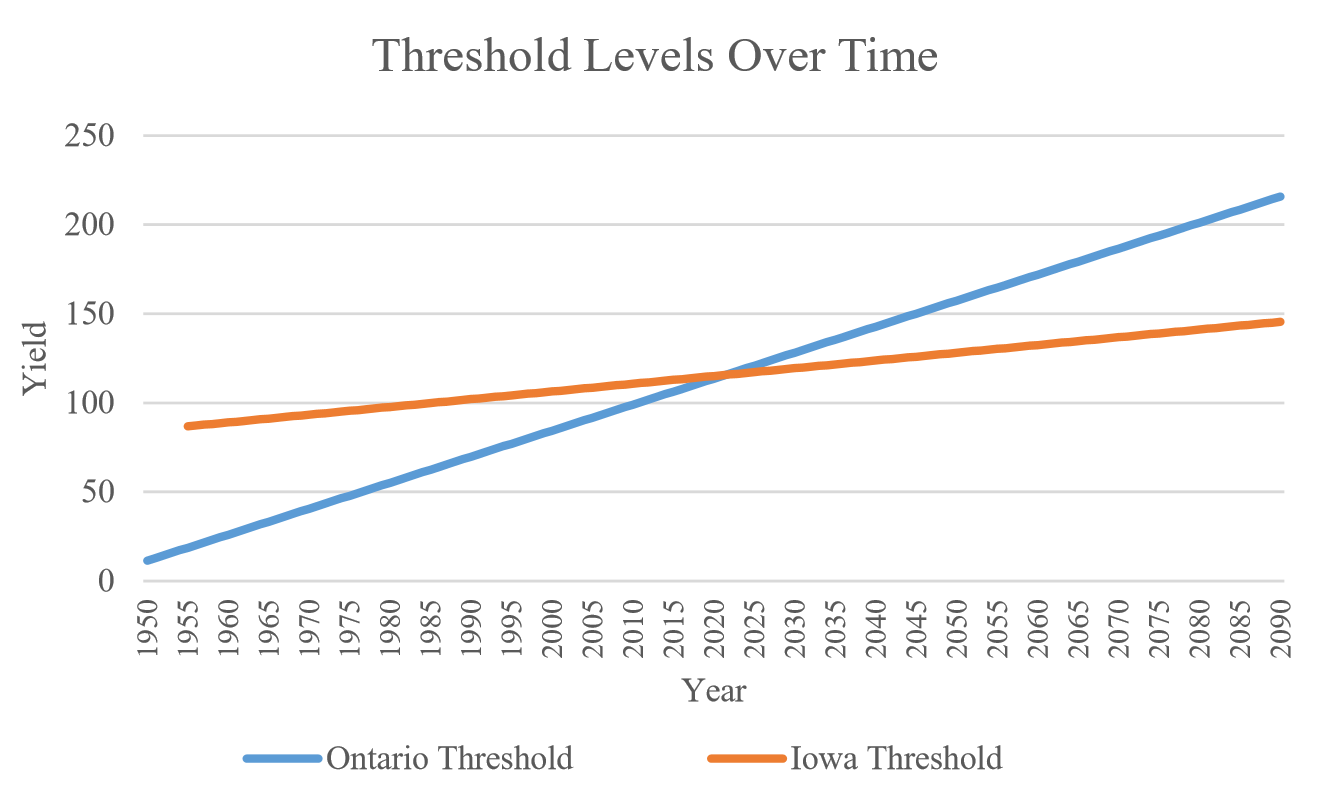
\includegraphics[width=\textwidth]{thresholdlevelstime.png}
    \caption{Threshold Levels Over Time}
 \end{figure}

The results suggest that given the more quickly increasing precipitation threshold, Ontario will be more sensitive to management practices which increase the soil water holding capacity, such as soil rotations, and practices which increase the level of soil organic matter \citep{williams2016soil}. If the increase in demand continues in the future, these sensitivities could become increasingly apparent.

The expected yields under climate change behaved differently in Iowa and Ontario. In both locations, climate change appeared to lead to increased yield variability due to weather. However, in Ontario the mean expected yields increased under climate change while they slightly decreased in Iowa. This is likely attributable to the relative current temperatures in these locations. Iowa is relatively warm in comparison to Ontario. Currently, Iowa tends to receive high $GDD$ accumulation levels over the corn growing season, and is subject to a more significant extreme heat effect. Under climate change, both $HDD$ and $GDD$ increase. Since $HDD$ is already relatively high under current climate the $HDD$ in Iowa increases more than in Ontario and the relative negative temperature effect is greater. Additionally, since $GDD$ does not increase when temperatures are above 29 degrees Celsius, which occurs more commonly in Iowa, the increased temperature under climate change increases the $GDD$ measure more in Ontario than in Iowa. Therefore, the positive heat effect is more substantial in Ontario. This explains why the effect of climate change may be different in the two study locations. The observation of this effect suggests that Ontario, and other relatively northern areas of agricultural production, could be relatively more competitive under climate change.

\section{Further Research}

Consideration of a wider variety of potential climate change scenarios given the dynamic precipitation yield model should be considered. The effect of climate change was considered in only one potential case. Generating yields given a wider variety of scenarios could give a better idea of the potential range of climate change effects on corn yields. Considering how premium rates could develop under these various scenarios would also be of interest.

The large increase in yield per acre over the study period is not unique to corn. Additionally, corn is not the only crop which is primarily rain fed. This problem could therefore apply to other crops in other locations. Additionally, the precipitation effect during the pollination and silking growth stage was the focus of this paper. It is possible that changes in the precipitation effect during other growth stages could also empirically be demonstrated over time. 

Given that the results show that the precipitation demand is increasing over time, the economic viability of irrigation systems could also be changing. Further research could attempt to estimate the profitability of irrigation systems given different climate scenarios. In this way, an estimate of when and where irrigation could become a profitable production choice could be estimated. Additionally, the value of farm management practices which can increase the soil water holding capacity could be considered.

Another point of interest is how specific corn varieties differ in terms of their responses to these types of constraints. Further research could consider what types of corn varieties are the least sensitive to drought conditions as well as to extreme heat. Estimates of the relative cost to the public of insuring these different varieties under various climate scenarios could be computed. 

\section{Policy Recommendations}


The results suggest that precipitation induced yield variability will likely increase, given that precipitation demand appears to be increasing over time, and given that precipitation could become more variable under climate change. If yields become more variable, crop insurance payouts will become more common. This implies that premium rates will likely need to increase in the future. Since the cost is shared with the public, this means that the cost of crop insurance programs may increase. Crop insurance in generally subsidized in order to attempt to increase program participation. However, it has been suggested that due to the lower share of risk held by the producer, subsidized crop insurance could increase the likelihood that the producer will make risky production decisions \citep{kerRMP2016}. Estimating the correlation between subsidy levels and overall yield variability over time could quantify this. Given that climate change may increase yield variability, other methods which can counteract this affect may become important. The potential for the lowering of yield variance over time through decreasing subsidy levels should be considered. 


The results of this thesis show that excessive heat and low precipitation decreases mean yields and increases yield variability, in agreement with \cite{williams2016soil} . 	\cite{lee2015topsoil} found that when precipitation was high, stability was increased in that the yields were not as sensitive to shallow top soil. This suggests that measures to increase soil moisture, such as irrigation, would more likely be beneficial in areas with thinner top soil depths. Conservation practices can decrease the sensitivity of crops to water by increasing the amount of water that can be held in the soil and therefore making it less likely that water will limit yield potentials \citep{IowaSWCS}. Tillage increases the evaporation rate of water from soil and may therefore be detrimental to yields, especially if precipitation becomes more variable or in areas where soils do not retain water well \citep{IowaSWCS}. Deeper soil allows the corn plant to root more deeply, and can decrease it's sensitivity to rain patterns \citep{Guilpart}. Top soil erosion negatively impacts corn yield through the inability to absorb rainfall quickly. This can lead to a higher rate of run off and therefore a decrease in the total amount of water available to the plant \citep{Guilpart}. This suggests policy decisions which encourage producers to maintain soil quality and to increase the level of soil organic carbon content so that they can hold a larger capacity of water and thereby decrease the lilkelihood that precipitation levels will limit yield.  Management practices which support this outcome include no till or reduced till farming, and using compost or cover crops to increase the organic material however the soil type in the region limits the effectiveness of these practices \citep{williams2016soil}.

\section{Main Results and Research Contributions}

The first question to be answered in this thesis was whether the relationship between corn yield and precipitation has changed over time. The results suggest that the level of precipitation required to attain high yields has increased over time in both Iowa and Ontario as expected. Under current climate, the estimated actuarially fair premium rates estimated using the static model were biased down, under the assumption that the dynamic model is correct. Given the future simulated climate, the estimated actuarially fair rates in Iowa were higher when the static model was assumed while in Ontario the resulting premium rates were not significantly different. Finally, based on model averages assuming the A1B climate scenario of the IPCC, the effect of potential climate change on yield relative to current climate and technology levels was considered. In Iowa the yield realizations were slightly higher on average and had slightly lower variance on in the current climate assumption. In Ontario however the average yield appeared to increase under climate change as did the variance. These differences in results are likely due to the difference in current climate between Iowa and Ontario. Based on this research, it appears that an awareness of the changing yield precipitation relationship can have implications for predicting losses for a crop insurer. The demand for precipitation appears to be increasing through time as stated above. If this trend were to continue it could result in an increase in the probability that precipitation will be a limiting factor for yields. This possibility could alter the profitability of irrigation systems and other agricultural technologies, such as drought resistant corn plants. 

This thesis contributes to the literature on corn yield modelling and crop insurance through the consideration of a dynamic relationship between weather variables and corn yield. The use of threshold levels to allow a non linear precipitation-yield effect was not encountered in the literature. Furthermore, the use threshold levels to empirically test whether the yield-precipitation relationship was changing through time was novel. These modifications to the commonly used linear model increase flexibility and suggest the existence of trends which were not previously considered empirically. The differences in the resultant premium estimates when assuming a static versus a dynamic yield precipitation relationship demonstrate the potential practical ramifications of the main result. Finally, the consideration of potential climate effects on expected yields suggested that the effect of climate change on agriculture will likely depend on the underlying distribution of key weather variables under current climate. It appears that climate change will likely increase yield variability in the locations studied. However, mean yields could be expected to increase in the relatively cold Ontario region, while they may decrease in Iowa. This suggests that climate change will likely alter the locations which have comparative agricultural advantage. When temperatures increase, new regions which were previously too cold to be fit for agriculture may become available for use in agricultural production. Therefore, climate change could lead to differences in where agricultural commodities are produced. This thesis empirically tested whether the precipitation-yield relationship had changed through time and concluded that it had. This changing relationship was found to have significant effects on the estimation of the actuarially fair level of crop insurance premium rates. Finally, the climate change scenario simulated suggested that yield variability would increase in both Ontario and Iowa under climate change.




















\bibliographystyle{plainnat}
\bibliography{mybib}

\chapter{Appendix}
\section{Creating Weather Variables from Raw Data}

The weather variables used in the yield model estimation were created using raw data containing daily county level precipitation, vapor pressure deficit and maximum and minimum temperatures. The code used to create these variables for Iowa is shown, the equivalent procedure was completed in Ontario.

\subsection{Iowa - code used to create weather variables for yield model}

\begin{lstlisting}

setwd("C:/Users/Regan/Google Drive/Thesis Presentations and Proposal/Thesis")

N <- 99
T <- 58

iowa <- readRDS("Data needed to complete empirical work/Daily weather data/Iowa/weather_raw_daily.rds")
df <- iowa[order(iowa$county),]
df <- df[order(df$year),]

df <- df[df$days %in% c(1:65,67:366),]

attach(df)

hdd <- NULL
tot <- NULL
UPP <- 29
LOW <- 10

for (i in 1:nrow(df))
  {
  ifelse(i/20000==floor(i/20000),print(i),0)
  
  M <- (max[i]+min[i])/2
  W <- (max[i]-min[i])/2

  psi <- ifelse(max[i]>UPP,ifelse(min[i]<UPP,asin((UPP-M)/W),(-pi/2)),0)

  hdd[i] <- ifelse(max[i]>UPP,ifelse(min[i]<UPP,((M-UPP)*((pi/2)-psi)+W*cos(psi))/pi,M-UPP),0 )

  theta <- ifelse(max[i]>LOW,ifelse(min[i]<LOW,asin((LOW-M)/W),(-pi/2)),0)

  tot[i] <- ifelse(max[i]>LOW,ifelse(min[i]<LOW,((M-LOW)*((pi/2)-theta)+W*cos(theta))/pi,M-LOW),0)
}

gdd <- tot-hdd

fdd <- NULL
FREEZE <- -2
tot_cold <- NULL
COLD <- 2

for(i in 1:nrow(df))
{ifelse(i/20000==floor(i/20000),print(i),0)
  M <- (max[i]+min[i])/2
  W <- (max[i]-min[i])/2

  psi <- ifelse(min[i]<FREEZE,ifelse(max[i]>FREEZE,asin((FREEZE-M)/W),pi/2),0)
  
  fdd[i] <- ifelse(min[i]<FREEZE,ifelse(max[i]>FREEZE,((FREEZE-M)*(psi+(pi/2))+W*cos(psi))/pi,FREEZE-M),0)
  
  theta <- ifelse(min[i]<COLD,ifelse(max[i]>COLD,asin((COLD-M)/W),pi/2),0)
  
  tot_cold[i] <- ifelse(min[i]<COLD,ifelse(max[i]>COLD,((COLD-M)*(theta+pi/2)+W*cos(theta))/pi,COLD-M),0)}


cdd <- tot_cold-fdd

#calculating the gdd according to the agronomic formula in farenheit

max_farenheit <- (max*(9/5))+32
min_farenheit <- (min*(9/5))+32

max_gdd_ag <- (max_farenheit*as.numeric(max_farenheit<86))+(86*(max_farenheit>86))
max_gdd_ag <- (max_gdd_ag*as.numeric(max_gdd_ag>50))+(50*(max_gdd_ag<50))

min_gdd_ag <- (min_farenheit*as.numeric(min_farenheit>50))+(50*(min_farenheit<50))
min_gdd_ag <- (min_gdd_ag*as.numeric(min_gdd_ag<86))+(86*(min_gdd_ag>86))

gdd_ag <- ((max_gdd_ag+min_gdd_ag)/2-50)


#calculating the CHU according to method of OMAFRA

Ymax <- 3.33*(max-10)-0.084*((max-10)^2)
Ymax <- Ymax*(Ymax>0)

Ymin <- 1.8*(min-4.4)
Ymin <- Ymin*(Ymin>0)


CHU <- (Ymax+Ymin)/2

daily_weather_iowa <- data.frame(year,county,days,min,max,gdd,hdd,cdd,fdd,gdd_ag,pcp,vpd,CHU)

saveRDS(daily_weather_iowa,file="Data needed to complete empirical work/Daily weather data/Iowa/daily_weather_iowa")


\end{lstlisting}


\section{Estimating Planting Date}

\subsection{Iowa}

The planting date model was estimated using the calibrated planting date data for Iowa. This model was then used to create estimated planting dates for the years not included in the data set. The code for both the estimation of the planting model based on the calibrated planting data and its use to create estimated planting dates for all years included in the study is shown below. The results of the model estimation can be found in table 3.1 in the Methods section.

\subsubsection{Code for Creation of Planting Date Model and Planting Date Estimate in Iowa}



\begin{lstlisting}

setwd("C:/Users/Regan/Google Drive/Thesis Presentations and Proposal/Thesis")

weather <- readRDS("Data needed to complete empirical work/Daily weather data/Iowa/daily_weather_Iowa")

planting <- read.delim(file="Data needed to complete empirical work/Planting Date data/Iowa/county_planting_dates_iowa.txt",header=T,sep="\t")
silking <- read.delim(file="Data needed to complete empirical work/Planting Date data/Iowa/county_silking_dates_iowa.txt",header=T,sep="\t")

predict <- unique(planting\$year)
weather_predict <-  weather[weather\$year \%in\% predict,]

adjust <-seq(0,nrow(weather_predict)-365,365)

planting_row <- planting[,3]+adjust
silking_row <- silking[,3]+adjust

planting_day <- planting[,3]
silking_day <- silking[,3]

gdd_ag_accum <- NULL
for (i in 1:length(planting_row))
{gdd_ag_accum[i]<-sum(weather_predict$gdd_ag[planting_row[i]:silking_row[i]])}

median_gdd_accum <- summary(gdd_ag_accum)[3]

#####Modelling Planting Dates#####

###based on weather in the month of April###

April1 <- seq(91,nrow(weather_predict),365)
April30 <- seq(120,nrow(weather_predict),365)

mean_temp_daily <- (weather_predict$min+weather_predict$max)/2

mean_temp_April <- NULL
for(i in 1:length(April1))
{mean_temp_April[i]<-mean(mean_temp_daily[April1[i]:April30[i]])}

pcp_April <- NULL
for(i in 1:length(April1))
{pcp_April[i]<-mean(weather_predict$pcp[April1[i]:April30[i]])}

vpd_April <- NULL
for(i in 1:length(April1))
{vpd_April[i]<-mean(weather_predict$vpd[April1[i]:April30[i]])}

#we will add in the trend as it would be if all years were included#
#1974 - 20, 1986 - 32, 1988 - 34, 1991 - 37, 1993 - 39, 2012 - 58)

trend <- c(20:32,34:37,39:58)
Time <- matrix(0,99,length(trend))
for (i in 1:length(trend))
{Time[,i] <- rep(trend[i],99)}
trend <- as.vector(Time)

mod <- lm(planting_day ~ mean_temp_April+vpd_April+pcp_April+trend)

Beta_planting <- summary(mod)$coeff[,1]

#formatting table for latex using stargazer package#

install.packages("stargazer")
library(stargazer)
stargazer(mod, title="Planting Date Model Results", align=TRUE)

#####Creating the estimated planting dates from our model#####

###Creating the April weather data for all years in study###

April1 <- seq(91,nrow(weather),365)
April30 <- seq(120,nrow(weather),365)

mean_temp_daily <- (weather$min+weather$max)/2

mean_temp_April <- NULL
for(i in 1:length(April1))
{mean_temp_April[i]<-mean(mean_temp_daily[April1[i]:April30[i]])}

pcp_April <- NULL
for(i in 1:length(April1))
{pcp_April[i]<-mean(weather$pcp[April1[i]:April30[i]])}

vpd_April <- NULL
for(i in 1:length(April1))
{vpd_April[i]<-mean(weather$vpd[April1[i]:April30[i]])}

trend <- c(1:58)
Time <- matrix(0,99,length(trend))
for(i in 1:length(trend))
{Time[,i] <- rep(trend[i],99)}
trend <- as.vector(Time)

const <- rep(1,length(trend))

X <- cbind(const,mean_temp_April,vpd_April,pcp_April,trend)

planting_day_estimate <- X%*%Beta_planting

adjust <- seq(0,nrow(weather)-365,365)

planting_row_estimate <- planting_day_estimate+adjust

county <- rep(unique(weather$county),58)

year <- c(1955:2012)
Year <- matrix(0,99,length(year))
for(i in 1:length(year))
{Year[,i]<-rep(year[i],99)}
year <- as.vector(Year)

planting_day_estimate <- data.frame(cbind(year,county,planting_day_estimate))

###creating the estimated silking dates based on the planting dates###

#the silking dates will be the point at which the median gdd_ag accumulation occurs after planting date#

silking_row_estimate <- NULL

Aug30 <- seq(242,nrow(weather),365)
for(i in 1:length(planting_row_estimate))
{accum_gdd_ag <- 0
for(j in planting_row_estimate[i]:Aug30[i])
{accum_gdd_ag<- weather$gdd_ag[j]+accum_gdd_ag
if(accum_gdd_ag>=median_gdd_accum)
{silking_row_estimate[i] <- j
break}}
}

silking_day_estimate <- silking_row_estimate-adjust

silking_row_estimate <- data.frame(year,county,silking_row_estimate)
silking_day_estimate <- data.frame(year,county,silking_day_estimate)

#testing the level of error in the silking date estimates using known values

silk_test <- silking_day_estimate[silking_day_estimate$year %in% predict,]

silk_predict <- silk_test[,3]

mod <- lm(silking_day ~ 0+silk_predict)

#Residual standard error of 5.412 when using the predicted planting days to guess the known silking days#

###now we want to replace the known years with the values we have instead of keeping them as the predicted values###

new <- planting_day_estimate[planting_day_estimate$year %in% predict,]

rownumberknown <- row.names(new)

for (i in 1:length(rownumberknown))
{planting_day_estimate[rownumberknown[i],] <- planting[i,]}

for(i in 1:length(rownumberknown))
{silking_day_estimate[rownumberknown[i],] <- silking[i,]}

adjust <- seq(0,nrow(weather)-365,365)
planting_row_estimate <- planting_day_estimate[,3]+adjust
planting_row_estimate <- data.frame(year,county,planting_row_estimate)

silking_row_estimate <- silking_day_estimate[,3]+adjust
silking_row_estimate <- data.frame(year,county,silking_row_estimate)

saveRDS(planting_row_estimate,"Data needed to complete empirical work/Planting Date data/Iowa/planting_row_estimate")
saveRDS(silking_row_estimate,"Data needed to complete empirical work/Planting Date data/Iowa/silking_row_estimate")

\end{lstlisting}


\subsection{Ontario}

\subsubsection{Code for Creation of Planting Date Estimate in Ontario}

In Ontario there was no available planting date data which could be accessed. The method which has commonly been used by OMAFRA of taking the planting date to be the first day in the spring after which 3 days in a row have average temperatures of more than 12.8 degrees Celcius was used. \citep{OMAFRAhybrid}.

\begin{lstlisting}

setwd("C:/Users/Regan/Google Drive/Thesis Presentations and Proposal/Thesis")

weather <- readRDS("Data needed to complete empirical work/Daily weather data/Ontario/daily_weather_ontario")

counties <- c("brant","bruce","chatham-kent","dufferin","elgin","essex","grey","haldimand-norfolk",
		"halton","hamilton","hastings","huron","kawartha lakes","lambton","lanark",
		"leeds-grenville","lennox-addington","middlesex","niagara","northumberland",
		"ottawa","oxford","peel","perth","prescott-russell","prince edward","renfrew",
		"simcoe","stormont-dundas-glengarry","waterloo","wellington","york")


weather <- weather[weather$county %in% counties,]

attach(weather)

#calculating planting date as the day after 3 consecutive days with temp over 12.8 degrees celcius

April1 <-  seq(91,nrow(weather),365)
June1 <- seq(152,nrow(weather),365)
plant <- NULL
for(i in 1:length(April1))
{for(j in April1[i]:June1[i])
{if(((weather$max[j]+weather$min[j])/2)>=12.8 && ((weather$max[j+1]+weather$min[j+1])/2)>=12.8  && ((weather$max[j+2]+weather$min[j+2])/2)>=12.8)
{plant[i]<- (j+3)
break}
else{plant[i] <- (June1[i]+3)}}}

silk <- NULL

accum_gdd_ag <- 0
Aug30 <- seq(242,nrow(weather),365)
for(i in 1:length(plant))
{accum_gdd_ag <- 0
for(j in plant[i]:Aug30[i])
{accum_gdd_ag<- weather$gdd_ag[j]+accum_gdd_ag
if(accum_gdd_ag>=1400)
{silk[i] <- j
break}
else{silk[i] <- Aug30[i]}}}

year <- unique(year)
Year <- matrix(0,length(unique(county)),length(year))
for (i in 1:length(year))
{Year[,i]<-rep(year[i],length(unique(county)))}
year <- as.vector(Year)

county <- rep(unique(county),length(unique(year)))

planting_row_estimate <- plant
planting_row_estimate <- data.frame(year,county,planting_row_estimate)

silking_row_estimate <- silk
silking_row_estimate <- data.frame(year,county,silking_row_estimate)

saveRDS(planting_row_estimate,"Data needed to complete empirical work/Planting Date data/Ontario/planting_row_estimate")
saveRDS(silking_row_estimate,"Data needed to complete empirical work/Planting Date data/Ontario/silking_row_estimate")

\end{lstlisting}

\section{Model Testing}

As was discussed in the methods section various models with different combinations of variables and different ways of timing those variables were tested. To do this unique data sets which included variables corresponding to those required for each model were created. Each model was estimated using the corresponding created data set according to the procedure described in the methods section and the results were stored. Finally the most appropriate model was chosen based on the degree of model fit and the coefficient values. Below the various ways in which the variables were timed and the agronomic reasons for these timings are discussed.

\subsection{Agronomic Growth Stages and Growing Degree Days for Corn}

Growth stage dates are approximated by accumulated heat units beginning at the date of planting. Growing degree days (GDD) were used as the measure of accumulated heat units. Planting and silking data for the years that it was available in Iowa was used to test whether the agronomic estimates of the number of growing degree days which are accumulated from the planting date to the start of the silking date was accurate. Generally silking starts approximately when 1400 GDD have been accumulated since the planting date \citep{neild1987growing}. The median number of growing degree days which had accumulated between the calibrated planting and silking dates was 1389 and the mean was 1394, very similar to the 1400 generally assumed in theory. GDD accumulation from planting date estimates were used to time growth stages with silking stage assumed to start after 1389 GDD had accumulated. The table below shows the approximate growing degree day accumulations associated with the beginning of various corn growth stages.

\begin{table}[!htbp]
\caption{Corn Development and Growing Degree Days \citep{neild1987growing}}
\label{GDD_tab}
\begin{tabular}{lll}
\hline
Phase        & Development Stage                                                                                & GDD  \\
\hline
Vegetative   &                                                                                                  &      \\

             & Planted                                                                                          & 0    \\
             & Two leaves fully emerged                                                                         & 200  \\
             & Four eaves fully emerged                                                                         & 345  \\
             & Six leaves fully emerged (Growing point above soil) & 475  \\
             & Eight leaves fully emerged (Tassel beginning to develop)                                         & 610  \\
             & Ten leaves fully emerged                                                                         & 740  \\
             & Twelve leaves fully emerged (Ear formation)                                                      & 870  \\
             & Fourteen leaves fully emerged (Silks developing on ear)                                          & 1000 \\
             & Sixteen leaves fully emerged (Tip of tassel emerging)                                            & 1135 \\

Reproductive &                                                                                                  &      \\

             & Silks emerging/pollen shedding (Plant at full height)                                            & 1400 \\
             & Kernels in blister stage        & 1660 \\
             & Kernels in dough stage                                                                           & 1925 \\
             & Kernels denting                                                                                  & 2190 \\
Maturation   &                                                                                                  &      \\

             & Kernels dented                                                                                   & 2450 \\
             & Physiological maturity                                                                           & 2700\\
\hline
\end{tabular}
\end{table}


As the corn plant moves through these stages its input requirements change. As the number of leaves increase the plant is at an increased risk of damage from high temperatures and low precipitation levels \citep{neild1987growing}. As the tassel begins to emerge this sensitivity increases due to the possibility that pollen can be denatured from extreme heat or lack of water \citep{OMAFRA}. The silks emerge soon after this and are receptive to pollen. Environmental stress is very detrimental to yield at this point and stress due to lack of moisture in particular can damage the silks \citep{OMAFRA}. After pollination the grain filling period begins \citep{neild1987growing}. Precipitation after grain filling is complete is not as important for yield realization \citep{neild1987growing}. 

Detrimental effects from extreme heat reach a maximum during the silking and pollination period while cold temperature stress can be dangerous during early growth and emergence, or after pollination in the case of frost previous to denting \citep{OMAFRA}. Due to the distribution of temperature in North American climate it can be seen that extreme heat mostly occurs during the period at which it is most damaging. Cold temperatures are generally problematic at the beginning and end of the growing season which is the only time they are likely to occur. Because of this I did not alter the timing of any of the heat variables included in the various models when completing model testing and the heat variables are accumulations over the entire season. Therefore only the precipitation and vapour pressure deficit were subject to changes under different variable timing methods. Below I discuss the various timings that were considered.

\subsection{Variable Timing Profiles considered in Model Testing}

\subsubsection{Timing 0 - Mean of Variables over Growing Season}

Timing method 0 simply takes the averages of the precipitation and vapor pressure deficit variables over the entire growing season. The growing season is considered to begin at the estimated planting date and end at the estimated maturity date which is when 2700 growing degree days have accumulated after the planting date.

\subsubsection{Timing i - Accumulated Precipitation and Vapor Pressure Deficit over 3 stages of the Growing Season}

Timing i breaks up the growing season into 3 stages. The 3 stages correspond to the beginning of the season - planting to silking stage, the silking and pollination stage, and finally the end of the season - from pollination to maturity. The timing of the variables all have some days added to either side for buffering. The resulting variables are as follows:

$$\text{Precipitation for beginning of season stage: }PCP_b=sum(PCP(\text{planting:silking-5}))$$
$$\text{Precipitation for pollination stage: }PCP_pol=sum(PCP(\text{silking-4:silking+14}))$$
$$\text{Precipitation for end of season stage: }PCP_e=sum(PCP(\text{silking+15:maturity}))$$

Where $PCP$ refers to precipitation. The vapor pressure deficit variables are created in the same manner and using the same dates for timings. 

\subsubsection{Timing ii - Mean Precipitation and Vapor Pressure Deficit over 3 stages of the Growing Season}

Timing ii breaks up the stages of the growing season in the same way as timing i but takes the averages of the precipitation and vapor pressure deficit variables as opposed to their accumulated values over each period.

\subsubsection{Timing iii -  Accumulated Precipitation and Vapor Pressure Deficit for Each Month in the Growing Season}

Timing iii divides the growing season by month as opposed to by timed growth stages. The precipitation and vapor pressure deficit variables are the cumulative monthly totals from May to August when corn generally reaches maturity.

\subsubsection{Timing iv - Accumulated Precipitation and Vapor Pressure Deficit over 3 stages of the Growing Season}

Timing iv is similar to timing i in that it breaks up the growing season into 3 stages corresponding to a beginning of season stage, a pollination stage and an end of season stage. The difference with this timing is the amount of buffering applied to the variables. The timed variables are as shown below:

$$\text{Precipitation for beginning of season stage: }PCP_{b_i}=sum(PCP(\text{planting:silking-14}))$$
$$\text{Precipitation for pollination stage: }PCP_{pol_i}=sum(PCP(\text{silking-13:silking+14}))$$
$$\text{Precipitation for end of season stage: }PCP_{e_i}=sum(PCP(\text{silking+15:maturity}))$$

The vapor pressure deficit variables are created in the same manner and using the same dates for timings. 


\subsubsection{Timing v - Accumulated Precipitation and Vapor Pressure Deficit over 4 stages of the Growing Season}

Timing v splits the beginning of season precipitation variable into 2 parts. This is to consider the increasing demand for water which begins previous to the pollination and silking stage. The break point is set at the V10 stage which is marking approximately when 10 leaves have developed on the corn plant. The variables for this model are timed as shown below.

$$\text{Precipitation for beginning stage 1: }PCP_{b1_i}=sum(PCP(\text{planting:V10-10}))$$
$$\text{Precipitation for beginning stage 2: }PCP_{b1_i}=sum(PCP(\text{V10-9:silking-14}))$$
$$\text{Precipitation for pollination stage: }PCP_{pol_i}=sum(PCP(\text{silking-13:silking+14}))$$
$$\text{Precipitation for end of season stage: }PCP_{e_i}=sum(PCP(\text{silking+15:maturity}))$$

The vapor pressure deficit variables are created in the same manner and using the same dates for timings. 

\subsubsection{Timing vi - Mean of Variables over Growing Season}

Timing vi includes all of the variables in timing v but adds in an additional pre-season variable. This variable contains the accumulated pre-season precipitation and vapor pressure deficit respectively beginning in October of the previous year and ending at the time of planting. 

\subsection{Variable Groupings Considered in Model Testing}

In addition to the various methods of timing the precipitation and vapor pressure deficit variables we tested different combinations of the variables we were considering. These variables are average temperature over growing season (T), GDD, HDD, CDD, FDD, precipitation (P), and vapor pressure deficit (VPD). We tested models containing 7 different combinations of independent variables with each timing. The 7 different combinations are listed in the table below.

\begin{table}[!htbp]
\caption{Variable Grouping for Model Testing}
\label{var_groups_tab}
\begin{tabular}{l|lllllll}
\hline
                    & a & b & c & d & e & f & g \\
                    \hline
T                   & x & x &   &   &   &   &   \\
GDD                 &   &   & x & x & x & x & x \\
HDD                 &   &   &   & x & x & x & x \\
CDD                 &   &   &   &   & x &   & x \\
FDD                 &   &   &   &   &   & x & x \\
PCP                   & x & x & x & x & x & x & x \\
VPD                 &   & x & x & x & x & x & x\\
\hline
\end{tabular}
\end{table}

After the timed variables were created and grouped into data sets each timing and variable combination described was estimated as a linear model describing yields. 

\subsection{Code Used for Variable and Data set Creation for Model Testing}

The code used to create the variables and data sets for the first timing option (Timing 0) in Iowa is shown below. The generation and organization of the data for Ontario and for the other timings and combinations was very similar and is not included for the sake of space. 


\begin{lstlisting}

setwd("C:/Users/Regan/Google Drive/Thesis Presentations and Proposal/Thesis")

weather <- readRDS("Data needed to complete empirical work/Daily weather data/Iowa/daily_weather_Iowa")

#####Creating variables and data sets to test different models#####

###getting yield###

Yield <- readRDS("Data needed to complete empirical work/Yield Data/Iowa/Yield_Iowa")

yield <- Yield[,3]

year <- Yield[,1]

county <- Yield[,2]

###planting and silking date###

planting <- readRDS("Data needed to complete empirical work/Planting Date data/Iowa/planting_row_estimate")
planting <- planting[,3]

silking <- readRDS("Data needed to complete empirical work/Planting Date data/Iowa/silking_row_estimate")
silking <- silking[,3]

####0####
###a###

#mean temp and pcp over growing season#

May1 <- seq(121,nrow(weather),365)
Aug30 <- seq(242,nrow(weather),365)

mean_temp_daily <- (weather$min+weather$max)/2

mean_temp_season <- NULL
for(i in 1:length(May1))
{mean_temp_season[i] <- mean(mean_temp_daily[May1[i]:Aug30[i]])}

mean_pcp_season <- NULL
for(i in 1:length(May1))
{mean_pcp_season[i] <- mean(weather$pcp[May1[i]:Aug30[i]])}

trend <- c(1:58)
Trend <- matrix(0,99,length(trend))
for (i in 1:length(trend))
{Trend[,i] <- rep(trend[i],99)}
trend <- as.vector(Trend)


Data_a_0_iowa <- data.frame(year,county,yield,trend,mean_temp_season,mean_pcp_season)
\\
saveRDS(Data_a_0_iowa,"Data needed to complete empirical work/Data sets for model testing/Iowa/Data_a_0_iowa")

###b###

#mean temp, pcp and vpd over growing season#

mean_vpd_season <- NULL
for(i in 1:length(May1))
{mean_vpd_season[i] <- mean(weather$vpd[May1[i]:Aug30[i]])}

Data_b_0_iowa <- data.frame(year,county,yield,trend,mean_temp_season,mean_vpd_season,mean_pcp_season)
\\
saveRDS(Data_b_0_iowa,"Data needed to complete empirical work/Data sets for model testing/Iowa/Data_b_0_iowa")

###c###

#accumulated gdd mean pcp and vpd over growing season#

gdd_season <- NULL
for(i in 1:length(May1))
{gdd_season[i] <- sum(weather$gdd[May1[i]:Aug30[i]])}

Data_c_0_iowa <- data.frame(year,county,yield,trend,gdd_season,mean_vpd_season,mean_pcp_season)
\\
saveRDS(Data_c_0_iowa,"Data needed to complete empirical work/Data sets for model testing/Iowa/Data_c_0_iowa")

###d###

#gdd, hdd, mean pcp and vpd over growing season#

hdd_season <- NULL
for(i in 1:length(May1))
{hdd_season[i] <- sum(weather$hdd[May1[i]:Aug30[i]])}

Data_d_0_iowa <- data.frame(year,county,yield,trend,gdd_season,hdd_season,mean_vpd_season,mean_pcp_season)
\\
saveRDS(Data_d_0_iowa,"Data needed to complete empirical work/Data sets for model testing/Iowa/Data_d_0_iowa")

###e###

#d plus cdd#

cdd_season <- NULL
for(i in 1:length(May1))
{cdd_season[i] <- sum(weather$cdd[May1[i]:Aug30[i]])}

Data_e_0_iowa <- data.frame(year,county,yield,trend,gdd_season,hdd_season,cdd_season,mean_vpd_season,mean_pcp_season)
\\
saveRDS(Data_e_0_iowa,"Data needed to complete empirical work/Data sets for model testing/Iowa/Data_e_0_iowa")

###f###

#e with fdd subbed for cdd#

fdd_season <- NULL
for(i in 1:length(May1))
{fdd_season[i] <- sum(weather$fdd[May1[i]:Aug30[i]])}

Data_f_0_iowa <- data.frame(year,county,yield,trend,gdd_season,hdd_season,fdd_season,mean_vpd_season,mean_pcp_season)
\\
saveRDS(Data_f_0_iowa,"Data needed to complete empirical work/Data sets for model testing/Iowa/Data_f_0_iowa")

###g###

#f with cdd as well#

Data_g_0_iowa <- data.frame(year,county,yield,trend,gdd_season,hdd_season,cdd_season,fdd_season,mean_vpd_season,mean_pcp_season)
\\
saveRDS(Data_g_0_iowa,"Data needed to complete empirical work/Data sets for model testing/Iowa/Data_g_0_iowa")



\end{lstlisting}



\subsection{Results from Model Testing}

In the methods section the spatial nature of the data was discussed. The spatial correlation parameter is first estimated by maximizing the likelihood equation as described in the methods section. Then the model is reconfigured using this $\rho$ value to give $X_{new}=AX$ and $Y_{new}=AY$. The regression of $Y_{new}$ on $X_{new}$ can then be estimated by OLS. Therefore the dependent variable in the results below is $Y_{new}$ and the independent variables are the columns of $X_{new}$, however they are referred to by their variable names as they would have been in $X$. Regional dummy variables were included in each Iowa model for the 9 regions in the state and county dummy variables were included in each Ontario model for all 32 counties in the data set. In the results tables below the estimated coefficients for all of the dummy variables both in Iowa and Ontario have been removed for the sake of brevity given that they are not the variables of interest.

\subsubsection{Iowa}


 
\begin{table}[H]
    \centering
    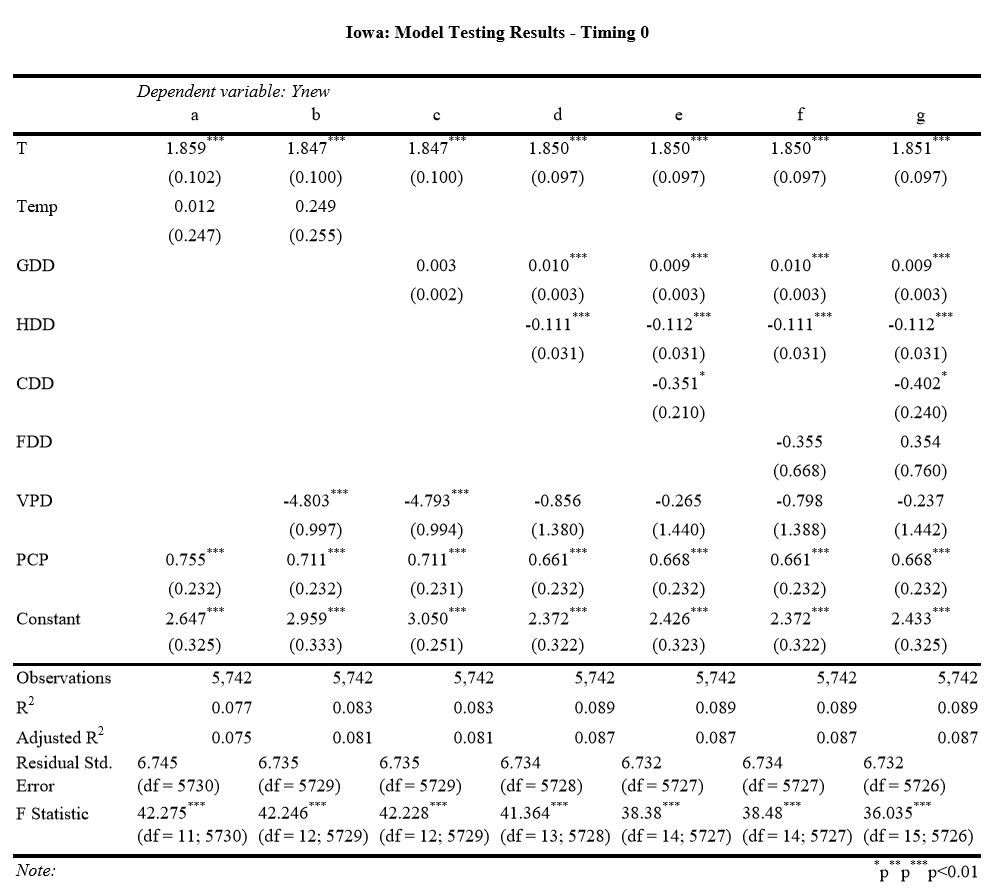
\includegraphics[width=1.0\textwidth]{IA_a_0.png}
    \caption{Iowa: Model Testing Results - Timing 0}
    \label{fig:my_label}
\end{table}

 
\begin{table}[H]
    \centering
    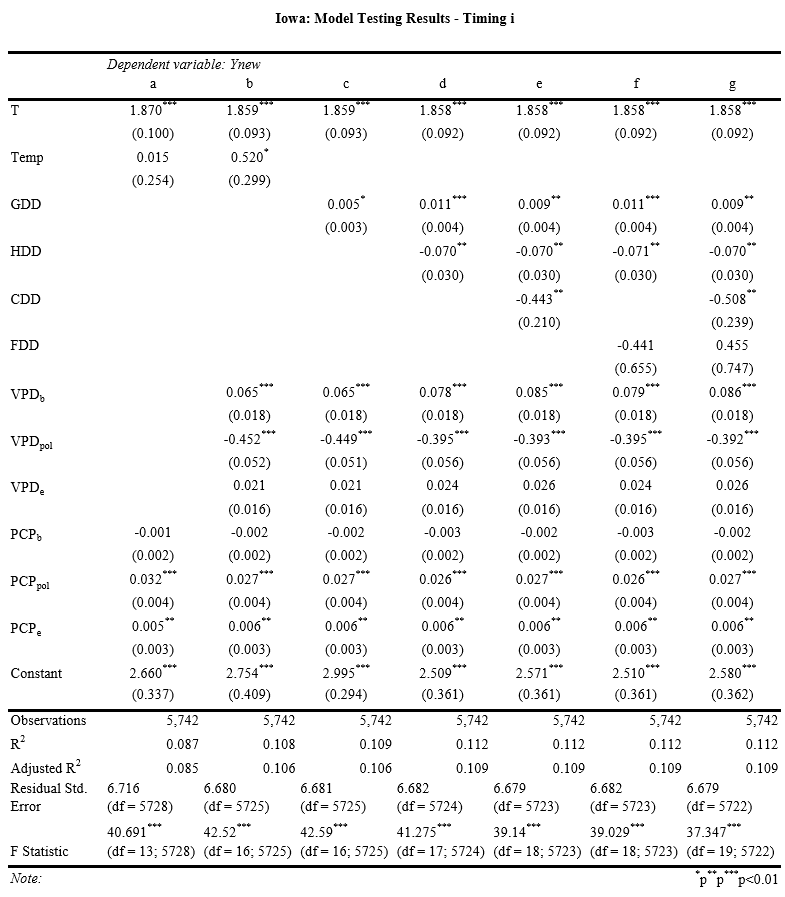
\includegraphics[width=1.0\textwidth]{IA_a_i.png}
    \caption{Iowa: Model Testing Results - Timing i}
    \label{fig:my_label}
\end{table}

 
\begin{table}[H]
    \centering
    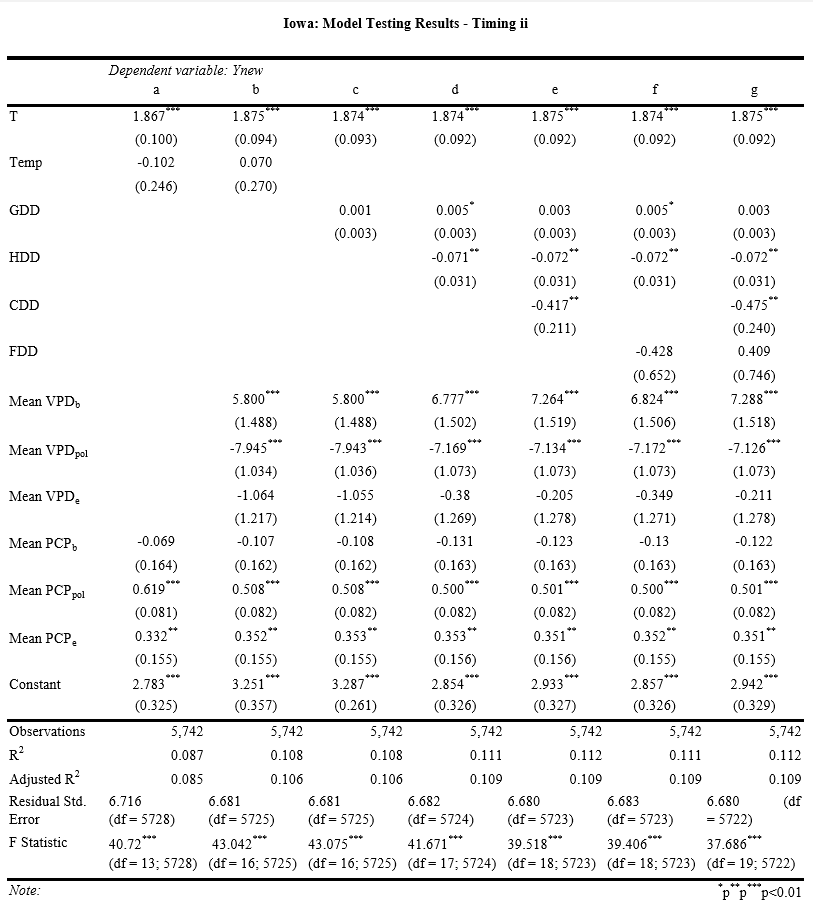
\includegraphics[width=1.0\textwidth]{IA_a_ii.png}
    \caption{Iowa: Model Testing Results - Timing ii}
    \label{fig:my_label}
\end{table}

 
\begin{table}[H]
    \centering
    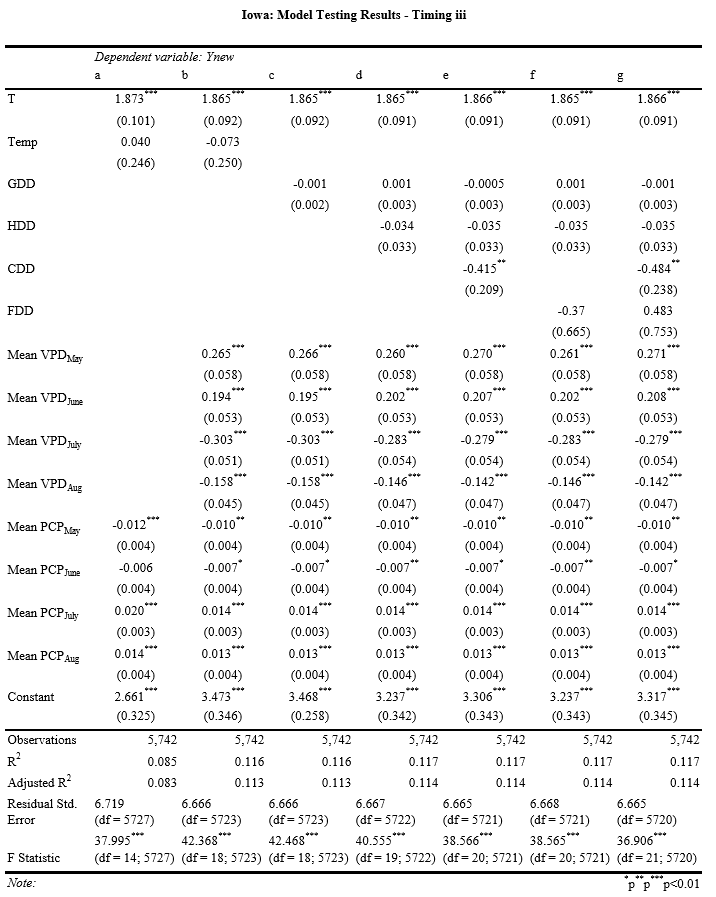
\includegraphics[width=1.0\textwidth]{IA_a_iii.png}
    \caption{Iowa: Model Testing Results - Timing iii}
    \label{fig:my_label}
\end{table}

 
\begin{table}[H]
    \centering
    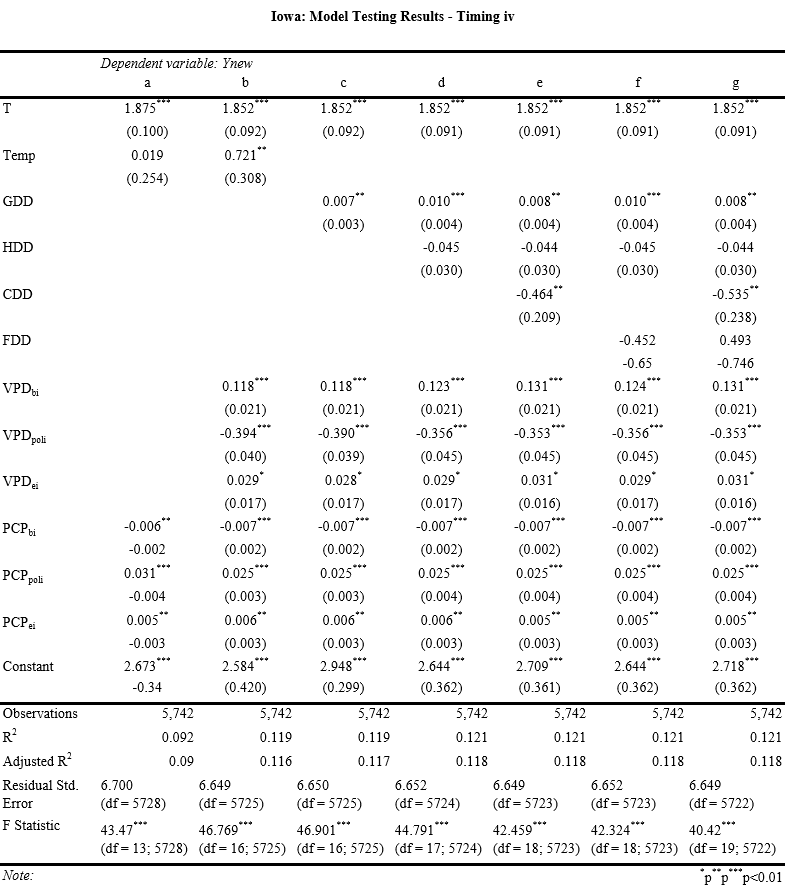
\includegraphics[width=1.0\textwidth]{IA_a_iv.png}
    \caption{Iowa: Model Testing Results - Timing iv}
    \label{fig:my_label}
\end{table}

 
\begin{table}[H]
    \centering
    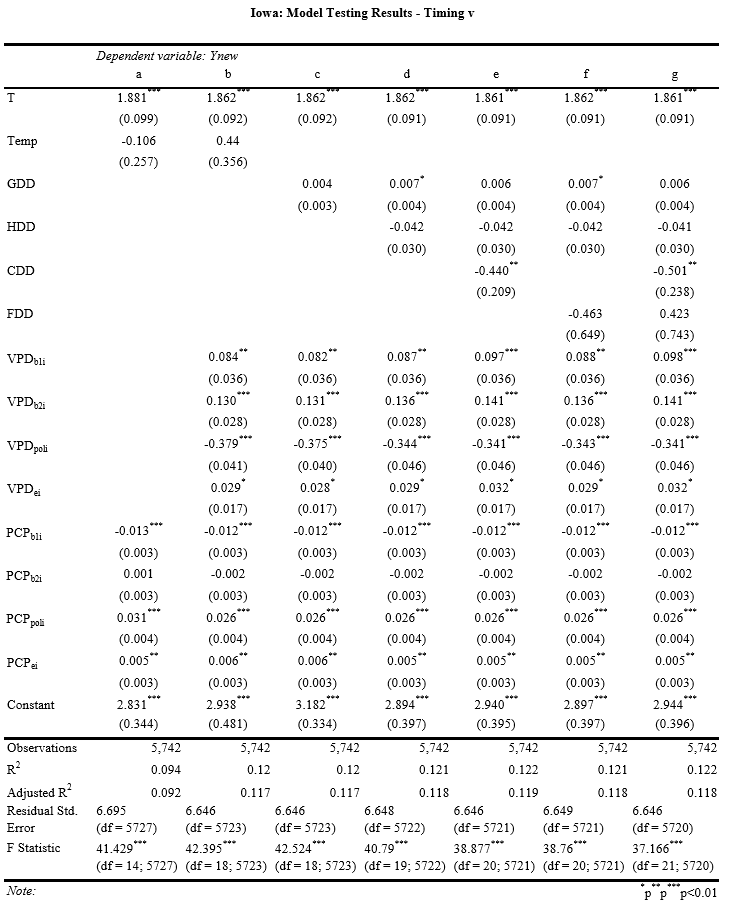
\includegraphics[width=1.0\textwidth]{IA_a_v.png}
    \caption{Iowa: Model Testing Results - Timing v}
    \label{fig:my_label}
\end{table}

 
\begin{table}[H]
    \centering
    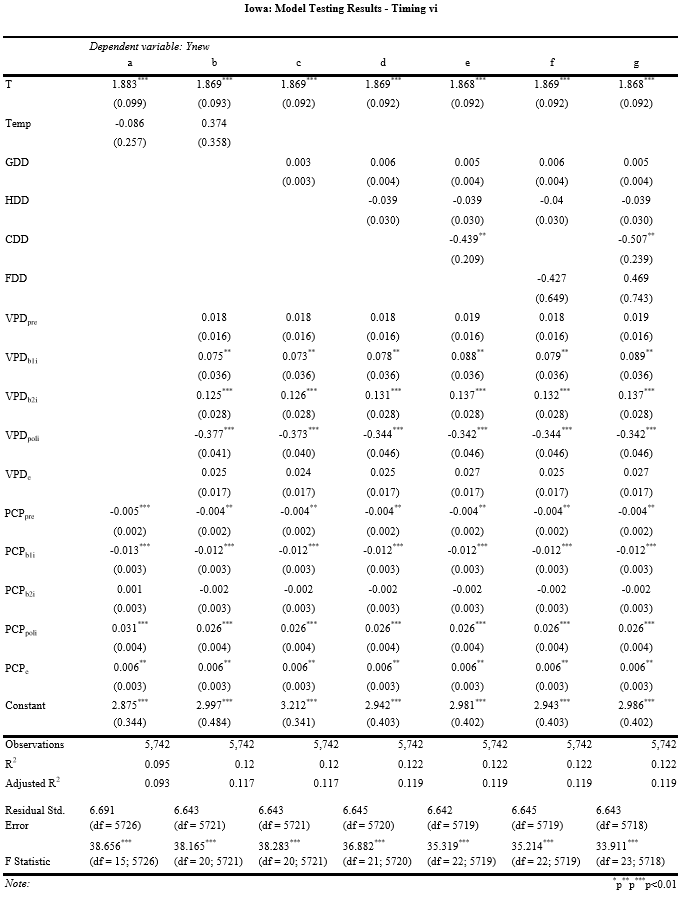
\includegraphics[width=1.0\textwidth]{IA_a_vi.png}
    \caption{Iowa: Model Testing Results - Timing vi}
    \label{fig:my_label}
\end{table}



\subsubsection{Ontario}

 
\begin{table}[H]
    \centering
    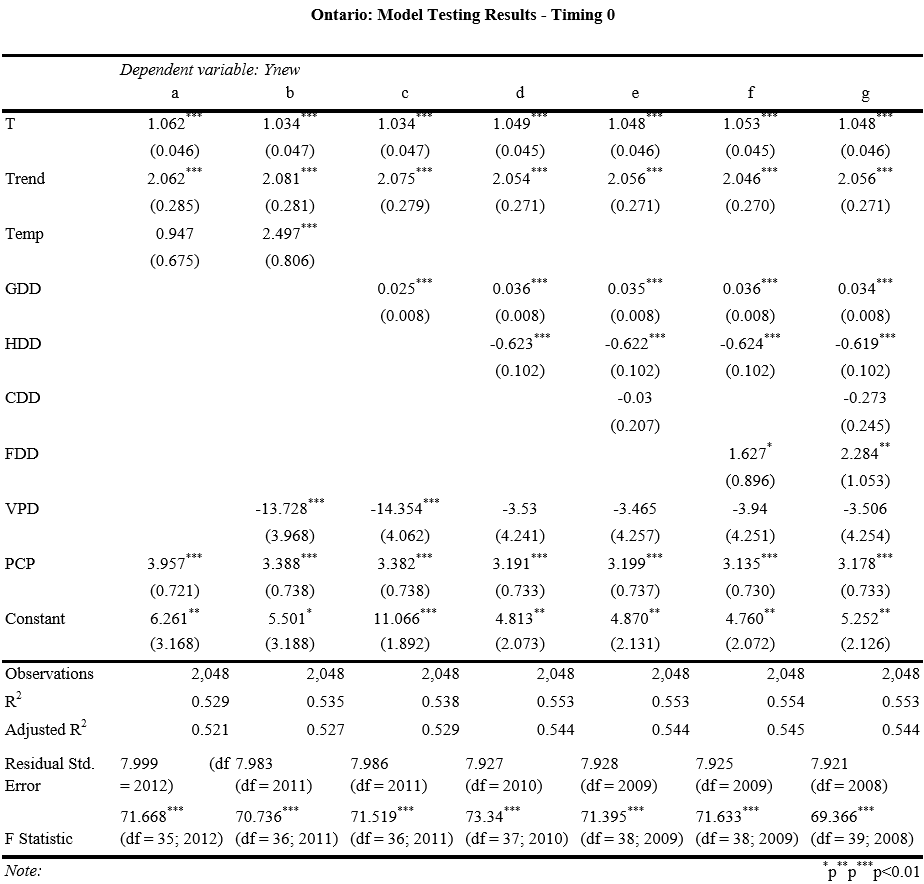
\includegraphics[width=1.0\textwidth]{ON_a_0.png}
    \caption{Ontario: Model Testing Results - Timing 0}
    \label{fig:my_label}
\end{table}

\begin{table}[H]
    \centering
    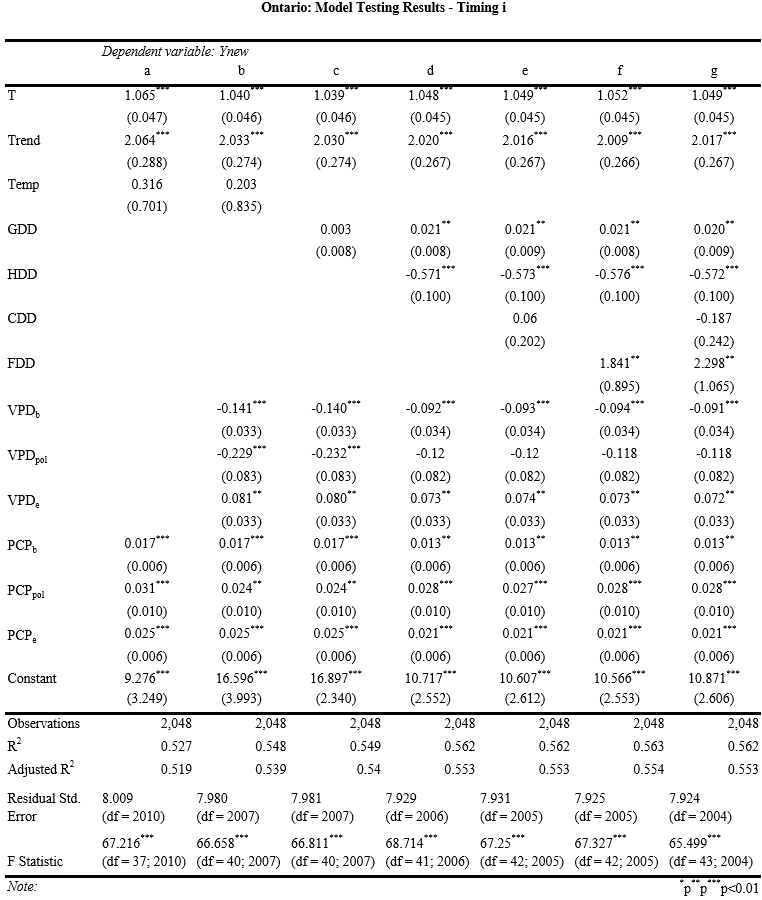
\includegraphics[width=1.0\textwidth]{ON_a_i.png}
    \caption{Ontario: Model Testing Results - Timing i}
    \label{fig:my_label}
\end{table}

\begin{table}[H]
    \centering
    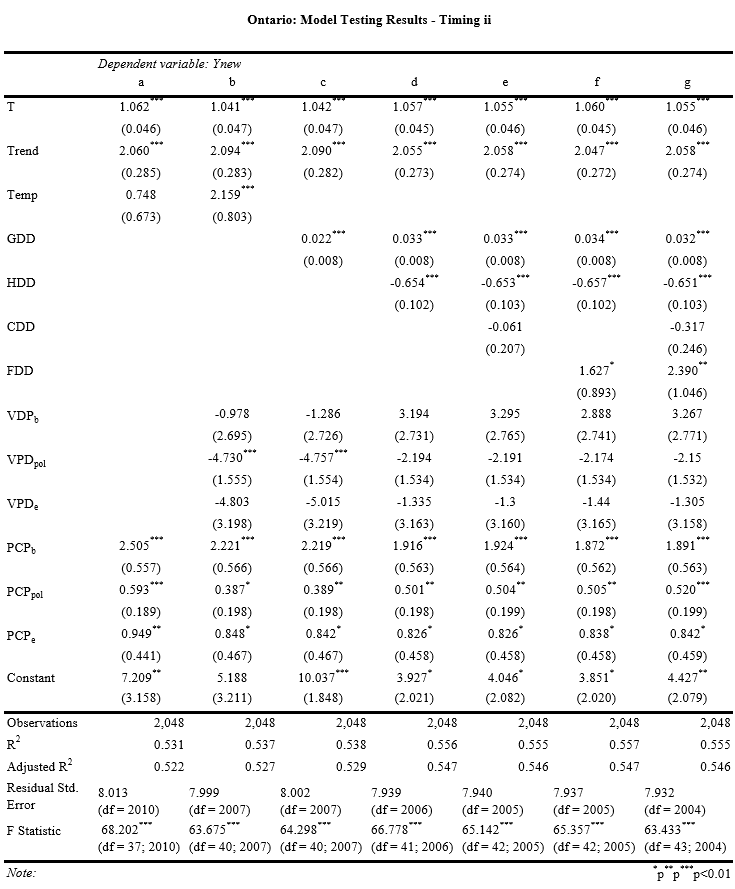
\includegraphics[width=1.0\textwidth]{ON_a_ii.png}
    \caption{Ontario: Model Testing Results - Timing ii}
    \label{fig:my_label}
\end{table}

\begin{table}[H]
    \centering
    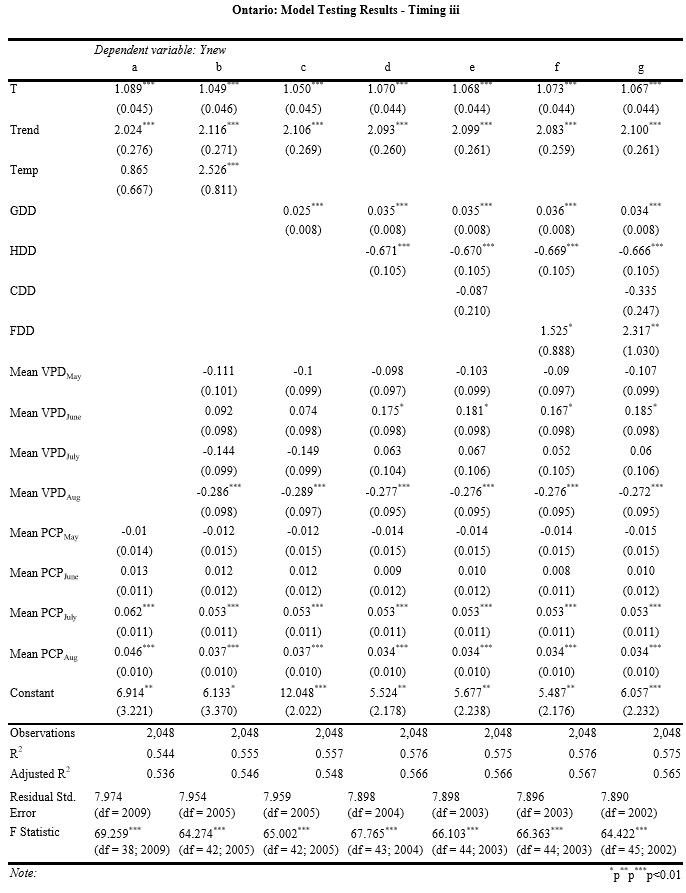
\includegraphics[width=1.0\textwidth]{ON_a_iii.png}
    \caption{Ontario: Model Testing Results - Timing iii}
    \label{fig:my_label}
\end{table}

\begin{table}[H]
    \centering
    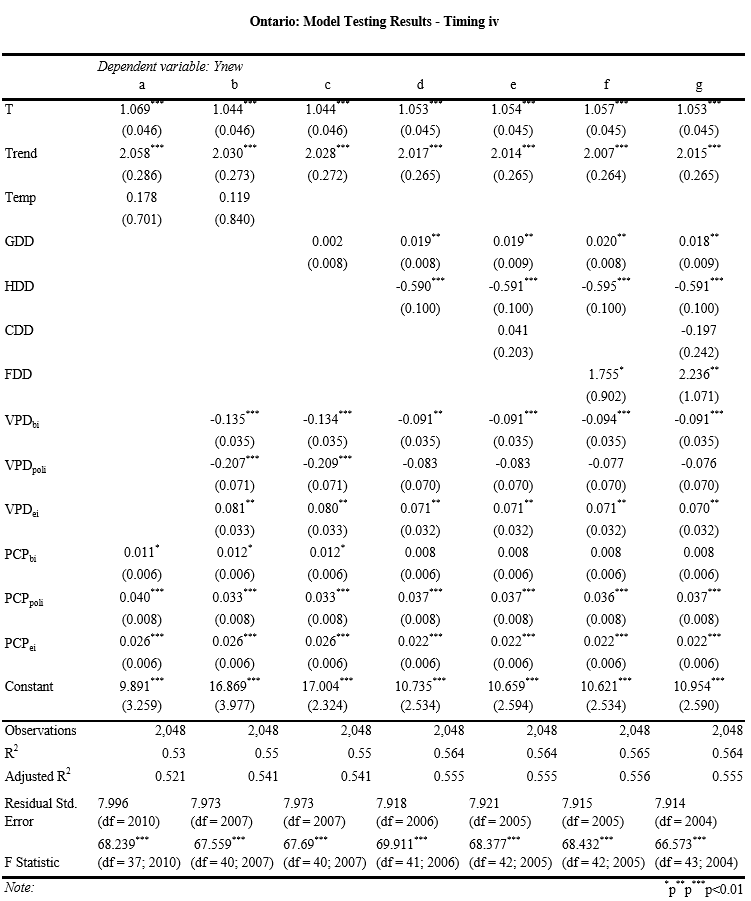
\includegraphics[width=1.0\textwidth]{ON_a_iv.png}
    \caption{Ontario: Model Testing Results - Timing iv}
    \label{fig:my_label}
\end{table}

\begin{table}[H]
    \centering
    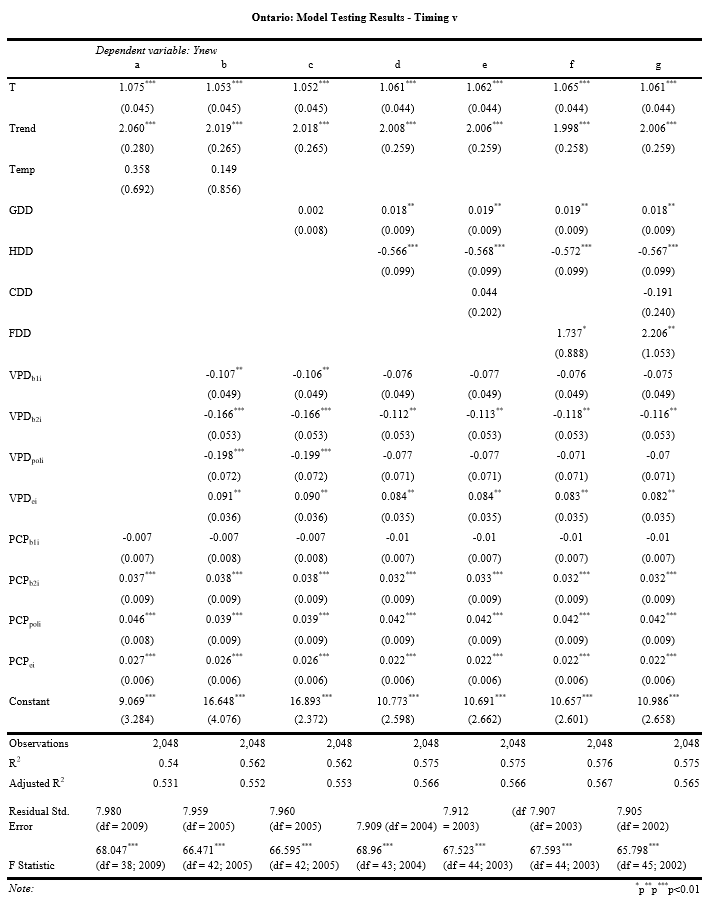
\includegraphics[width=1.0\textwidth]{ON_a_v.png}
    \caption{Ontario: Model Testing Results - Timing v}
    \label{fig:my_label}
\end{table}

\begin{table}[H]
    \centering
    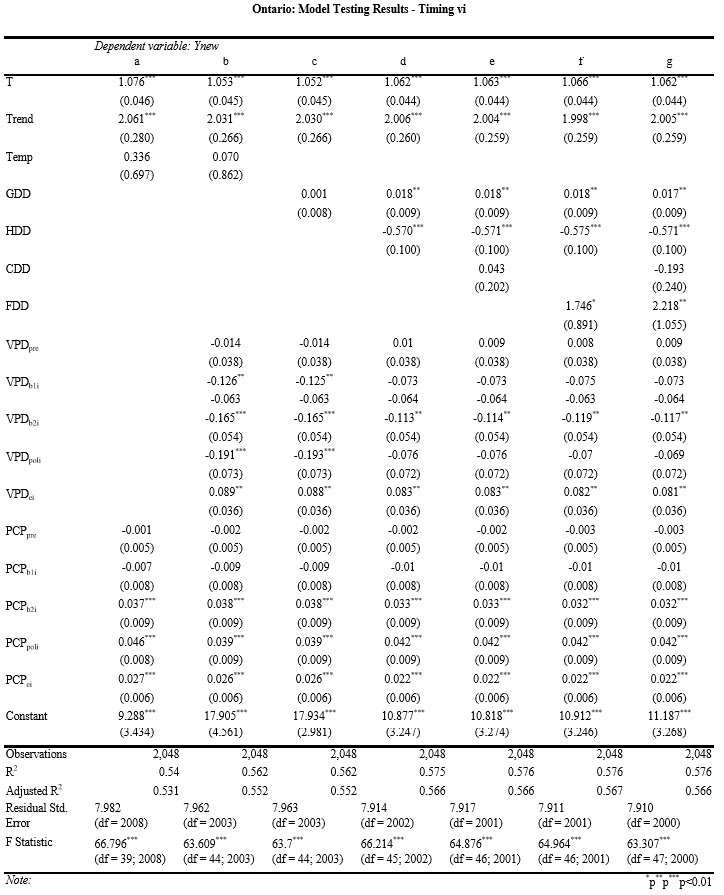
\includegraphics[width=1.0\textwidth]{ON_a_vi.png}
    \caption{Ontario: Model Testing Results - Timing vi}
    \label{fig:my_label}
\end{table}

\begin{table}[H]
   
    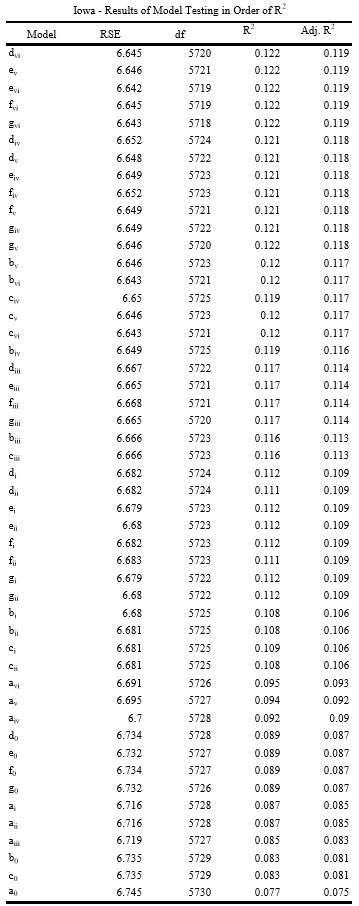
\includegraphics[width=.55\textwidth]{Iowa_r2.png}
    \caption{Iowa - Results of Model Testing in Order of R$^2$}
    \label{fig:my_label}
\end{table}

\begin{table}[H]
   
    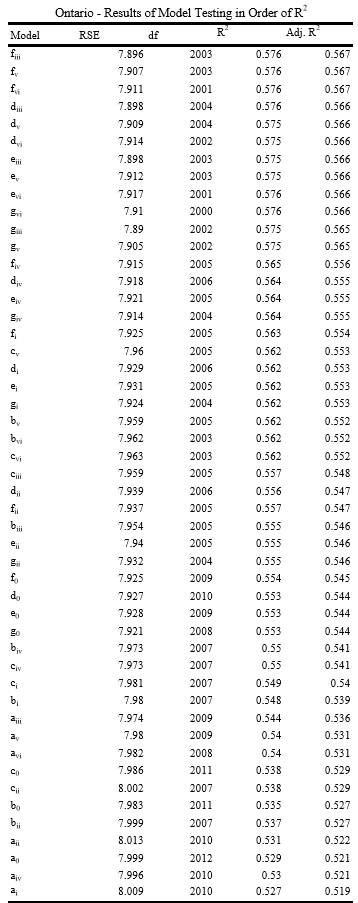
\includegraphics[width=.55\textwidth]{Ontario_r2.png}
    \caption{Ontario - Results of Model Testing in Order of R$^2$}
    \label{fig:my_label}
\end{table}


Model $div$ was chosen for Iowa. This model was selected as it was the most parsimonious model with the highest adjusted $R^2$. In Ontario the 3 models which tied for the highest adjusted $R^2$ had large positive coefficients on the FDD terms which were about 2.5 to 3 times the magnitude of the HDD coeficients from the same models. FDD represents temperatures below -2 degrees celcius which can damage corn yields when they occur both at the beginning and the end of the season \citep{OMAFRA}. These results were not logical and therefore the simpler $diii$ model was chosen for Ontario as it also had a high adjusted $R^2$.



\subsection{Code from Model Testing}

The following code was used to test each of the models considered. The data set df was set at the top and the model was evaluated given the particular combination of variables in that particular data set.

\subsubsection{Iowa}

\begin{lstlisting}


setwd("C:/Users/Regan/Google Drive/Thesis Presentations and Proposal/Thesis")

N <- 99
T <- 58

Dummy <- read.delim("Data needed to complete empirical work/Data sets for model testing/Iowa/county_region_matrix.txt")

Dummy <- Dummy[,2:9]

Dummy <- apply(Dummy,2,as.numeric)

Dummy <- matrix( rep( t(Dummy) , T ) , ncol = ncol(Dummy) , byrow = TRUE )

NW <- Dummy[,1]
NC <- Dummy[,2]
NE <- Dummy[,3]
WC <- Dummy[,4]
C <- Dummy[,5]
EC <- Dummy[,6]
SW <- Dummy[,7]
SC <- Dummy[,8]
#SE is the point of comparison#

df <- readRDS("Data needed to complete empirical work/Data sets for model testing/Iowa/Data_a_0_iowa")

Y <- df[,3]

const <- rep(1,N*T)
X <- as.matrix(cbind(const,df[,4:ncol(df)],NW,NC,NE,WC,C,EC,SW,SC))

W <- read.delim("Data needed to complete empirical work/Data sets for model testing/Iowa/Iowa_W_norm.txt", header=F)
W <- as.matrix(W)

K <- kronecker(diag(T),W)

eig <- eigen(W, symmetric = FALSE, only.values = TRUE)
lambda <- eig$values

rhomin <- (1/min(lambda))
rhomax <- (1/max(lambda))

p_bound <- seq(rhomin,rhomax,.1)

log_L <- function(p)
{A <- (diag(N*T)-p*K)
log_det_I_pW <- log(1-p*lambda)
log_detA <- T*sum(log_det_I_pW)
Beta <- solve(t(A%*%X)%*%(A%*%X))%*%t(A%*%X)%*%(A%*%Y)
U <- Y-X%*%Beta
sigma_sq <- (1/N*T)*(t(U)%*%t(A)%*%A%*%U)
log_L <- (-(N*T)/2)*log(2*pi*sigma_sq)+log_detA-(1/(2*sigma_sq))*t(U)%*%t(A)%*%A%*%U
return(-log_L)}

p_opt <- optim(mean(p_bound),(log_L),method="Brent",lower=rhomin, upper=rhomax)$par

A <- (diag(N*T)-p_opt*K)
Ynew <- A%*%Y

X1 <- as.matrix(cbind(df[,4:ncol(df)],NW,NC,NE,WC,C,EC,SW,SC))

Xnew <- A%*%X1

mod <- lm(Ynew~Xnew)


a_vi <- mod
b_vi <- mod
c_vi <- mod
d_vi <- mod
e_vi <- mod
f_vi <- mod
g_vi <- mod


install.packages("sandwich")
library(sandwich)

# Adjust standard errors
cov_a_vi         <- vcovHC(a_vi, type = "HC3")
robust_a_vi    <- sqrt(diag(cov_a_vi))

cov_b_vi         <- vcovHC(b_vi, type = "HC3")
robust_b_vi    <- sqrt(diag(cov_b_vi))

cov_c_vi         <- vcovHC(c_vi, type = "HC3")
robust_c_vi    <- sqrt(diag(cov_c_vi))

cov_d_vi         <- vcovHC(d_vi, type = "HC3")
robust_d_vi    <- sqrt(diag(cov_d_vi))

cov_e_vi         <- vcovHC(e_vi, type = "HC3")
robust_e_vi    <- sqrt(diag(cov_e_vi))

cov_f_vi         <- vcovHC(f_vi, type = "HC3")
robust_f_vi    <- sqrt(diag(cov_f_vi))

cov_g_vi         <- vcovHC(g_vi, type = "HC3")
robust_g_vi    <- sqrt(diag(cov_g_vi))


install.packages("lmtest")
library(lmtest)

wald_results_a_vi <- waldtest(a_vi, vcov = cov_a_vi)
wald_results_b_vi <- waldtest(b_vi, vcov = cov_b_vi)
wald_results_c_vi <- waldtest(c_vi, vcov = cov_c_vi)
wald_results_d_vi <- waldtest(d_vi, vcov = cov_d_vi)
wald_results_e_vi <- waldtest(e_vi, vcov = cov_e_vi)
wald_results_f_vi <- waldtest(f_vi, vcov = cov_f_vi)
wald_results_g_vi <- waldtest(g_vi, vcov = cov_g_vi)



install.packages("stargazer")
library(stargazer)

stargazer(a_vi,b_vi,c_vi,d_vi,e_vi,f_vi,g_vi,type="html",title = "Iowa: Model Testing Results - Timing vi",column.labels = c("a_vi","b_vi", "c_vi", "d_vi", "e_vi$", "f_vi", "g_vi" ),se=list(robust_a_vi,robust_b_vi,robust_c_vi,robust_d_vi,robust_e_vi,robust_f_vi,robust_g_vi), align=TRUE,out = "Result tables/Iowa_model_a_vi_results.html")


\end{lstlisting}

\subsubsection{Ontario}

\begin{lstlisting}
######Model Testing######

#####Regional Dummy#####

setwd("C:/Users/Regan/Google Drive/Thesis Presentations and Proposal/Thesis")

N <- 32
T <- 64

Dummy <- diag(N)
Dummy <- matrix( rep( t( Dummy) , T ) , ncol = ncol(Dummy) , byrow = TRUE )


###a_0###

df <- readRDS("Data needed to complete empirical work/Data sets for model testing/Ontario/Data_a_0_ont")

Y <- df[,3]

const <- rep(1,N*T)
X <- as.matrix(cbind(const,df[,4:ncol(df)],Dummy[,1:31]))

W <- read.delim("Code/Ontario/W_ONT_norm.txt",header=F)
W <- as.matrix(W)

K <- kronecker(diag(T),W)

eig <- eigen(W, symmetric = FALSE, only.values = TRUE)
lambda <- eig$values

rhomin <- (1/min(lambda))
rhomax <- (1/max(lambda))

p_bound <- seq(rhomin,rhomax,.1)

log_L <- function(p)
{A <- (diag(N*T)-p*K)
log_det_I_pW <- log(1-p*lambda)
log_detA <- T*sum(log_det_I_pW)
Beta <- solve(t(A%*%X)%*%(A%*%X))%*%t(A%*%X)%*%(A%*%Y)
U <- Y-X%*%Beta
sigma_sq <- (1/N*T)*(t(U)%*%t(A)%*%A%*%U)
log_L <- (-(N*T)/2)*log(2*pi*sigma_sq)+log_detA-(1/(2*sigma_sq))*t(U)%*%t(A)%*%A%*%U
return(-log_L)}



p_opt <- optim(mean(p_bound),(log_L),method="Brent",lower=rhomin, upper=rhomax)$par

A <- (diag(N*T)-p_opt*K)
Ynew <- A%*%Y

X1 <- as.matrix(cbind(df[,4:ncol(df)],Dummy[,1:31]))

Xnew <- A%*%X1

mod <- lm(Ynew~Xnew)

a_vi <- mod
b_vi <- mod
c_vi <- mod
d_vi <- mod
e_vi <- mod
f_vi <- mod
g_vi <- mod


install.packages("sandwich")
library(sandwich)

# Adjust standard errors
cov_a_vi         <- vcovHC(a_vi, type = "HC3")
robust_a_vi    <- sqrt(diag(cov_a_vi))

cov_b_vi         <- vcovHC(b_vi, type = "HC3")
robust_b_vi    <- sqrt(diag(cov_b_vi))

cov_c_vi         <- vcovHC(c_vi, type = "HC3")
robust_c_vi    <- sqrt(diag(cov_c_vi))

cov_d_vi         <- vcovHC(d_vi, type = "HC3")
robust_d_vi    <- sqrt(diag(cov_d_vi))

cov_e_vi         <- vcovHC(e_vi, type = "HC3")
robust_e_vi    <- sqrt(diag(cov_e_vi))

cov_f_vi         <- vcovHC(f_vi, type = "HC3")
robust_f_vi    <- sqrt(diag(cov_f_vi))

cov_g_vi         <- vcovHC(g_vi, type = "HC3")
robust_g_vi    <- sqrt(diag(cov_g_vi))


install.packages("lmtest")
library(lmtest)

wald_results_a_vi <- waldtest(a_vi, vcov = cov_a_vi)
wald_results_b_vi <- waldtest(b_vi, vcov = cov_b_vi)
wald_results_c_vi <- waldtest(c_vi, vcov = cov_c_vi)
wald_results_d_vi <- waldtest(d_vi, vcov = cov_d_vi)
wald_results_e_vi <- waldtest(e_vi, vcov = cov_e_vi)
wald_results_f_vi <- waldtest(f_vi, vcov = cov_f_vi)
wald_results_g_vi <- waldtest(g_vi, vcov = cov_g_vi)



install.packages("stargazer")
library(stargazer)


stargazer(a_vi,b_vi,c_vi,d_vi,e_vi,f_vi,g_vi,type="html",title = "Ontario: Model Testing Results - Timing vi",column.labels = c("a_vi","b_vi", "c_vi", "d_vi", "e_vi$", "f_vi", "g_vi" ),se=list(robust_a_vi,robust_b_vi,robust_c_vi,robust_d_vi,robust_e_vi,robust_f_vi,robust_g_vi), align=TRUE,out = "Result tables/Ontario_model_a_vi_results.html")



\end{lstlisting}



\section{Solving for Optimal Threshold Values}

In the methods section the procedure of determining threshold values was discussed. The model results for each location and the results for the optimal threshold parameters are included in Historical Data Modelling Results, chapter 4.


\subsection{Code for Solving for Optimal Threshold Values}

The following code was used to select the parameters controlling the threshold parameters in Iowa using Method 2 to estimate the optimal threshold parameters in the one threshold model. Similar code was used to determine the optimal threshold parameters in Ontario as well as in the subsets of the province. The model generated using this method was used for the remaining analysis.


\subsubsection{Iowa: 1 threshold model, method 2}

\begin{lstlisting}
setwd("C:/Users/Regan/Google Drive/Thesis Work/Organized Work")

N <- 99
T <- 58

Dummy <- read.delim("Data/data-ia/county_region_matrix.txt")

Dummy <- Dummy[,2:9]

Dummy <- apply(Dummy,2,as.numeric)

Dummy <- matrix( rep( t(Dummy) , T ) , ncol = ncol(Dummy) , byrow = TRUE )

NW <- Dummy[,1]
NC <- Dummy[,2]
NE <- Dummy[,3]
WC <- Dummy[,4]
C <- Dummy[,5]
EC <- Dummy[,6]
SC <- Dummy[,7]
SE <- Dummy[,8]
#SE is the point of comparison#

df <- readRDS("Data/data-ia/Data sets for model testing/Data_d_iv_iowa")
attach(df)

Y <- df[,3]

const <- rep(1,N*T)
X <- as.matrix(cbind(const,df[,4:ncol(df)],NW,NC,NE,WC,C,EC,SC,SE))

W <- read.delim("Data/data-ia/Iowa_W_norm.txt", header=F)
W <- as.matrix(W)

K <- kronecker(diag(T),W)

eig <- eigen(W, symmetric = FALSE, only.values = TRUE)
lambda <- eig$values

rhomin <- (1/min(lambda))
rhomax <- (1/max(lambda))

p_bound <- seq(rhomin,rhomax,.1)

log_L <- function(p)
{A <- (diag(N*T)-p*K)
log_det_I_pW <- log(1-p*lambda)
log_detA <- T*sum(log_det_I_pW)
Beta <- solve(t(A%*%X)%*%(A%*%X))%*%t(A%*%X)%*%(A%*%Y)
U <- Y-X%*%Beta
sigma_sq <- (1/N*T)*(t(U)%*%t(A)%*%A%*%U)
log_L <- (-(N*T)/2)*log(2*pi*sigma_sq)+log_detA-(1/(2*sigma_sq))*t(U)%*%t(A)%*%A%*%U
return(-log_L)}

p_opt <- optim(mean(p_bound),(log_L),method="Brent",lower=rhomin, upper=rhomax)$par

X1 <- as.matrix(cbind(const,df[,4:ncol(df)],NW,NC,NE,WC,C,EC,SC,SE))

A <- (diag(N*T)-p_opt*K)
Ynew <- A%*%Y

SSE <- function(x)
{k <- x[1] + x[2]*df[,4]


pcp_pol_sp <- (pcp_pol_i-k)*(pcp_pol_i>k)

X <- cbind(X1,pcp_pol_sp)


Xnew <- A%*%X

mod <- lm(Ynew~0+Xnew)
Beta <- summary(mod)$coeff[,1]
e <- Ynew-Xnew%*%Beta
SSE <- sum(e^2)
return(SSE)}

mean <- mean(pcp_pol_i)
min <- summary(pcp_pol_i)[1]+1
Q1 <- summary(pcp_pol_i)[2]
Q2 <- summary(pcp_pol_i)[3]
Q3 <- summary(pcp_pol_i)[5]
max <- summary(pcp_pol_i)[6]

a <- seq((min),300,1)

SSEmain <- matrix(0,68,length(a))
for(j in 1:length(a))
{print(j)
  
  b <- seq(max((min-a[j]),((min-a[j])/58)),min((max-a[j]),((max-a[j])/58)),.1)
  
  for (i in 1:length(b))
  { print(i)
    x <- c(a[j],b[i])
    SSEmain[i,j]<-SSE(x)}}

which(SSEmain == min(SSEmain), arr.ind = TRUE)

a_opt <- a[86]

b <- seq(max((min-a_opt),((min-a_opt)/58)),min((max-a_opt),((max-a_opt)/58)),.1)

b_opt <- b[20]

> a_opt
[1] 86.416
> b_opt
[1] 0.4344828

k_opt <- a_opt + b_opt*df[,4]

\end{lstlisting}

\section{Generating Simulated Climate Data}

Climate data was simulated for both the current climate and a potential climate realization. Code for generating this data according to the method described in chapter 5.1 in Ontario is shown below.

\subsection{Ontario: Current Climate Data Generation}

\begin{lstlisting}
setwd("C:/Users/Regan/Google Drive/Thesis Presentations and Proposal/Thesis")

N <- 38
T <- 64

weather <- readRDS("Data needed to complete empirical work/Daily weather data/Ontario/daily_weather_ontario")
attach(weather)

weather <- data.frame(county,year,days,min,max,pcp)
weather <- weather[order(county),]
attach(weather)

county_num <- seq(1,(nrow(weather)+1),365*T)

vec<-matrix(0,99,3)
for (i in 1:(length(county_num)-1))
{
  nam_max <- paste("max_", county[county_num[i]], sep = "")
  assign(nam_max, max[county_num[i]:(county_num[i+1]-1)])
  
  nam_min <- paste("min_", county[county_num[i]], sep = "")
  assign(nam_min, min[county_num[i]:(county_num[i+1]-1)])
  
  nam_pcp <- paste("pcp_", county[county_num[i]], sep = "")
  assign(nam_pcp, pcp[county_num[i]:(county_num[i+1]-1)])
 
}

year <- year[county_num[1]:(county_num[2]-1)]
day <- days[county_num[1]:(county_num[2]-1)]
weather_daily <- data.frame(year,day,min_brant,max_brant,pcp_brant,...,min_york,max_york,pcp_york)

write.table(weather_daily,"Data needed to complete empirical work/simulated weather/Ontario/daily_allcounty_allyears_weather")

weather_daily<-weather_daily[weather_daily$year %in% c(2000:2013),]

T <- 14
#de-seasonalizing weather data#

day_year <- seq(1,nrow(weather_daily),365)

mean_day <- matrix(0,365,ncol(weather_daily))
for(i in 1:365)
  for(j in 3:ncol(weather_daily))
  {mean_day[i,j] <- mean(weather_daily[(day_year+(i-1)),j])}

write.table(mean_day,"Data needed to complete empirical work/simulated weather/Ontario/current_mean_day")

mean_day <- do.call(rbind, replicate(T, mean_day, simplify=FALSE))

weather_demeaned <- weather_daily-mean_day

#standardizing weather data#

sd_day <- matrix(1,365,ncol(weather_daily))
for(i in 1:365)
  for(j in 3:ncol(weather_daily))
  {sd_dayi <- sd(weather_daily[(day_year+(i-1)),j])
  sd_day_before <- sd(weather_daily[(day_year+(i-2)),j])
  sd_day_after <- sd(weather_daily[(day_year+i),j])
  sd_mean <- (sd_day_before+sd_day_after)/2
  
    sd_day[i,j] <- ifelse(sd_dayi!=0,sd_dayi,sd_mean)}

write.table(sd_day,"Data needed to complete empirical work/simulated weather/Ontario/current_sd_day")

sd_day <- do.call(rbind, replicate(T, sd_day, simplify=FALSE))

weather_deseasonalized <- weather_demeaned/sd_day

write.table(weather_deseasonalized,"Data needed to complete empirical work/simulated weather/Ontario/weather_current_deseasonalized_Ontario")


\end{lstlisting}

\begin{lstlisting}
setwd("C:/Users/Regan/Google Drive/Thesis Presentations and Proposal/Thesis/Data needed to complete empirical work/simulated weather/Ontario")

N <- 38
T <- 14

weather_deseasonalized <- read.table("weather_current_deseasonalized_Ontario")

W <- weather_deseasonalized[,3:ncol(weather_deseasonalized)]

#k-NN sampling to generate weather#

sigma <- cov(W)
sigma_inv <- solve(sigma)

distance <- function(w1,w2)
{distance<-t(w1-w2)%*%sigma_inv%*%(w1-w2)
return(sqrt(distance))}

#choosing the starting vector#
#k small due to very large d - meant to be prop. to n^4/(d+4)=1.117871 - d=297


k <- 10

for(j in 30:100)
{seed <- j*1000
set.seed(seed)

w1 <- c(rnorm(114))
w1 <- as.vector(w1)

Sample_weather <- matrix(0,365,ncol(W))

Prob_num <- 1/c(1:k)
denom <- sum(Prob_num)
Prob <- Prob_num/denom

for(n in 1:365)
{
  Distance <- rep(0,nrow(W))
  
  for (i in 1:nrow(W))
  {w2 <- t(W[i,])
  Distance[i] <- distance(w1,w2)}
  ord <- c(1:nrow(W))
  Distance1 <- data.frame(ord,Distance)
  Distance_ord <- Distance1[order(Distance),]
  
  Neighbours <- Distance_ord[1:k,1]
  
  successor <- sample(x=Neighbours,1, prob=Prob)+1
  
  w1 <- t(W[successor,]) 
  
  Sample_weather[n,] <- w1
  print(n)}
print(j)
write.table(Sample_weather,paste("weather_base_simulated_year",j,sep=""))
}
\end{lstlisting}

\subsection{Ontario: Future Climate Data Generation}

\begin{lstlisting}
setwd("C:/Users/Regan/Google Drive/Thesis Presentations and Proposal/Thesis")

N <- 38
T <- 64

weather <- readRDS("Data needed to complete empirical work/Daily weather data/Ontario/daily_weather_ontario")
attach(weather)

weather <- data.frame(county,year,days,min,max,pcp)
weather <- weather[order(county),]
attach(weather)

county_num <- seq(1,(nrow(weather)+1),365*T)

vec<-matrix(0,99,3)
for (i in 1:(length(county_num)-1))
{
  nam_max <- paste("max_", county[county_num[i]], sep = "")
  assign(nam_max, max[county_num[i]:(county_num[i+1]-1)])
  
  nam_min <- paste("min_", county[county_num[i]], sep = "")
  assign(nam_min, min[county_num[i]:(county_num[i+1]-1)])
  
  nam_pcp <- paste("pcp_", county[county_num[i]], sep = "")
  assign(nam_pcp, pcp[county_num[i]:(county_num[i+1]-1)])
 
}

year <- year[county_num[1]:(county_num[2]-1)]
day <- days[county_num[1]:(county_num[2]-1)]
weather_daily <- data.frame(year,day,min_brant,max_brant,pcp_brant,...,min_york,max_york,pcp_york)

write.table(weather_daily,"Data needed to complete empirical work/simulated weather/Ontario/daily_allcounty_allyears_weather")

weather_daily<-weather_daily[weather_daily$year %in% c(1980:1999),]

T <- 20
#de-seasonalizing weather data#

day_year <- seq(1,nrow(weather_daily),365)

mean_day <- matrix(0,365,ncol(weather_daily))
for(i in 1:365)
  for(j in 3:ncol(weather_daily))
  {mean_day[i,j] <- mean(weather_daily[(day_year+(i-1)),j])}

write.table(mean_day,"Data needed to complete empirical work/simulated weather/Ontario/base_mean_day")

mean_day <- do.call(rbind, replicate(T, mean_day, simplify=FALSE))

weather_demeaned <- weather_daily-mean_day

#standardizing weather data#

sd_day <- matrix(1,365,ncol(weather_daily))
for(i in 1:365)
  for(j in 3:ncol(weather_daily))
  {sd_dayi <- sd(weather_daily[(day_year+(i-1)),j])
  sd_day_before <- sd(weather_daily[(day_year+(i-2)),j])
  sd_day_after <- sd(weather_daily[(day_year+i),j])
  sd_mean <- (sd_day_before+sd_day_after)/2
  
    sd_day[i,j] <- ifelse(sd_dayi!=0,sd_dayi,sd_mean)}

write.table(sd_day,"Data needed to complete empirical work/simulated weather/Ontario/base_sd_day")

sd_day <- do.call(rbind, replicate(T, sd_day, simplify=FALSE))

weather_deseasonalized <- weather_demeaned/sd_day

write.table(weather_deseasonalized,"Data needed to complete empirical work/simulated weather/Ontario/weather_base_deseasonalized_Ontario")


\end{lstlisting}

\begin{lstlisting}

setwd("C:/Users/Regan/Google Drive/Thesis Presentations and Proposal/Thesis/Data needed to complete empirical work/simulated weather/Ontario")

N <- 38
T <- 20

weather_deseasonalized <- read.table("weather_base_deseasonalized_Ontario")

W <- weather_deseasonalized[,3:ncol(weather_deseasonalized)]

#k-NN sampling to generate weather#

sigma <- cov(W)
sigma_inv <- solve(sigma)

distance <- function(w1,w2)
{distance<-t(w1-w2)%*%sigma_inv%*%(w1-w2)
return(sqrt(distance))}

#choosing the starting vector#
#k small due to very large d - meant to be prop. to n^4/(d+4)=1.117871 - d=297

k <- 10

for(j in 30:100)
{seed <- j*1000
set.seed(seed)

w1 <- c(rnorm(114))
w1 <- as.vector(w1)

Sample_weather <- matrix(0,365,ncol(W))

Prob_num <- 1/c(1:k)
denom <- sum(Prob_num)
Prob <- Prob_num/denom

for(n in 1:365)
{
  Distance <- rep(0,nrow(W))
  
  for (i in 1:nrow(W))
  {w2 <- t(W[i,])
  Distance[i] <- distance(w1,w2)}
  ord <- c(1:nrow(W))
  Distance1 <- data.frame(ord,Distance)
  Distance_ord <- Distance1[order(Distance),]
  
  Neighbours <- Distance_ord[1:k,1]
  
  successor <- sample(x=Neighbours,1, prob=Prob)+1
  
  w1 <- t(W[successor,]) 
  
  Sample_weather[n,] <- w1
  print(n)}
print(j)
write.table(Sample_weather,paste("weather_base_simulated_year",j,sep=""))
}
\end{lstlisting}

\begin{lstlisting}


setwd("C:/Users/Regan/Google Drive/Thesis Presentations and Proposal/Thesis/Data needed to complete empirical work/simulated weather/Ontario")

deseasonalized <- read.table("weather_base_deseasonalized_Ontario")
year1 <- read.table("weather_base_simulated_year1")

#Reseasonalizing#

mean_day <- read.table("base_mean_day")
mean_day <- mean_day[,3:ncol(mean_day)]
sd_day <- read.table("base_sd_day")
sd_day <- sd_day[,3:ncol(sd_day)]


year1_var <- year1*sd_day
year1_var_mean <- year1_var+mean_day

#future seasonalizing 
#ontario is in the ENA region#

DJF_temp <- 3.8
MAM_temp <- 3.5
JJA_temp <- 3.3
SON_temp <- 3.5

DJF_pcp <- 1.11
MAM_pcp <- 1.12
JJA_pcp <- 1.01
SON_pcp <- 1.07

Dec1 <- 335
Mar1 <- 60
Jun1 <- 152
Sep1 <- 244

min_col <- seq(1,ncol(year1),3)
max_col <- seq(2,ncol(year1),3)
pcp_col <- seq(3,ncol(year1),3)

year1_var_mean_f <- year1_var_mean-year1_var_mean

year1_var_mean_f[1:(Mar1-1),min_col] <- year1_var_mean[1:(Mar1-1),min_col]+DJF_temp
year1_var_mean_f[Mar1:(Jun1-1),min_col] <- year1_var_mean[Mar1:(Jun1-1),min_col]+MAM_temp
year1_var_mean_f[Jun1:(Sep1-1),min_col] <- year1_var_mean[Jun1:(Sep1-1),min_col]+JJA_temp
year1_var_mean_f[Sep1:(Dec1-1),min_col] <- year1_var_mean[Sep1:(Dec1-1),min_col]+SON_temp
year1_var_mean_f[Dec1:365,min_col] <- year1_var_mean[Dec1:365,min_col]+DJF_temp

year1_var_mean_f[1:(Mar1-1),max_col] <- year1_var_mean[1:(Mar1-1),max_col]+DJF_temp
year1_var_mean_f[Mar1:(Jun1-1),max_col] <- year1_var_mean[Mar1:(Jun1-1),max_col]+MAM_temp
year1_var_mean_f[Jun1:(Sep1-1),max_col] <- year1_var_mean[Jun1:(Sep1-1),max_col]+JJA_temp
year1_var_mean_f[Sep1:(Dec1-1),max_col] <- year1_var_mean[Sep1:(Dec1-1),max_col]+SON_temp
year1_var_mean_f[Dec1:365,max_col] <- year1_var_mean[Dec1:365,max_col]+DJF_temp

year1_var_mean_f[1:(Mar1-1),pcp_col] <- year1_var_mean[1:(Mar1-1),pcp_col]*DJF_pcp
year1_var_mean_f[Mar1:(Jun1-1),pcp_col] <- year1_var_mean[Mar1:(Jun1-1),pcp_col]*MAM_pcp
year1_var_mean_f[Jun1:(Sep1-1),pcp_col] <- year1_var_mean[Jun1:(Sep1-1),pcp_col]*JJA_pcp
year1_var_mean_f[Sep1:(Dec1-1),pcp_col] <- year1_var_mean[Sep1:(Dec1-1),pcp_col]*SON_pcp
year1_var_mean_f[Dec1:365,pcp_col] <- year1_var_mean[Dec1:365,pcp_col]*DJF_pcp


#organizing and naming columns correctly#

day <- deseasonalized[1:365,2]
year <- rep(1,365)

year_final1 <- data.frame(year,day,year1_var_mean)

colnames(year_final1) <- colnames(deseasonalized)

sim_future_data1 <- year_final1

for (i in 2:100)

{print(i)
  yeari <- read.table(paste("weather_base_simulated_year",i,sep=""))

  nam_year <- paste("year",i, sep = "")
  assign(nam_year, yeari)
  
  yeari_var <- yeari*sd_day
  yeari_var_mean <- yeari_var+mean_day
  
  min_col <- seq(1,ncol(yeari),3)
  max_col <- seq(2,ncol(yeari),3)
  pcp_col <- seq(3,ncol(yeari),3)
  
  yeari_var_mean_f <- yeari_var_mean-yeari_var_mean
  
  yeari_var_mean_f[1:(Mar1-1),min_col] <- yeari_var_mean[1:(Mar1-1),min_col]+DJF_temp
  yeari_var_mean_f[Mar1:(Jun1-1),min_col] <- yeari_var_mean[Mar1:(Jun1-1),min_col]+MAM_temp
  yeari_var_mean_f[Jun1:(Sep1-1),min_col] <- yeari_var_mean[Jun1:(Sep1-1),min_col]+JJA_temp
  yeari_var_mean_f[Sep1:(Dec1-1),min_col] <- yeari_var_mean[Sep1:(Dec1-1),min_col]+SON_temp
  yeari_var_mean_f[Dec1:365,min_col] <- yeari_var_mean[Dec1:365,min_col]+DJF_temp
  
  yeari_var_mean_f[1:(Mar1-1),max_col] <- yeari_var_mean[1:(Mar1-1),max_col]+DJF_temp
  yeari_var_mean_f[Mar1:(Jun1-1),max_col] <- yeari_var_mean[Mar1:(Jun1-1),max_col]+MAM_temp
  yeari_var_mean_f[Jun1:(Sep1-1),max_col] <- yeari_var_mean[Jun1:(Sep1-1),max_col]+JJA_temp
  yeari_var_mean_f[Sep1:(Dec1-1),max_col] <- yeari_var_mean[Sep1:(Dec1-1),max_col]+SON_temp
  yeari_var_mean_f[Dec1:365,max_col] <- yeari_var_mean[Dec1:365,max_col]+DJF_temp
  
  yeari_var_mean_f[1:(Mar1-1),pcp_col] <- yeari_var_mean[1:(Mar1-1),pcp_col]*DJF_pcp
  yeari_var_mean_f[Mar1:(Jun1-1),pcp_col] <- yeari_var_mean[Mar1:(Jun1-1),pcp_col]*MAM_pcp
  yeari_var_mean_f[Jun1:(Sep1-1),pcp_col] <- yeari_var_mean[Jun1:(Sep1-1),pcp_col]*JJA_pcp
  yeari_var_mean_f[Sep1:(Dec1-1),pcp_col] <- yeari_var_mean[Sep1:(Dec1-1),pcp_col]*SON_pcp
  yeari_var_mean_f[Dec1:365,pcp_col] <- yeari_var_mean[Dec1:365,pcp_col]*DJF_pcp

  nam_seasonalized <- paste("year_seasonalized_f_",i, sep = "")
  assign(nam_seasonalized, yeari_var_mean_f)

  year <- rep(i,365)
 
  year_finali <- data.frame(year,day,yeari_var_mean_f)

  colnames(year_finali) <- colnames(deseasonalized)
  
  sim_future_data <- rbind(sim_future_data1,year_finali)

  sim_future_data1 <- sim_future_data



  nam_final <- paste("year_final",i, sep = "")
  assign(nam_final, year_finali)
  
 
}


#creating county vector and stacking county observations to ease creation of weather variables#


weather <- readRDS("C:/Users/Regan/Google Drive/Thesis Presentations and Proposal/Thesis/Data needed to complete empirical work/Daily weather data/Ontario/daily_weather_ontario")

N <- 38
T <- 100

county_full <- weather[1:(365*N),3]
county_full <- rep(county_full,T)

county <- unique(county_full)

Year <- matrix(0,(365*N),T)
for (i in 1:T)
{yeari <- rep(i,(365*N))
 Year[,i]<-yeari}

year_full <- as.vector(Year)

day <- c(1:365)
day_full <- rep(day,N*T)

col_count <- seq(3,ncol(sim_future_data),3)

dataj <- matrix(1,1,3)

for(i in 1:T)
{print(i)
 mat <- sim_future_data[sim_future_data$year==i,]

 for(j in 1:length(col_count))
{
 matj <- as.matrix(mat[,col_count[j]:(col_count[j]+2)])
 data <- rbind(dataj,matj)
 dataj <- data
}
}

daily_sim_future_weather <- data.frame(year_full,county_full,day_full,data[2:nrow(data),])

colnames(daily_sim_future_weather) <- c("year","county","day","min","max","pcp")

write.table(daily_sim_future_weather,"future_sim_stacked_daily_weather")
\end{lstlisting}

\section{Creating Yield from Simulated Climate Data}

\subsection{Code for Simulated Yield Values with Current Climate}

\begin{lstlisting}


setwd("C:/Users/Regan/Google Drive/Thesis Presentations and Proposal/Thesis/Data needed to complete empirical work/Data sets for model testing/Ontario")

N <- 32
T <- 64


Dummy <- diag(N)
Dummy <- matrix( rep( t( Dummy) , T ) , ncol = ncol(Dummy) , byrow = TRUE )

W <- read.delim("W_ONT_norm.txt", header=F)
W <- as.matrix(W)

K <- kronecker(diag(T),W)

yield_data <- readRDS("Data_d_iii_ont")


setwd("C:/Users/Regan/Google Drive/Thesis Presentations and Proposal/Thesis/Data needed to complete empirical work/simulated weather/Ontario")

df <- readRDS("Data_d_iii_ont_sim_current")


df[,4]<- rep(15,nrow(df))

counties <- c("brant","bruce","chatham-kent","dufferin","elgin","essex","grey","haldimand-norfolk",
              "halton","hamilton","hastings","huron","kawartha lakes","lambton","lanark",
              "leeds-grenville","lennox-addington","middlesex","niagara","northumberland",
              "ottawa","oxford","peel","perth","prescott-russell","prince edward","renfrew",
              "simcoe","stormont-dundas-glengarry","waterloo","wellington","york")


df <- df[df$county %in% counties,]


attach(df)

p_opt_dyn <- read.table("p_opt_dyn")
p_opt_dyn <- p_opt_dyn[1,1]

p_opt_stat <- read.table("p_opt_stat")
p_opt_stat <- p_opt_stat[1,1]

A_dyn <- (diag(N*T)-(p_opt_dyn*K))

A_stat <- (diag(N*T)-(p_opt_stat*K))

#Dynamic thresholds and beta

thresholds_dynamic <- read.table("thresholds_dynamic")


Beta_dynamic <- read.table("Beta_dynamic")
Beta_dynamic <- as.matrix(Beta_dynamic)

#Static thresholds and beta

threshold_static <- read.table("threshold_static")

Beta_static <- read.table("Beta_static")
Beta_static <-  as.matrix(Beta_static)

#determining variance of the error in the dynamic model

k_dynamic <- thresholds_dynamic[1,1]+thresholds_dynamic[2,1]*yield_data[,4]

const <- rep(1,N*T)
X1 <- as.matrix(cbind(yield_data[,4:ncol(yield_data)],Dummy[,1:31]))

pcp_july_sp_d <- (yield_data$mean_pcp_july-k_dynamic)*(yield_data$mean_pcp_july>k_dynamic)

X_dynamic <- cbind(X1,pcp_july_sp_d)

Xnew_dynamic <- A_dyn%*%X_dynamic

y <- yield_data[,3]

Ynew <- A_dyn%*%y

e_dynamic <- Ynew-cbind(const,Xnew_dynamic)%*%Beta_dynamic


#getting sd of error by county over past 10 years

sd_e_dyn_county <- NULL
county_num <- seq(1,length(e_dynamic),N)
for(i in 1:N)
{countyi <- e_dynamic[county_num[55:64]+(i-1)]
sd_e_dyn_county[i] <- sd(countyi)}



##getting static model error##

k_static <- threshold_static[1,1]

const <- rep(1,N*T)
X1 <- as.matrix(cbind(yield_data[,4:ncol(yield_data)],Dummy[,1:31]))

pcp_july_sp_s <- (yield_data$mean_pcp_july-k_static)*(yield_data$mean_pcp_july>k_static)

X_static <- cbind(X1,pcp_july_sp_s)

Xnew_static <- A_stat%*%X_static

y <- yield_data[,3]

Ynew <- A_stat%*%y

e_static <- Ynew-cbind(const,Xnew_static)%*%Beta_static

sd_e_stat_county <- NULL
county_num <- seq(1,length(e_static),N)
for(i in 1:N)
{countyi <- e_static[county_num[55:64]+(i-1)]
sd_e_stat_county[i] <- sd(countyi)}


####now creating the yields based on simulated data####

T <- 100


Dummy <- diag(N)
Dummy <- matrix( rep( t( Dummy) , T ) , ncol = ncol(Dummy) , byrow = TRUE )


K <- kronecker(diag(T),W)

A_dyn <- (diag(N*T)-(p_opt_dyn*K))

#need to remove the 6 counties which did not have yield data and were therefore not used for modelling
#we want these counties: 


k_dynamic <- thresholds_dynamic[1,1]+thresholds_dynamic[2,1]*df[,3]


const <- rep(1,N*T)
X1_dynamic <- as.matrix(cbind(df[,3:ncol(df)],Dummy[,1:31]))

pcp_july_sp_d <- (mean_pcp_july-k_dynamic)*(mean_pcp_july>k_dynamic)

X_dynamic <- cbind(X1_dynamic,pcp_july_sp_d)

Xnew_dynamic <- A_dyn%*%X_dynamic

Ynew_hat_dynamic <- cbind(const,Xnew_dynamic)%*%Beta_dynamic

set.seed(1542514) #odyn
e_dyn_sim <- matrix(0,N,T)
for(i in 1:N)
{e_dyn_sim[i,]<- rnorm(T,0,sd_e_dyn_county[i])}
e_dynamic_sim <- as.vector(e_dyn_sim)

A_inv_dyn <- solve(A_dyn)


Y_dynamic <- A_inv_dyn%*%(Ynew_hat_dynamic+e_dynamic_sim)



#Static yields

const <- rep(1,N*T)
X1_static <- as.matrix(cbind(df[,3:ncol(df)],Dummy[,1:31]))

pcp_july_sp_s <- (mean_pcp_july-k_static)*(mean_pcp_july>k_static)

X_static <- cbind(X1_static,pcp_july_sp_s)

Xnew_static <- A_stat%*%X_static

Ynew_hat_static <- cbind(const,Xnew_static)%*%Beta_static


set.seed(151920120) #ostat
e_stat_sim <- matrix(0,N,T)
for(i in 1:N)
{e_stat_sim[i,]<- rnorm(T,0,sd_e_stat_county[i])}
e_static_sim <- as.vector(e_stat_sim)



Y_static <- A_inv_stat%*%(Ynew_hat_static+e_static_sim)

Yield_current_sim_Ontario <- data.frame(county,year,Y_dynamic,Y_static)

colnames(Yield_current_sim_Ontario)<-c("county","year","Y_dynamic","Y_static")

write.table(Yield_current_sim_Ontario,"Yield_current_sim_Ontario")


\end{lstlisting}

\subsection{Code for Simulated Yield Values with Future Climate}

\begin{lstlisting}

setwd("C:/Users/Regan/Google Drive/Thesis Presentations and Proposal/Thesis/Data needed to complete empirical work/Data sets for model testing/Ontario")

N <- 32
T <-100


Dummy <- diag(N)
Dummy <- matrix( rep( t( Dummy) , T ) , ncol = ncol(Dummy) , byrow = TRUE )

W <- read.delim("W_ONT_norm.txt", header=F)
W <- as.matrix(W)

K <- kronecker(diag(T),W)

setwd("C:/Users/Regan/Google Drive/Thesis Presentations and Proposal/Thesis/Data needed to complete empirical work/simulated weather/Ontario")

df <- readRDS("Data_d_iii_ont_sim_future")

attach(df)

p_opt_dyn <- read.table("p_opt_dyn")
p_opt_dyn <- p_opt_dyn[1,1]

A_dyn <- (diag(N*T)-(p_opt_dyn*K))

#Dynamic thresholds and beta

thresholds_dynamic <- read.table("thresholds_dynamic")


Beta_dynamic <- read.table("Beta_dynamic")
Beta_dynamic <- as.matrix(Beta_dynamic)

#Static thresholds and beta

threshold_static <- read.table("threshold_static")

Beta_static <- read.table("Beta_static")
Beta_static <-  as.matrix(Beta_static)

df[,3]<- rep(65, nrow(df))
df[,4]<- rep(15,nrow(df))

k_dynamic <- thresholds_dynamic[1,1]+thresholds_dynamic[2,1]*141


const <- rep(1,N*T)
X1_dynamic <- as.matrix(cbind(df[,3:ncol(df)],Dummy[,1:31]))

pcp_july_sp_d <- (mean_pcp_july-k_dynamic)*(mean_pcp_july>k_dynamic)

X_dynamic <- cbind(X1_dynamic,pcp_july_sp_d)

Xnew_dynamic <- A%*%X_dynamic

Ynew_hat_dynamic <- cbind(const,Xnew_dynamic)%*%Beta_dynamic

A_inv_dyn <- solve(A_dyn)

Y_dynamic <- A_inv_dyn%*%(Ynew_hat_dynamic)

Yield_future_sim_Ont <- data.frame(county,year,Y_dynamic)

colnames(Yield_future_sim_Ont)<-c("county","year","Y_dynamic")

write.table(Yield_future_sim_Ont,"Yield_future_sim_Ontario")

\end{lstlisting}



\section{Simulated Yield Tables and Premia Estimates}

\subsubsection{Current Climate Yield and Premia Tables}

The following tables present the sample mean and standard deviation of the county level simulated yield estimates under current climate, generated using both the static and dynamic models. The actuarially fair premia estimates and the ratio of the static to dynamic premia rates are also presented.

\begin{table}[H]\centering
\caption{Iowa: Summary of Current Simulated Yields and Estimated Premia by county (1)}
\label{my-label}
\begin{tabular}{|c|ccc|ccc|c|}

\hline
\multicolumn{1}{|c}{} & \multicolumn{3}{|c}{Dynamic Yield} & \multicolumn{3}{|c}{Static Yield} & \multicolumn{1}{|c|}{Comparison}\\ 
\hline
county        & $\mu_d$ & $\hat{\sigma_d}$ & $r_d$ & $\mu_s$ & $\hat{\sigma_s}$ & $r_s$ & ratio \\
\hline

adair         & 158.6135 & 21.19756       & 5.196894 & 158.5986 & 20.61653       & 5.48331  & 1.055113 \\
adams         & 156.4122 & 21.35419       & 1.771651 & 161.5611 & 20.35929       & 1.241224 & 0.700603 \\
allamakee     & 165.1045 & 23.2613        & 2.960558 & 165.2976 & 19.38339       & 2.249444 & 0.759804 \\
appanoose     & 159.6445 & 31.58879       & 0.541019 & 156.6641 & 24.54053       & 0.217543 & 0.402099 \\
audubon       & 158.5953 & 23.20839       & 2.141144 & 160.24   & 25.14612       & 2.150243 & 1.004249 \\
benton        & 164.135  & 22.88023       & 1.744118 & 161.5234 & 22.13173       & 1.887407 & 1.082155 \\
black hawk    & 166.9395 & 20.18032       & 1.074979 & 164.5816 & 19.60682       & 1.221905 & 1.136677 \\
boone         & 166.6549 & 18.87149       & 1.272814 & 167.253  & 18.00902       & 1.148103 & 0.902019 \\
bremer        & 166.2359 & 20.06753       & 1.15769  & 164.4991 & 18.43674       & 1.20384  & 1.039864 \\
buchanan      & 167.3391 & 21.98303       & 0.769    & 165.778  & 20.05165       & 0.790479 & 1.027931 \\
buena vista   & 162.0265 & 20.30059       & 1.114447 & 163.4397 & 23.00027       & 1.078536 & 0.967777 \\
butler        & 167.983  & 19.14451       & 0.708293 & 166.6135 & 18.13216       & 0.729337 & 1.029711 \\
calhoun       & 159.4519 & 20.74208       & 1.034174 & 163.2674 & 22.04727       & 0.879336 & 0.850279 \\
carroll       & 159.1585 & 21.85327       & 1.009584 & 161.9847 & 23.51958       & 0.901242 & 0.892687 \\
cass          & 157.8418 & 19.83344       & 0.606925 & 160.2009 & 20.45115       & 0.534826 & 0.881205 \\
cedar         & 162.2199 & 28.25201       & 1.171906 & 164.4098 & 24.32006       & 0.985976 & 0.841344 \\
cerro gordo   & 166.0423 & 18.40644       & 0.326089 & 167.3161 & 17.82691       & 0.276467 & 0.847829 \\
cherokee      & 158.0951 & 23.28193       & 1.082321 & 158.9974 & 23.16692       & 1.014163 & 0.937026 \\
chickasaw     & 164.7595 & 21.16816       & 0.424873 & 164.415  & 18.76852       & 0.385853 & 0.908161 \\
clarke        & 158.9956 & 27.19294       & 0.037268 & 157.1244 & 23.37551       & 0.036052 & 0.967384 \\
clay          & 159.0131 & 22.03101       & 0.808588 & 162.5888 & 22.8126        & 0.633899 & 0.783957 \\
clayton       & 164.789  & 23.16927       & 0.54933  & 165.773  & 20.83726       & 0.465224 & 0.846892 \\
clinton       & 161.7831 & 28.52787       & 0.620401 & 164.6128 & 25.58685       & 0.49849  & 0.803496 \\
crawford      & 157.6516 & 22.78915       & 0.611244 & 158.6953 & 25.04646       & 0.569318 & 0.931409 \\
dallas        & 165.0228 & 19.66329       & 0.250942 & 164.6047 & 20.08398       & 0.26117  & 1.04076  \\
davis         & 167.0516 & 33.91379       & 0.054279 & 162.9196 & 25.7569        & 0.020957 & 0.386107 \\
decatur       & 159.4708 & 27.61462       & 0.077606 & 159.3116 & 23.258         & 0.05442  & 0.701236 \\
delaware      & 166.2337 & 25.18163       & 0.399284 & 164.9476 & 21.04579       & 0.338132 & 0.846847 \\
des moines    & 167.108  & 35.17956       & 0.366629 & 166.0986 & 30.58559       & 0.318193 & 0.867888 \\
dickinson     & 159.8695 & 22.90669       & 0.481469 & 163.9281 & 22.45734       & 0.370656 & 0.769845 \\
dubuque       & 165.443  & 25.42066       & 0.447244 & 165.8367 & 22.24038       & 0.371826 & 0.831371 \\
emmet         & 161.0548 & 20.78102       & 0.47352  & 163.8471 & 21.1318        & 0.391466 & 0.826715 \\
fayette       & 165.8357 & 22.83922       & 0.278745 & 165.1843 & 19.40236       & 0.210799 & 0.756242 \\
floyd         & 167.3066 & 19.96555       & 0.184942 & 167.0676 & 17.95449       & 0.158641 & 0.857786 \\
\hline
\end{tabular}
\end{table}


\begin{table}[H]\centering
\caption{Iowa: Summary of Current Simulated Yields and Estimated Premia by county (2)}
\label{my-label}
\begin{tabular}{|c|ccc|ccc|c|}

\hline
\multicolumn{1}{|c}{} & \multicolumn{3}{|c}{Dynamic Yield} & \multicolumn{3}{|c}{Static Yield} & \multicolumn{1}{|c|}{Comparison}\\ 
\hline
county        & $\mu_d$ & $\hat{\sigma_d}$ & $r_d$ & $\mu_s$ & $\hat{\sigma_s}$ & $r_s$ & ratio \\
\hline

franklin      & 167.7515 & 18.49289       & 0.235265 & 167.3415 & 17.44813       & 0.236352 & 1.00462  \\
fremont       & 156.4833 & 21.93677       & 0.205229 & 160.8877 & 24.01877       & 0.176273 & 0.858909 \\
greene        & 161.7726 & 21.57017       & 0.340064 & 163.4553 & 22.03561       & 0.298175 & 0.87682  \\
grundy        & 168.7483 & 18.79305       & 0.294116 & 167.8126 & 18.59255       & 0.311625 & 1.059532 \\
guthrie       & 158.6393 & 21.56418       & 0.141194 & 159.1316 & 21.13463       & 0.149167 & 1.05647  \\
hamilton      & 166.7277 & 18.38333       & 0.194981 & 168.3316 & 17.72065       & 0.17199  & 0.882086 \\
hancock       & 163.8627 & 17.79942       & 0.245088 & 165.2551 & 19.30025       & 0.222355 & 0.907247 \\
hardin        & 167.5511 & 18.90703       & 0.254197 & 166.8384 & 18.25176       & 0.266377 & 1.047916 \\
harrison      & 155.9888 & 22.38816       & 0.24757  & 157.0923 & 24.19206       & 0.254174 & 1.026675 \\
henry         & 166.1351 & 36.18635       & 0.216654 & 166.1765 & 30.34199       & 0.138804 & 0.640669 \\
howard        & 162.8037 & 20.78627       & 0.198433 & 164.0274 & 19.95369       & 0.186596 & 0.940349 \\
humboldt      & 163.717  & 18.13687       & 0.27421  & 166.5569 & 18.84019       & 0.218198 & 0.795734 \\
ida           & 159.7705 & 21.997         & 0.343797 & 158.7696 & 25.13165       & 0.374804 & 1.09019  \\
iowa          & 162.7687 & 25.42576       & 0.245844 & 160.8546 & 20.41671       & 0.20352  & 0.827842 \\
jackson       & 163.7261 & 29.23052       & 0.175047 & 164.9039 & 24.56882       & 0.112514 & 0.642761 \\
jasper        & 166.1697 & 20.74647       & 0.22503  & 162.2912 & 18.52147       & 0.240331 & 1.067997 \\
jefferson     & 167.5193 & 33.69431       & 0.083589 & 163.2204 & 27.51988       & 0.050087 & 0.599211 \\
johnson       & 163.6318 & 26.51643       & 0.173363 & 163.5687 & 25.01038       & 0.136903 & 0.789693 \\
jones         & 165.6509 & 29.02679       & 0.209723 & 165.0272 & 24.46421       & 0.177799 & 0.847778 \\
keokuk        & 167.3538 & 29.57506       & 0.097546 & 164.8346 & 23.62492       & 0.064913 & 0.665463 \\
kossuth       & 164.3809 & 18.42484       & 0.270754 & 166.0515 & 18.43641       & 0.221704 & 0.818837 \\
lee           & 167.5969 & 36.63712       & 0.11331  & 164.756  & 31.44936       & 0.077381 & 0.682909 \\
linn          & 162.3374 & 24.71357       & 0.190573 & 161.8191 & 22.26874       & 0.177635 & 0.932111 \\
louisa        & 167.9265 & 30.63323       & 0.145886 & 167.7384 & 29.95077       & 0.13157  & 0.901871 \\
lucas         & 161.5336 & 28.24918       & 0.015445 & 157.7006 & 23.51571       & 0.014194 & 0.919017 \\
lyon          & 155.1434 & 23.71663       & 0.393033 & 160.1631 & 23.57676       & 0.309377 & 0.787152 \\
madison       & 158.0437 & 22.50691       & 0.069573 & 159.135  & 21.29721       & 0.068057 & 0.978204 \\
mahaska       & 167.2611 & 26.81693       & 0.129387 & 165.8451 & 21.37375       & 0.09152  & 0.707334 \\
marion        & 161.1969 & 24.98169       & 0.075242 & 157.6874 & 20.95461       & 0.058668 & 0.779724 \\
marshall      & 168.4199 & 18.97272       & 0.181783 & 165.6993 & 18.66885       & 0.197774 & 1.08797  \\
mills         & 154.7806 & 22.77599       & 0.151793 & 159.3411 & 23.88882       & 0.121784 & 0.802301 \\
mitchell      & 164.789  & 20.02068       & 0.145743 & 165.5198 & 19.59049       & 0.133144 & 0.913553 \\
monona        & 156.8721 & 22.02567       & 0.102982 & 158.8422 & 25.92505       & 0.112361 & 1.091078 \\
monroe        & 161.2213 & 30.64522       & 0.028245 & 156.8576 & 23.73211       & 0.022111 & 0.782851 \\
montgomery    & 156.6312 & 21.79928       & 0.114464 & 160.0549 & 21.69235       & 0.087498 & 0.764416 \\
muscatine     & 161.2314 & 26.44242       & 0.14199  & 163.7268 & 24.90401       & 0.117524 & 0.827697 \\
o brien       & 157.4314 & 23.92322       & 0.319809 & 161.0542 & 23.06422       & 0.261663 & 0.818184 \\
osceola       & 156.6845 & 23.94806       & 0.305445 & 160.7845 & 23.23726       & 0.246189 & 0.806001 \\
page          & 155.2263 & 22.53078       & 0.06558  & 160.2123 & 22.71629       & 0.050715 & 0.773339 \\
palo alto     & 159.0359 & 21.00588       & 0.22826  & 163.0285 & 22.98491       & 0.189917 & 0.832021 \\
\hline
\end{tabular}
\end{table}



\begin{table}[H]\centering
\caption{Iowa: Summary of Current Simulated Yields and Estimated Premia by county (3)}
\label{my-label}
\begin{tabular}{|c|ccc|ccc|c|}

\hline
\multicolumn{1}{|c}{} & \multicolumn{3}{|c}{Dynamic Yield} & \multicolumn{3}{|c}{Static Yield} & \multicolumn{1}{|c|}{Comparison}\\ 
\hline
county        & $\mu_d$ & $\hat{\sigma_d}$ & $r_d$ & $\mu_s$ & $\hat{\sigma_s}$ & $r_s$ & ratio \\
\hline

plymouth      & 158.0264 & 23.14921       & 0.158864 & 160.514  & 24.25312       & 0.148018 & 0.931724 \\
pocahontas    & 161.3121 & 18.90262       & 0.204399 & 162.5688 & 20.93218       & 0.19646  & 0.961161 \\
polk          & 164.9315 & 20.48867       & 0.090396 & 164.0433 & 18.75428       & 0.075811 & 0.838655 \\
pottawattamie & 155.5039 & 21.03274       & 0.163613 & 158.8346 & 21.69189       & 0.139134 & 0.850381 \\
poweshiek     & 166.9426 & 22.00681       & 0.141219 & 164.3885 & 18.38421       & 0.124113 & 0.878873 \\
ringgold      & 154.8267 & 25.03116       & 0.011079 & 157.8484 & 21.50346       & 0.006793 & 0.613129 \\
sac           & 158.7099 & 21.69516       & 0.161882 & 160.1195 & 23.97993       & 0.165727 & 1.023753 \\
scott         & 164.5353 & 27.62311       & 0.161425 & 165.0665 & 26.4879        & 0.144891 & 0.897579 \\
shelby        & 158.4913 & 22.39178       & 0.154844 & 159.3629 & 25.32031       & 0.165791 & 1.070697 \\
sioux         & 155.7164 & 23.51354       & 0.263603 & 160.5557 & 23.53133       & 0.213421 & 0.809633 \\
story         & 167.243  & 18.55402       & 0.103784 & 165.5886 & 17.20316       & 0.093971 & 0.905447 \\
tama          & 168.0607 & 19.81306       & 0.098918 & 165.6189 & 18.91475       & 0.102501 & 1.036227 \\
taylor        & 154.863  & 22.3251        & 0.019427 & 159.0446 & 19.92871       & 0.012022 & 0.618809 \\
union         & 156.4255 & 25.43473       & 0.035653 & 158.1057 & 20.07073       & 0.015091 & 0.423267 \\
van buren     & 165.2011 & 35.05568       & 0.046969 & 161.6292 & 27.74665       & 0.023666 & 0.503873 \\
wapello       & 166.7541 & 33.08328       & 0.037515 & 163.8587 & 26.82822       & 0.024362 & 0.649374 \\
warren        & 160.45   & 24.10521       & 0.02707  & 158.608  & 20.13356       & 0.023229 & 0.858104 \\
washington    & 167.1553 & 30.72316       & 0.105925 & 165.0156 & 27.84806       & 0.096927 & 0.91506  \\
wayne         & 160.7305 & 30.87006       & 0.01527  & 156.6478 & 22.96406       & 0.008058 & 0.527732 \\
webster       & 166.4065 & 18.48486       & 0.1192   & 168.754  & 18.53248       & 0.095393 & 0.800278 \\
winnebago     & 164.1645 & 16.89808       & 0.131753 & 165.7904 & 17.34395       & 0.107188 & 0.813549 \\
winneshiek    & 163.1943 & 23.30003       & 0.128005 & 166.6028 & 19.32449       & 0.081864 & 0.639532 \\
woodbury      & 159.741  & 21.84159       & 0.083565 & 158.7948 & 25.97989       & 0.110329 & 1.320271 \\
worth         & 167.1377 & 19.18485       & 0.083581 & 167.4629 & 19.39415       & 0.081049 & 0.969709 \\
wright        & 163.6732 & 18.14099       & 0.109774 & 165.6392 & 18.71946       & 0.101318 & 0.922972   \\
\hline
\end{tabular}
\end{table}

\begin{table}[H]\centering
\caption{Ontario: Summary of Current Simulated Yields and Estimated Premia by county}
\begin{tabular}{|c|ccc|ccc|c|}

\hline
\multicolumn{1}{|c}{} & \multicolumn{3}{|c}{Dynamic Yield} & \multicolumn{3}{|c}{Static Yield} & \multicolumn{1}{|c|}{Comparison}\\ 
\hline
county        & $\mu_d$ & $\hat{\sigma_d}$ & $r_d$ & $\mu_s$ & $\hat{\sigma_s}$ & $r_s$ & ratio \\
\hline

brant                     & 156.0461 & 13.25688 & 0.65528  & 156.5262 & 12.04978 & 0.346084 & 0.528147 \\
bruce                     & 148.1785 & 8.681269 & 0.004854 & 151.0336 & 7.44065  & 1.65E-07 & 3.40E-05 \\
chatham-kent              & 168.1376 & 12.91078 & 0.77475  & 170.8046 & 9.193946 & 0.093021 & 0.120066 \\
dufferin                  & 146.0415 & 18.12014 & 0.302376 & 145.6044 & 16.71758 & 0.165399 & 0.546997 \\
elgin                     & 162.8967 & 11.07222 & 0.31202  & 163.797  & 10.79126 & 0.208682 & 0.668809 \\
essex                     & 161.1116 & 14.71081 & 0.191031 & 162.5825 & 12.94392 & 0.095287 & 0.498807 \\
grey                      & 143.1421 & 9.920128 & 0.00288  & 145.111  & 6.534214 & 2.67E-10 & 9.26E-08 \\
haldimand-norfolk         & 154.4034 & 13.6712  & 0.120329 & 155.3146 & 14.70523 & 0.139627 & 1.16037  \\
halton                    & 144.5137 & 16.37362 & 0.056851 & 143.8922 & 18.44521 & 0.054268 & 0.954565 \\
hamilton                  & 154.2895 & 12.15464 & 0.026351 & 155.4414 & 11.50787 & 0.029935 & 1.135992 \\
hastings                  & 140.8693 & 20.16761 & 0.213314 & 145.0682 & 17.05837 & 0.082402 & 0.386297 \\
huron                     & 160.0015 & 9.522147 & 0.029666 & 160.6315 & 7.277725 & 0.000753 & 0.02537  \\
kawartha lakes            & 142.2733 & 16.41814 & 0.096628 & 145.652  & 16.56652 & 0.072013 & 0.745267 \\
lambton                   & 156.053  & 16.07893 & 0.316849 & 159.0131 & 13.10905 & 0.131104 & 0.413773 \\
lanark                    & 139.4822 & 21.00845 & 0.398078 & 140.8704 & 21.32327 & 0.392082 & 0.98494  \\
leeds-grenville           & 140.7064 & 16.20409 & 0.17337  & 141.4609 & 16.29044 & 0.152305 & 0.878499 \\
lennox-addington          & 136.023  & 17.32009 & 0.081683 & 139.6048 & 16.58813 & 0.024852 & 0.30425  \\
middlesex                 & 159.5339 & 11.85819 & 0.098168 & 161.6813 & 11.04966 & 0.053646 & 0.546476 \\
niagara                   & 145.8812 & 12.33507 & 0.00783  & 147.5736 & 14.50166 & 0.031579 & 4.033021 \\
northumberland            & 148.6515 & 15.65122 & 0.048188 & 151.6413 & 12.87977 & 0.00818  & 0.169752 \\
ottawa                    & 149.9831 & 14.01246 & 0.118007 & 151.2176 & 16.7217  & 0.169803 & 1.438925 \\
oxford                    & 163.1927 & 12.4885  & 0.090053 & 164.9963 & 9.383461 & 0.029691 & 0.329702 \\
peel                      & 148.8298 & 18.54721 & 0.052827 & 147.7928 & 15.50204 & 0.02021  & 0.382574 \\
perth                     & 161.2453 & 10.83565 & 0.030072 & 162.5739 & 7.961595 & 0.000602 & 0.020015 \\
prescott-russell          & 148.8418 & 14.92702 & 0.113425 & 148.1672 & 14.62954 & 0.124838 & 1.100621 \\
prince edward             & 140.2718 & 18.99071 & 0.063551 & 142.2092 & 15.19019 & 0.016    & 0.251771 \\
renfrew                   & 136.2493 & 13.8921  & 0.030981 & 139.9856 & 15.09088 & 0.035566 & 1.147993 \\
simcoe                    & 145.609  & 14.37309 & 0.065692 & 149.6068 & 9.86951  & 0.003721 & 0.056637 \\
stormont-dundas & 151.691  & 15.83218 & 0.165642 & 151.085  & 13.0798  & 0.118311 & 0.714258 \\
waterloo                  & 153.2699 & 10.42822 & 0.000938 & 154.4114 & 7.71793  & 5.41E-08 & 5.77E-05 \\
wellington                & 151.4599 & 9.42541  & 0.000818 & 152.8483 & 8.197985 & 3.61E-09 & 4.41E-06 \\
york                      & 147.2643 & 12.92185 & 0.016825 & 148.0622 & 9.64767  & 1.52E-05 & 0.000903
\\
\hline
\end{tabular}
\end{table}

\subsection{Future Yield Tables}

The following tables present the sample mean and standard deviation of the county level simulated yield estimates under future climate, generated using both the static and dynamic models. The actuarially fair premia estimates and the ratio of the static to dynamic premia rates are also presented.

\begin{table}[H]\centering
\caption{Iowa: Summary of Future Simulated Yields and Estimated Premia by county (1)}
\label{my-label}
\begin{tabular}{|c|ccc|ccc|c|}

\hline
\multicolumn{1}{|c}{} & \multicolumn{3}{|c}{Dynamic Yield} & \multicolumn{3}{|c}{Static Yield} & \multicolumn{1}{|c|}{Comparison}\\ 
\hline
county        & $\mu_d$ & $\hat{\sigma_d}$ & $r_d$ & $\mu_s$ & $\hat{\sigma_s}$ & $r_s$ & ratio \\
\hline


adair         & 159.1091 & 22.60409       & 6.797536 & 157.7602 & 21.63983       & 6.995546 & 1.02913  \\
adams         & 159.9018 & 24.66651       & 3.911155 & 157.9878 & 22.75057       & 3.9452   & 1.008705 \\
allamakee     & 164.7527 & 24.52601       & 3.065766 & 166.7757 & 25.90075       & 2.801601 & 0.913834 \\
appanoose     & 158.1283 & 30.47388       & 3.002692 & 160.1195 & 25.59422       & 2.208304 & 0.735441 \\
audubon       & 157.1748 & 25.98885       & 1.751002 & 156.6868 & 25.12516       & 1.892566 & 1.080848 \\
benton        & 159.3501 & 23.45303       & 1.209847 & 159.281  & 26.03602       & 1.623425 & 1.341843 \\
black hawk    & 163.3922 & 21.67454       & 0.863385 & 162.4927 & 23.24029       & 1.246808 & 1.444093 \\
boone         & 163.2743 & 18.56728       & 0.689854 & 163.4217 & 15.9663        & 0.459509 & 0.666096 \\
bremer        & 162.2729 & 20.32726       & 0.705767 & 162.9031 & 23.44462       & 0.942002 & 1.33472  \\
buchanan      & 161.69   & 22.18008       & 0.67718  & 161.7913 & 24.96991       & 0.898175 & 1.326345 \\
buena vista   & 163.7865 & 24.20103       & 0.784097 & 164.5745 & 22.56136       & 0.706609 & 0.901175 \\
butler        & 162.9888 & 18.15921       & 0.425461 & 161.9766 & 21.06631       & 0.612442 & 1.439476 \\
calhoun       & 159.9392 & 24.02698       & 0.652323 & 160.5732 & 20.47412       & 0.532694 & 0.816611 \\
carroll       & 160.1779 & 25.38407       & 0.61325  & 159.6769 & 24.11926       & 0.615281 & 1.003311 \\
cass          & 159.6204 & 23.94298       & 0.476541 & 157.7221 & 23.43648       & 0.529818 & 1.111799 \\
cedar         & 157.3402 & 25.35692       & 0.616854 & 158.938  & 30.82452       & 0.719891 & 1.167036 \\
cerro gordo   & 162.1577 & 19.15802       & 0.349173 & 161.0793 & 20.13664       & 0.401891 & 1.15098  \\
cherokee      & 161.867  & 25.47065       & 0.492317 & 161.2354 & 24.88424       & 0.526405 & 1.069239 \\
chickasaw     & 160.775  & 21.48485       & 0.374531 & 160.4753 & 24.29856       & 0.475082 & 1.268469 \\
clarke        & 159.879  & 26.41675       & 0.503374 & 160.1675 & 23.42608       & 0.389651 & 0.774079 \\
clay          & 163.6614 & 23.71531       & 0.371883 & 163.243  & 24.13297       & 0.436244 & 1.173069 \\
clayton       & 162.5431 & 23.50354       & 0.339844 & 163.2374 & 26.07456       & 0.408082 & 1.200794 \\
clinton       & 157.7611 & 27.69293       & 0.437174 & 157.3834 & 32.49126       & 0.52717  & 1.205859 \\
crawford      & 162.0077 & 26.5212        & 0.340365 & 159.5954 & 28.21713       & 0.452535 & 1.329557 \\
dallas        & 166.8897 & 22.11861       & 0.2308   & 164.4822 & 17.74334       & 0.191705 & 0.830611 \\
davis         & 164.8462 & 31.27503       & 0.432829 & 162.92   & 30.35067       & 0.437068 & 1.009793 \\
decatur       & 157.8831 & 26.89766       & 0.432168 & 160.1071 & 24.47106       & 0.302569 & 0.700119 \\
delaware      & 160.3729 & 22.33409       & 0.27716  & 161.549  & 26.64683       & 0.34845  & 1.257219 \\
des moines    & 163.4275 & 30.56665       & 0.408193 & 165.1895 & 33.894         & 0.448813 & 1.099512 \\
dickinson     & 163.4582 & 23.89206       & 0.2902   & 163.7844 & 23.42696       & 0.283109 & 0.975564 \\
dubuque       & 159.4674 & 23.38284       & 0.246065 & 159.4714 & 28.11587       & 0.318152 & 1.292962 \\
emmet         & 164.5417 & 22.70474       & 0.206556 & 162.8539 & 21.14501       & 0.230739 & 1.117078 \\
fayette       & 161.4448 & 22.57845       & 0.241198 & 163.5694 & 25.37403       & 0.273805 & 1.135188 \\
floyd         & 161.9985 & 20.45017       & 0.198514 & 162.4375 & 21.95824       & 0.224428 & 1.13054  


\\
\hline
\end{tabular}
\end{table}

\begin{table}[H]\centering
\caption{Iowa: Summary of Future Simulated Yields and Estimated Premia by county (2)}
\label{my-label}
\begin{tabular}{|c|ccc|ccc|c|}

\hline
\multicolumn{1}{|c}{} & \multicolumn{3}{|c}{Dynamic Yield} & \multicolumn{3}{|c}{Static Yield} & \multicolumn{1}{|c|}{Comparison}\\ 
\hline
county        & $\mu_d$ & $\hat{\sigma_d}$ & $r_d$ & $\mu_s$ & $\hat{\sigma_s}$ & $r_s$ & ratio \\
\hline


franklin      & 161.9669 & 18.51405       & 0.145103 & 160.9487 & 19.13267       & 0.168074 & 1.158308 \\
fremont       & 160.215  & 24.06848       & 0.200987 & 157.6005 & 24.14804       & 0.241877 & 1.203445 \\
greene        & 158.288  & 22.00684       & 0.211421 & 159.8449 & 19.77323       & 0.157462 & 0.744779 \\
grundy        & 164.5212 & 19.02812       & 0.11943  & 162.3088 & 20.52735       & 0.175239 & 1.467299 \\
guthrie       & 158.1585 & 26.30277       & 0.269825 & 159.4475 & 21.91323       & 0.19052  & 0.706088 \\
hamilton      & 164.9903 & 18.01446       & 0.119098 & 163.626  & 17.39352       & 0.123538 & 1.037278 \\
hancock       & 163.392  & 19.21223       & 0.138661 & 161.8879 & 19.94569       & 0.150572 & 1.085896 \\
hardin        & 162.0562 & 18.48923       & 0.116774 & 160.4923 & 17.89759       & 0.123846 & 1.060557 \\
harrison      & 159.4148 & 26.73543       & 0.202507 & 157.7206 & 29.5095        & 0.256941 & 1.268802 \\
henry         & 163.3678 & 29.16846       & 0.251981 & 164.5808 & 32.97157       & 0.293698 & 1.165555 \\
howard        & 161.3116 & 21.73246       & 0.16461  & 162.0646 & 23.91193       & 0.186994 & 1.135986 \\
humboldt      & 164.9124 & 18.98718       & 0.133996 & 164.6673 & 19.22699       & 0.131553 & 0.981761 \\
ida           & 161.3973 & 28.93913       & 0.211908 & 159.2818 & 25.31805       & 0.195861 & 0.924274 \\
iowa          & 160.1565 & 23.42401       & 0.124481 & 156.697  & 27.6598        & 0.20085  & 1.613501 \\
jackson       & 155.6079 & 25.87816       & 0.188709 & 156.4411 & 31.20265       & 0.24122  & 1.278265 \\
jasper        & 162.6235 & 22.28343       & 0.135557 & 161.6842 & 18.44476       & 0.112703 & 0.831411 \\
jefferson     & 166.9228 & 28.85648       & 0.182845 & 163.508  & 32.57792       & 0.241382 & 1.320144 \\
johnson       & 160.0551 & 24.55935       & 0.146201 & 159.8878 & 30.47515       & 0.221285 & 1.513571 \\
jones         & 156.2521 & 25.6654        & 0.167591 & 155.4452 & 31.58006       & 0.215471 & 1.285694 \\
keokuk        & 166.2446 & 25.65196       & 0.140726 & 163.0933 & 27.30235       & 0.185391 & 1.317391 \\
kossuth       & 164.3638 & 19.23691       & 0.106283 & 162.979  & 20.18934       & 0.113486 & 1.067769 \\
lee           & 165.8882 & 31.06914       & 0.231488 & 167.5771 & 31.28996       & 0.211601 & 0.91409  \\
linn          & 160.5969 & 24.41179       & 0.142596 & 160.654  & 28.76703       & 0.190254 & 1.334221 \\
louisa        & 163.1026 & 26.39665       & 0.157923 & 163.8064 & 32.29869       & 0.216858 & 1.373189 \\
lucas         & 158.818  & 28.30848       & 0.186331 & 159.3417 & 24.12507       & 0.139228 & 0.747211 \\
lyon          & 162.2721 & 24.09119       & 0.136693 & 161.5694 & 26.45118       & 0.157834 & 1.154658 \\
madison       & 158.5942 & 24.95958       & 0.144092 & 158.3584 & 21.80344       & 0.105015 & 0.728811 \\
mahaska       & 165.3692 & 25.57851       & 0.139363 & 164.5578 & 24.58116       & 0.135551 & 0.972644 \\
marion        & 158.1974 & 25.2222        & 0.142523 & 158.5328 & 22.71654       & 0.112092 & 0.786487 \\
marshall      & 164.8918 & 19.67513       & 0.071919 & 162.835  & 18.76181       & 0.085489 & 1.188684 \\
mills         & 160.3203 & 25.11169       & 0.10625  & 156.7782 & 24.97267       & 0.130619 & 1.229365 \\
mitchell      & 163.4861 & 20.62376       & 0.097233 & 162.7712 & 22.98843       & 0.122347 & 1.258296 \\
monona        & 162.6756 & 27.86517       & 0.136774 & 160.6726 & 28.11097       & 0.15892  & 1.161918 \\
monroe        & 158.7365 & 28.79804       & 0.178561 & 161.0058 & 25.45933       & 0.13024  & 0.729389 \\
montgomery    & 159.3209 & 24.65519       & 0.108768 & 156.2195 & 23.83578       & 0.117817 & 1.083201 \\
muscatine     & 157.0185 & 25.80098       & 0.132932 & 158.7209 & 31.17024       & 0.170469 & 1.282374 \\
o brien       & 162.8737 & 25.62986       & 0.124829 & 161.7911 & 26.34465       & 0.133414 & 1.068774 \\
osceola       & 164.127  & 24.53417       & 0.10609  & 161.9626 & 26.08602       & 0.125603 & 1.183932 \\
page          & 160.8026 & 24.55551       & 0.085042 & 156.5444 & 23.9871        & 0.115666 & 1.360094 \\
palo alto     & 163.1226 & 21.42087       & 0.095593 & 162.913  & 21.10117       & 0.096606 & 1.010599 


\\
\hline
\end{tabular}
\end{table}

\begin{table}[H]\centering
\caption{Iowa: Summary of Future Simulated Yields and Estimated Premia by county (3)}
\label{my-label}
\begin{tabular}{|c|ccc|ccc|c|}

\hline
\multicolumn{1}{|c}{} & \multicolumn{3}{|c}{Dynamic Yield} & \multicolumn{3}{|c}{Static Yield} & \multicolumn{1}{|c|}{Comparison}\\ 
\hline
county        & $\mu_d$ & $\hat{\sigma_d}$ & $r_d$ & $\mu_s$ & $\hat{\sigma_s}$ & $r_s$ & ratio \\
\hline


plymouth      & 161.5025 & 24.71704       & 0.103592 & 160.1483 & 26.20287       & 0.125328 & 1.209824 \\
pocahontas    & 162.6531 & 21.62958       & 0.087413 & 162.3067 & 20.01026       & 0.084675 & 0.968682 \\
polk          & 165.0708 & 21.01244       & 0.078656 & 162.4785 & 19.5294        & 0.069034 & 0.877674 \\
pottawattamie & 160.2623 & 23.00796       & 0.090499 & 158.1097 & 25.36792       & 0.113658 & 1.255904 \\
poweshiek     & 162.5274 & 22.46353       & 0.082468 & 161.4865 & 21.75812       & 0.093652 & 1.135613 \\
ringgold      & 161.0049 & 26.08978       & 0.108193 & 159.7904 & 22.16945       & 0.088476 & 0.817761 \\
sac           & 161.1364 & 26.93071       & 0.122915 & 160.8268 & 24.14658       & 0.11468  & 0.933007 \\
scott         & 157.9663 & 27.94853       & 0.135778 & 159.0783 & 32.17991       & 0.147258 & 1.084547 \\
shelby        & 161.7853 & 26.15304       & 0.099232 & 159.0624 & 28.1406        & 0.128234 & 1.292264 \\
sioux         & 160.7767 & 24.9041        & 0.110732 & 161.1475 & 26.61198       & 0.118227 & 1.067679 \\
story         & 164.7952 & 19.06078       & 0.066977 & 165.3701 & 16.48309       & 0.049481 & 0.73878  \\
tama          & 164.111  & 22.17242       & 0.070374 & 163.0593 & 21.51624       & 0.083374 & 1.184726 \\
taylor        & 160.2442 & 25.40588       & 0.092572 & 158.2331 & 21.88988       & 0.082422 & 0.890363 \\
union         & 158.5815 & 27.65213       & 0.119732 & 158.8777 & 23.65492       & 0.088403 & 0.738339 \\
van buren     & 164.5766 & 30.92048       & 0.127075 & 163.8338 & 31.88506       & 0.131846 & 1.037549 \\
wapello       & 167.2738 & 30.69392       & 0.115508 & 165.0108 & 28.72868       & 0.112619 & 0.974993 \\
warren        & 162.1845 & 22.24296       & 0.06823  & 157.9382 & 20.21762       & 0.066092 & 0.968665 \\
washington    & 163.8312 & 25.49637       & 0.089509 & 162.4412 & 30.56489       & 0.122493 & 1.368498 \\
wayne         & 158.3743 & 27.79565       & 0.131546 & 161.8781 & 25.16404       & 0.093126 & 0.707938 \\
webster       & 164.3238 & 20.21416       & 0.0691   & 164.2003 & 18.13718       & 0.054373 & 0.786881 \\
winnebago     & 162.6839 & 18.60601       & 0.063086 & 162.3547 & 20.78926       & 0.071196 & 1.128551 \\
winneshiek    & 162.2838 & 24.47413       & 0.091273 & 162.7946 & 25.57821       & 0.095969 & 1.051452 \\
woodbury      & 160.9753 & 28.30399       & 0.096281 & 158.0855 & 26.39151       & 0.100377 & 1.042549 \\
worth         & 163.0193 & 19.35612       & 0.061248 & 162.6964 & 21.07027       & 0.072682 & 1.186679 \\
wright        & 164.2138 & 19.11763       & 0.055924 & 162.5978 & 19.05913       & 0.056687 & 1.013633


\\
\hline
\end{tabular}
\end{table}

\begin{table}[H]\centering
\caption{Ontario: Summary of Future Simulated Yields and Estimated Premia by county}
\label{my-label}
\begin{tabular}{|c|ccc|ccc|c|}

\hline
\multicolumn{1}{|c}{} & \multicolumn{3}{|c}{Dynamic Yield} & \multicolumn{3}{|c}{Static Yield} & \multicolumn{1}{|c|}{Comparison}\\ 
\hline
county        & $\mu_d$ & $\hat{\sigma_d}$ & $r_d$ & $\mu_s$ & $\hat{\sigma_s}$ & $r_s$ & ratio \\
\hline


brant                     & 158.6832 & 16.1427  & 2.461209 & 154.1766 & 13.81594 & 3.292214 & 1.337641 \\
bruce                     & 154.5926 & 11.14606 & 1.362491 & 157.5045 & 8.607965 & 0.386759 & 0.283862 \\
chatham-kent              & 168.2387 & 13.97641 & 0.531271 & 160.7653 & 9.645314 & 0.477042 & 0.897927 \\
dufferin                  & 157.2511 & 22.98034 & 1.932474 & 156.742  & 15.07677 & 1.050627 & 0.54367  \\
elgin                     & 174.564  & 14.37463 & 0.208687 & 166.4786 & 10.68758 & 0.348888 & 1.671829 \\
essex                     & 155.9837 & 14.42579 & 0.256922 & 147.536  & 12.03968 & 0.415254 & 1.616269 \\
grey                      & 151.1668 & 13.77047 & 0.54015  & 152.6991 & 8.405825 & 0.132515 & 0.245331 \\
haldimand-norfolk         & 162.5683 & 15.49237 & 0.173104 & 155.9863 & 14.35853 & 0.430932 & 2.489434 \\
halton                    & 150.4268 & 20.21142 & 0.675826 & 149.7221 & 18.54942 & 0.699483 & 1.035004 \\
hamilton                  & 153.335  & 15.69604 & 0.340989 & 151.6627 & 11.83509 & 0.224455 & 0.658246 \\
hastings                  & 142.7611 & 19.97215 & 0.759603 & 145.489  & 19.34816 & 0.591604 & 0.778833 \\
huron                     & 160.736  & 11.65908 & 0.130285 & 161.2975 & 8.981935 & 0.086512 & 0.664017 \\
kawartha lakes            & 151.7488 & 20.53411 & 0.555839 & 152.4791 & 17.62726 & 0.443723 & 0.798295 \\
lambton                   & 151.5866 & 15.8154  & 0.234502 & 148.8864 & 13.12038 & 0.259769 & 1.107747 \\
lanark                    & 146.4154 & 21.5002  & 0.361662 & 141.9034 & 20.99951 & 0.476637 & 1.317906 \\
leeds-grenville           & 147.4563 & 18.11066 & 0.300278 & 146.2324 & 13.77807 & 0.22274  & 0.74178  \\
lennox-addington          & 136.734  & 16.21609 & 0.36432  & 138.7864 & 15.23761 & 0.232824 & 0.639065 \\
middlesex                 & 163.7264 & 13.38131 & 0.090995 & 158.9959 & 11.30113 & 0.113937 & 1.252128 \\
niagara                   & 152.3937 & 15.32571 & 0.132437 & 148.5774 & 14.72026 & 0.183892 & 1.388525 \\
northumberland            & 153.5341 & 17.38271 & 0.266681 & 154.7531 & 14.49654 & 0.180522 & 0.67692  \\
ottawa                    & 152.2841 & 16.88594 & 0.166196 & 148.5981 & 15.07517 & 0.19585  & 1.178429 \\
oxford                    & 173.3297 & 14.12226 & 0.044306 & 167.8571 & 8.709291 & 0.032322 & 0.729525 \\
peel                      & 151.8869 & 21.67019 & 0.310127 & 151.4948 & 15.86305 & 0.187652 & 0.605083 \\
perth                     & 167.3843 & 11.82947 & 0.069849 & 166.5289 & 8.246393 & 0.024309 & 0.348027 \\
prescott-russell          & 150.6572 & 14.791   & 0.0849   & 146.9049 & 13.89159 & 0.126    & 1.484111 \\
prince edward             & 137.9804 & 18.16517 & 0.332016 & 143.8548 & 15.87276 & 0.171897 & 0.517736 \\
renfrew                   & 139.2589 & 16.67387 & 0.193126 & 138.9391 & 13.03731 & 0.12343  & 0.639116 \\
simcoe                    & 155.5399 & 17.08035 & 0.175424 & 155.7906 & 11.36094 & 0.071514 & 0.407665 \\
stormont-dundas & 153.8451 & 14.48053 & 0.101662 & 151.4868 & 12.7862  & 0.08048  & 0.791642 \\
waterloo                  & 162.4539 & 13.31304 & 0.049123 & 159.776  & 7.921446 & 0.017462 & 0.355477 \\
wellington                & 163.1921 & 14.17861 & 0.076738 & 160.5824 & 7.997585 & 0.017007 & 0.221626 \\
york                      & 156.4849 & 16.78811 & 0.120992 & 154.1893 & 10.40588 & 0.053947 & 0.445869


\\
\hline
\end{tabular}
\end{table}


\subsection{Expected Yield Tables Under Current and Future Climate}

The following tables present the sample mean and standard deviation of the expected yields generated under current and future climate conditions respectively. They also present the p values from the 2 sample t-test performed on the current and future expected yields for each county presented in the column labled $p_{\mu}$. This tests whether the average yield is different under current and future climate conditions all else being the same. The median centered Levine test was performed on the expected yields from each county to check equality of variance of expected yields under each climate. The p values from this test are also presented in the column labled $p_{\sigma}$.




\begin{table}[]
\caption{Iowa: Summary of Expected Yields with current and future simulated weather and current technological capacity (1)}
\label{my-label}
\begin{tabular}{|c|cc|cc|cc|}
\hline
\multicolumn{1}{|c}{} & \multicolumn{2}{|c}{$E(Y)$ Climate Change} & \multicolumn{2}{|c}{$E(Y)$ Current Climate} & \multicolumn{2}{|c|}{Comparison}\\ 
\hline
county        & $\mu_{cc}$ & $\hat{sigma_{cc}}$ & $\mu_{nc}$ & $\hat{sigma_{nc}}$ & $pval_{\mu}$ & $pval_{\sigma}$ \\
\hline
adair         & 157.9627  & 4.457697          & 160.4143  & 2.805965          & 0$^{***}$     & 0$^{***}$     \\
adams         & 159.3687  & 4.294868          & 161.7085  & 3.151362          & 0$^{***}$     & 0.017$^{**}$  \\
allamakee     & 164.7335  & 3.345086          & 164.3972  & 3.012739          & 0.456                         & 0.138                         \\
appanoose     & 157.4944  & 3.552308          & 157.5972  & 2.521042          & 0.814                         & 0$^{***}$     \\
audubon       & 157.7102  & 4.540029          & 161.7791  & 3.124478          & 0$^{***}$     & 0$^{***}$     \\
benton        & 159.9803  & 3.331498          & 162.646   & 2.553826          & 0$^{***}$     & 0.025$^{**}$  \\
black hawk    & 163.9116  & 3.874327          & 165.3818  & 3.314501          & 0.004$^{***}$ & 0.186                         \\
boone         & 163.2374  & 3.821513          & 165.6109  & 2.86752           & 0$^{***}$     & 0.005$^{***}$ \\
bremer        & 163.7923  & 3.874531          & 164.2937  & 3.561821          & 0.342                         & 0.292                         \\
buchanan      & 162.5149  & 3.293816          & 165.6917  & 3.245665          & 0$^{***}$     & 0.6                           \\
buena vista   & 162.5596  & 4.149254          & 164.1276  & 3.258133          & 0.003$^{***}$ & 0.05$^{**}$   \\
butler        & 164.4299  & 4.342027          & 166.0817  & 3.005898          & 0.002$^{***}$ & 0.021$^{**}$  \\
calhoun       & 159.2331  & 4.843361          & 162.758   & 3.038909          & 0$^{***}$     & 0$^{***}$     \\
carroll       & 158.3783  & 4.617689          & 161.3422  & 2.581084          & 0$^{***}$     & 0$^{***}$     \\
cass          & 159.0805  & 4.706696          & 161.9431  & 3.253035          & 0$^{***}$     & 0$^{***}$     \\
cedar         & 159.2705  & 3.023102          & 162.9982  & 2.986663          & 0$^{***}$     & 0.818                         \\
cerro gordo   & 163.2545  & 3.951028          & 165.7916  & 2.644919          & 0$^{***}$     & 0$^{***}$     \\
cherokee      & 159.5181  & 4.237099          & 161.0367  & 2.520088          & 0.002$^{***}$ & 0$^{***}$     \\
chickasaw     & 161.643   & 4.069776          & 164.0995  & 3.544591          & 0$^{***}$     & 0.181                         \\
clarke        & 158.8086  & 4.305362          & 158.3463  & 2.955585          & 0.377                         & 0.001$^{***}$ \\
clay          & 161.5927  & 4.399341          & 162.9743  & 3.238229          & 0.012$^{**}$  & 0.002$^{***}$ \\
clayton       & 162.6859  & 3.946709          & 164.6479  & 2.913224          & 0$^{***}$     & 0.001$^{***}$ \\
clinton       & 159.4412  & 2.804197          & 162.4396  & 2.650122          & 0$^{***}$     & 0.437                         \\
crawford      & 159.7418  & 4.636019          & 160.9302  & 2.3119            & 0.023$^{**}$  & 0$^{***}$     \\
dallas        & 164.6766  & 4.172141          & 165.6295  & 2.589572          & 0.054$^{*}$   & 0$^{***}$     \\
davis         & 162.2758  & 3.51354           & 163.7997  & 3.158513          & 0.001$^{***}$ & 0.287                         \\
decatur       & 158.2374  & 4.137958          & 159.9778  & 3.267334          & 0.001$^{***}$ & 0.046$^{**}$  \\
delaware      & 161.4461  & 3.326209          & 165.3738  & 3.235511          & 0$^{***}$     & 0.842                         \\
des moines    & 163.1461  & 3.018872          & 166.7337  & 2.588558          & 0$^{***}$     & 0.144                         \\
dickinson     & 161.878   & 4.11635           & 163.3415  & 3.10513           & 0.005$^{***}$ & 0.02$^{**}$   \\
dubuque       & 162.323   & 3.372877          & 164.3647  & 2.948551          & 0$^{***}$     & 0.165                         \\
emmet         & 162.4104  & 4.231459          & 163.2243  & 3.00106           & 0.118                         & 0.001$^{***}$ \\
fayette       & 162.5478  & 3.533533          & 164.9619  & 3.433588          & 0$^{***}$     & 0.969                         \\
floyd         & 163.3801  & 4.08296           & 165.9845  & 2.977477          & 0$^{***}$     & 0.001$^{***}$ \\

\hline
\end{tabular}
\end{table}

\begin{table}[]
\caption{Iowa: Summary of Expected Yields with current and future simulated weather and current technological capacity (2)}
\label{my-label}
\begin{tabular}{|c|cc|cc|cc|}
\hline
\multicolumn{1}{|c}{} & \multicolumn{2}{|c}{$E(Y)$ Climate Change} & \multicolumn{2}{|c}{$E(Y)$ Current Climate} & \multicolumn{2}{|c|}{Comparison}\\ 
\hline
county        & $\mu_{cc}$ & $\hat{sigma_{cc}}$ & $\mu_{nc}$ & $\hat{sigma_{nc}}$ & $pval_{\mu}$ & $pval_{\sigma}$ \\
\hline
franklin      & 162.58    & 4.116703          & 166.0019  & 2.973542          & 0$^{***}$     & 0.001$^{***}$ \\
fremont       & 159.2224  & 4.702733          & 161.081   & 2.596694          & 0.001$^{***}$ & 0$^{***}$     \\
greene        & 158.1686  & 4.21354           & 162.0375  & 2.790066          & 0$^{***}$     & 0$^{***}$     \\
grundy        & 164.8483  & 3.693271          & 166.8207  & 2.729824          & 0$^{***}$     & 0.005$^{***}$ \\
guthrie       & 158.6389  & 4.542426          & 160.7313  & 3.074631          & 0$^{***}$     & 0$^{***}$     \\
hamilton      & 164.4353  & 4.105541          & 166.3497  & 2.838222          & 0$^{***}$     & 0.001$^{***}$ \\
hancock       & 163.5757  & 3.89186           & 164.8407  & 2.508437          & 0.007$^{***}$ & 0$^{***}$     \\
hardin        & 162.5418  & 4.20934           & 166.6081  & 2.986386          & 0$^{***}$     & 0.001$^{***}$ \\
harrison      & 158.2522  & 4.939915          & 160.1055  & 2.365352          & 0.001$^{***}$ & 0$^{***}$     \\
henry         & 162.528   & 2.804984          & 165.0036  & 2.707041          & 0$^{***}$     & 0.894                         \\
howard        & 163.183   & 3.890561          & 163.4543  & 2.895129          & 0.577                         & 0$^{***}$     \\
humboldt      & 164.9654  & 4.369295          & 165.3749  & 2.880644          & 0.435                         & 0$^{***}$     \\
ida           & 158.6904  & 4.535363          & 160.6283  & 2.503705          & 0$^{***}$     & 0$^{***}$     \\
iowa          & 158.6467  & 3.499617          & 162.3397  & 2.976899          & 0$^{***}$     & 0.427                         \\
jackson       & 159.2918  & 2.546291          & 162.442   & 2.841642          & 0$^{***}$     & 0.685                         \\
jasper        & 162.925   & 3.888675          & 164.4136  & 2.450268          & 0.001$^{***}$ & 0$^{***}$     \\
jefferson     & 162.8245  & 4.261127          & 164.1138  & 3.060698          & 0.015$^{**}$  & 0.005$^{***}$ \\
johnson       & 159.5617  & 4.496801          & 163.1392  & 3.105111          & 0$^{***}$     & 0.002$^{***}$ \\
jones         & 158.5829  & 3.504016          & 163.3086  & 3.363389          & 0$^{***}$     & 0.792                         \\
keokuk        & 163.5847  & 3.68701           & 165.4541  & 3.069748          & 0$^{***}$     & 0.04$^{**}$   \\
kossuth       & 163.9307  & 4.336963          & 165.8028  & 2.619126          & 0$^{***}$     & 0$^{***}$     \\
lee           & 163.7238  & 3.296692          & 165.0684  & 2.30492           & 0.001$^{***}$ & 0.019$^{**}$  \\
linn          & 160.723   & 4.399865          & 161.9627  & 3.27999           & 0.025$^{**}$  & 0.012$^{**}$  \\
louisa        & 163.2181  & 3.029778          & 166.1659  & 2.89213           & 0$^{***}$     & 0.861                         \\
lucas         & 158.4912  & 4.382855          & 159.1071  & 3.429187          & 0.27                          & 0.043$^{**}$  \\
lyon          & 158.2885  & 3.926989          & 159.1199  & 3.154731          & 0.1                           & 0.005$^{***}$ \\
madison       & 158.6262  & 4.160822          & 160.2306  & 2.775862          & 0.002$^{***}$ & 0$^{***}$     \\
mahaska       & 164.5712  & 3.911471          & 165.1748  & 3.331153          & 0.242                         & 0.166                         \\
marion        & 158.2397  & 3.038627          & 158.8767  & 2.713409          & 0.119                         & 0.438                         \\
marshall      & 164.924   & 4.138752          & 166.8291  & 2.773678          & 0$^{***}$     & 0.002$^{***}$ \\
mills         & 159.6653  & 4.838998          & 160.3871  & 2.609834          & 0.191                         & 0$^{***}$     \\
mitchell      & 163.9144  & 3.63991           & 165.5888  & 2.489812          & 0$^{***}$     & 0$^{***}$     \\
monona        & 160.0744  & 5.397612          & 159.7154  & 2.337206          & 0.543                         & 0$^{***}$     \\
monroe        & 158.2756  & 3.322365          & 159.5166  & 3.07102           & 0.007$^{***}$ & 0.799                         \\
montgomery    & 157.6481  & 4.996661          & 160.648   & 2.776212          & 0$^{***}$     & 0$^{***}$     \\
muscatine     & 158.5295  & 3.028312          & 162.0942  & 2.46347           & 0$^{***}$     & 0.046$^{**}$  \\
o brien       & 158.7913  & 4.59324           & 161.0893  & 2.857584          & 0$^{***}$     & 0$^{***}$     \\
osceola       & 160.1427  & 4.01904           & 160.3443  & 2.883751          & 0.684                         & 0.003$^{***}$ \\
page          & 159.1649  & 4.27281           & 160.6674  & 2.834833          & 0.004$^{***}$ & 0$^{***}$     \\
palo alto     & 162.1131  & 4.44332           & 161.7837  & 3.012554          & 0.54                          & 0$^{***}$     \\

\hline
\end{tabular}
\end{table}

\begin{table}[]
\caption{Iowa: Summary of Expected Yields with current and future simulated weather and current technological capacity (3)}
\label{my-label}
\begin{tabular}{|c|cc|cc|cc|}
\hline
\multicolumn{1}{|c}{} & \multicolumn{2}{|c}{$E(Y)$ Climate Change} & \multicolumn{2}{|c}{$E(Y)$ Current Climate} & \multicolumn{2}{|c|}{Comparison}\\ 
\hline
county        & $\mu_{cc}$ & $\hat{sigma_{cc}}$ & $\mu_{nc}$ & $\hat{sigma_{nc}}$ & $pval_{\mu}$ & $pval_{\sigma}$ \\
\hline
plymouth      & 158.6298  & 4.075826          & 160.8442  & 2.181784          & 0$^{***}$     & 0$^{***}$     \\
pocahontas    & 161.6434  & 4.657422          & 162.8383  & 3.214603          & 0.036$^{**}$  & 0.001$^{***}$ \\
polk          & 164.7157  & 4.353883          & 164.5424  & 3.094136          & 0.746                         & 0.001$^{***}$ \\
pottawattamie & 159.4655  & 4.591489          & 160.693   & 2.634947          & 0.022$^{**}$  & 0$^{***}$     \\
poweshiek     & 162.35    & 3.380001          & 165.9671  & 3.162462          & 0$^{***}$     & 0.981                         \\
ringgold      & 159.0787  & 3.940839          & 159.1705  & 3.287915          & 0.858                         & 0.031$^{**}$  \\
sac           & 159.7666  & 4.480025          & 161.0358  & 2.226988          & 0.012$^{**}$  & 0$^{***}$     \\
scott         & 160.2407  & 3.028253          & 164.5431  & 3.261316          & 0$^{***}$     & 0.238                         \\
shelby        & 159.6868  & 4.912631          & 160.7604  & 2.437623          & 0.052$^{*}$   & 0$^{***}$     \\
sioux         & 158.7102  & 4.411433          & 160.7493  & 3.220796          & 0$^{***}$     & 0.012$^{**}$  \\
story         & 165.1287  & 3.73349           & 166.4938  & 2.740748          & 0.004$^{***}$ & 0.013$^{**}$  \\
tama          & 164.0924  & 4.103095          & 166.7489  & 2.735536          & 0$^{***}$     & 0$^{***}$     \\
taylor        & 159.3453  & 4.463524          & 160.0012  & 2.887847          & 0.219                         & 0$^{***}$     \\
union         & 158.6083  & 4.78749           & 159.6143  & 2.864802          & 0.073$^{*}$   & 0$^{***}$     \\
van buren     & 161.6577  & 3.597021          & 162.9623  & 2.783241          & 0.005$^{***}$ & 0.057$^{*}$   \\
wapello       & 163.8202  & 4.03818           & 165.8495  & 3.101604          & 0$^{***}$     & 0.005$^{***}$ \\
warren        & 159.6102  & 4.174268          & 160.1029  & 3.220627          & 0.351                         & 0.018$^{**}$  \\
washington    & 161.9344  & 3.398802          & 165.5336  & 3.013715          & 0$^{***}$     & 0.401                         \\
wayne         & 158.6132  & 3.80152           & 159.1834  & 3.092823          & 0.246                         & 0.029$^{**}$  \\
webster       & 163.5624  & 4.355645          & 166.6325  & 2.737746          & 0$^{***}$     & 0$^{***}$     \\
winnebago     & 163.4464  & 3.980412          & 165.0536  & 2.689041          & 0.001$^{***}$ & 0$^{***}$     \\
winneshiek    & 162.8509  & 3.97789           & 164.3997  & 3.337242          & 0.003$^{***}$ & 0.049$^{**}$  \\
woodbury      & 158.0838  & 4.28002           & 161.3267  & 2.775647          & 0$^{***}$     & 0$^{***}$     \\
worth         & 163.1878  & 4.087073          & 166.7741  & 2.845459          & 0$^{***}$     & 0$^{***}$     \\
wright        & 163.7937  & 4.138942          & 164.5494  & 3.409052          & 0.16                          & 0.022$^{**}$ 
\\
\hline
\end{tabular}
\end{table}

\begin{table}[]
\caption{Ontario: Summary of Expected Yields with current and future simulated weather and current technological capacity}
\label{my-label}
\begin{tabular}{|c|cc|cc|cc|}
\hline
\multicolumn{1}{|c}{} & \multicolumn{2}{|c}{$E(Y)$ Climate Change} & \multicolumn{2}{|c}{$E(Y)$ Current Climate} & \multicolumn{2}{|c|}{Comparison}\\ 
\hline
county        & $\mu_{cc}$ & $\hat{sigma_{cc}}$ & $\mu_{nc}$ & $\hat{sigma_{nc}}$ & $pval_{\mu}$ & $pval_{\sigma}$ \\
\hline

brant                     & 159.909   & 11.25             & 156.16    & 7.219             & 0.006$^{***}$ & 0$^{***}$     \\
bruce                     & 154.518   & 8.914             & 148.673   & 6.657             & 0$^{***}$     & 0.028$^{**}$  \\
chatham-kent              & 167.305   & 11.143            & 170.92    & 7.819             & 0.009$^{***}$ & 0.001$^{***}$ \\
dufferin                  & 157.044   & 9.667             & 144.413   & 6.545             & 0$^{***}$     & 0.003$^{***}$ \\
elgin                     & 175.344   & 11.58             & 164.079   & 7.056             & 0$^{***}$     & 0$^{***}$     \\
essex                     & 154.364   & 11.286            & 162.691   & 7.82              & 0$^{***}$     & 0.001$^{***}$ \\
grey                      & 151.332   & 10.442            & 143.08    & 6.938             & 0$^{***}$     & 0.001$^{***}$ \\
haldimand-norfolk         & 162.571   & 12.422            & 155.505   & 7.255             & 0$^{***}$     & 0$^{***}$     \\
halton                    & 149.857   & 10.026            & 144.548   & 7.011             & 0$^{***}$     & 0.001$^{***}$ \\
hamilton                  & 153.869   & 10.069            & 154.68    & 7.169             & 0.513                         & 0.002$^{***}$ \\
hastings                  & 142.253   & 6.567             & 139.861   & 7.075             & 0.014$^{**}$  & 0.252                         \\
huron                     & 160.852   & 9.613             & 160.638   & 7.194             & 0.858                         & 0.079$^{*}$   \\
kawartha lakes            & 150.12    & 7.684             & 144.203   & 6.946             & 0$^{***}$     & 0.811                         \\
lambton                   & 151.64    & 10.449            & 158.652   & 7.742             & 0$^{***}$     & 0.007$^{***}$ \\
lanark                    & 143.108   & 8.008             & 140.466   & 7.474             & 0.017$^{**}$  & 0.998                         \\
leeds-grenville           & 144.971   & 7.599             & 141.128   & 7.778             & 0.001$^{***}$ & 0.384                         \\
lennox-addington          & 135.981   & 6.436             & 136.7     & 8.275             & 0.494                         & 0.006$^{***}$ \\
middlesex                 & 164.628   & 11.173            & 161.399   & 6.948             & 0.015$^{**}$  & 0$^{***}$     \\
niagara                   & 153.086   & 10.761            & 146.282   & 6.924             & 0$^{***}$     & 0$^{***}$     \\
northumberland            & 153.086   & 7.808             & 149.003   & 7.495             & 0$^{***}$     & 0.922                         \\
ottawa                    & 150.272   & 7.673             & 148.722   & 6.951             & 0.136                         & 0.398                         \\
oxford                    & 173.73    & 11.261            & 164.734   & 7.552             & 0$^{***}$     & 0.001$^{***}$ \\
peel                      & 153.034   & 9.664             & 148.074   & 7.282             & 0$^{***}$     & 0.008$^{***}$ \\
perth                     & 168.424   & 9.456             & 162.227   & 7.396             & 0$^{***}$     & 0.139                         \\
prescott-russell          & 148.965   & 7.558             & 146.09    & 7.152             & 0.006$^{***}$ & 0.529                         \\
prince edward             & 139.753   & 8.725             & 139.541   & 7.648             & 0.855                         & 0.412                         \\
renfrew                   & 137.963   & 6.731             & 137.02    & 6.749             & 0.324                         & 0.677                         \\
simcoe                    & 156.252   & 9.418             & 146.89    & 7.351             & 0$^{***}$     & 0.046$^{**}$  \\
stormont-dundas & 151.996   & 7.602             & 149.646   & 8.393             & 0.039$^{**}$  & 0.171                         \\
waterloo                  & 163.635   & 10.269            & 155.068   & 7.239             & 0$^{***}$     & 0.01$^{**}$   \\
wellington                & 163.083   & 9.899             & 152.371   & 7.051             & 0$^{***}$     & 0.025$^{**}$  \\
york                      & 156.4     & 9.843             & 146.909   & 6.8               & 0$^{***}$     & 0.002$^{***}$
\\

\hline
\end{tabular}
\end{table}







\end{document}